% Options for packages loaded elsewhere
\PassOptionsToPackage{unicode}{hyperref}
\PassOptionsToPackage{hyphens}{url}
%
\documentclass[
]{article}
\usepackage{lmodern}
\usepackage{amssymb,amsmath}
\usepackage{ifxetex,ifluatex}
\ifnum 0\ifxetex 1\fi\ifluatex 1\fi=0 % if pdftex
  \usepackage[T1]{fontenc}
  \usepackage[utf8]{inputenc}
  \usepackage{textcomp} % provide euro and other symbols
\else % if luatex or xetex
  \usepackage{unicode-math}
  \defaultfontfeatures{Scale=MatchLowercase}
  \defaultfontfeatures[\rmfamily]{Ligatures=TeX,Scale=1}
\fi
% Use upquote if available, for straight quotes in verbatim environments
\IfFileExists{upquote.sty}{\usepackage{upquote}}{}
\IfFileExists{microtype.sty}{% use microtype if available
  \usepackage[]{microtype}
  \UseMicrotypeSet[protrusion]{basicmath} % disable protrusion for tt fonts
}{}
\makeatletter
\@ifundefined{KOMAClassName}{% if non-KOMA class
  \IfFileExists{parskip.sty}{%
    \usepackage{parskip}
  }{% else
    \setlength{\parindent}{0pt}
    \setlength{\parskip}{6pt plus 2pt minus 1pt}}
}{% if KOMA class
  \KOMAoptions{parskip=half}}
\makeatother
\usepackage{xcolor}
\IfFileExists{xurl.sty}{\usepackage{xurl}}{} % add URL line breaks if available
\IfFileExists{bookmark.sty}{\usepackage{bookmark}}{\usepackage{hyperref}}
\hypersetup{
  pdftitle={Getting Started with Bering10K ROMSNPZ Level 2 \& 3 indices},
  hidelinks,
  pdfcreator={LaTeX via pandoc}}
\urlstyle{same} % disable monospaced font for URLs
\usepackage[margin=1in]{geometry}
\usepackage{color}
\usepackage{fancyvrb}
\newcommand{\VerbBar}{|}
\newcommand{\VERB}{\Verb[commandchars=\\\{\}]}
\DefineVerbatimEnvironment{Highlighting}{Verbatim}{commandchars=\\\{\}}
% Add ',fontsize=\small' for more characters per line
\usepackage{framed}
\definecolor{shadecolor}{RGB}{248,248,248}
\newenvironment{Shaded}{\begin{snugshade}}{\end{snugshade}}
\newcommand{\AlertTok}[1]{\textcolor[rgb]{0.94,0.16,0.16}{#1}}
\newcommand{\AnnotationTok}[1]{\textcolor[rgb]{0.56,0.35,0.01}{\textbf{\textit{#1}}}}
\newcommand{\AttributeTok}[1]{\textcolor[rgb]{0.77,0.63,0.00}{#1}}
\newcommand{\BaseNTok}[1]{\textcolor[rgb]{0.00,0.00,0.81}{#1}}
\newcommand{\BuiltInTok}[1]{#1}
\newcommand{\CharTok}[1]{\textcolor[rgb]{0.31,0.60,0.02}{#1}}
\newcommand{\CommentTok}[1]{\textcolor[rgb]{0.56,0.35,0.01}{\textit{#1}}}
\newcommand{\CommentVarTok}[1]{\textcolor[rgb]{0.56,0.35,0.01}{\textbf{\textit{#1}}}}
\newcommand{\ConstantTok}[1]{\textcolor[rgb]{0.00,0.00,0.00}{#1}}
\newcommand{\ControlFlowTok}[1]{\textcolor[rgb]{0.13,0.29,0.53}{\textbf{#1}}}
\newcommand{\DataTypeTok}[1]{\textcolor[rgb]{0.13,0.29,0.53}{#1}}
\newcommand{\DecValTok}[1]{\textcolor[rgb]{0.00,0.00,0.81}{#1}}
\newcommand{\DocumentationTok}[1]{\textcolor[rgb]{0.56,0.35,0.01}{\textbf{\textit{#1}}}}
\newcommand{\ErrorTok}[1]{\textcolor[rgb]{0.64,0.00,0.00}{\textbf{#1}}}
\newcommand{\ExtensionTok}[1]{#1}
\newcommand{\FloatTok}[1]{\textcolor[rgb]{0.00,0.00,0.81}{#1}}
\newcommand{\FunctionTok}[1]{\textcolor[rgb]{0.00,0.00,0.00}{#1}}
\newcommand{\ImportTok}[1]{#1}
\newcommand{\InformationTok}[1]{\textcolor[rgb]{0.56,0.35,0.01}{\textbf{\textit{#1}}}}
\newcommand{\KeywordTok}[1]{\textcolor[rgb]{0.13,0.29,0.53}{\textbf{#1}}}
\newcommand{\NormalTok}[1]{#1}
\newcommand{\OperatorTok}[1]{\textcolor[rgb]{0.81,0.36,0.00}{\textbf{#1}}}
\newcommand{\OtherTok}[1]{\textcolor[rgb]{0.56,0.35,0.01}{#1}}
\newcommand{\PreprocessorTok}[1]{\textcolor[rgb]{0.56,0.35,0.01}{\textit{#1}}}
\newcommand{\RegionMarkerTok}[1]{#1}
\newcommand{\SpecialCharTok}[1]{\textcolor[rgb]{0.00,0.00,0.00}{#1}}
\newcommand{\SpecialStringTok}[1]{\textcolor[rgb]{0.31,0.60,0.02}{#1}}
\newcommand{\StringTok}[1]{\textcolor[rgb]{0.31,0.60,0.02}{#1}}
\newcommand{\VariableTok}[1]{\textcolor[rgb]{0.00,0.00,0.00}{#1}}
\newcommand{\VerbatimStringTok}[1]{\textcolor[rgb]{0.31,0.60,0.02}{#1}}
\newcommand{\WarningTok}[1]{\textcolor[rgb]{0.56,0.35,0.01}{\textbf{\textit{#1}}}}
\usepackage{longtable,booktabs}
% Correct order of tables after \paragraph or \subparagraph
\usepackage{etoolbox}
\makeatletter
\patchcmd\longtable{\par}{\if@noskipsec\mbox{}\fi\par}{}{}
\makeatother
% Allow footnotes in longtable head/foot
\IfFileExists{footnotehyper.sty}{\usepackage{footnotehyper}}{\usepackage{footnote}}
\makesavenoteenv{longtable}
\usepackage{graphicx,grffile}
\makeatletter
\def\maxwidth{\ifdim\Gin@nat@width>\linewidth\linewidth\else\Gin@nat@width\fi}
\def\maxheight{\ifdim\Gin@nat@height>\textheight\textheight\else\Gin@nat@height\fi}
\makeatother
% Scale images if necessary, so that they will not overflow the page
% margins by default, and it is still possible to overwrite the defaults
% using explicit options in \includegraphics[width, height, ...]{}
\setkeys{Gin}{width=\maxwidth,height=\maxheight,keepaspectratio}
% Set default figure placement to htbp
\makeatletter
\def\fps@figure{htbp}
\makeatother
\setlength{\emergencystretch}{3em} % prevent overfull lines
\providecommand{\tightlist}{%
  \setlength{\itemsep}{0pt}\setlength{\parskip}{0pt}}
\setcounter{secnumdepth}{-\maxdimen} % remove section numbering
\usepackage{booktabs}
\usepackage{longtable}
\usepackage{array}
\usepackage{multirow}
\usepackage{wrapfig}
\usepackage{float}
\usepackage{colortbl}
\usepackage{pdflscape}
\usepackage{tabu}
\usepackage{threeparttable}
\usepackage{threeparttablex}
\usepackage[normalem]{ulem}
\usepackage{makecell}
\usepackage{xcolor}

\title{Getting Started with Bering10K ROMSNPZ Level 2 \& 3 indices}
\author{}
\date{\vspace{-2.5em}}

\begin{document}
\maketitle

{
\setcounter{tocdepth}{2}
\tableofcontents
}
\begin{figure}
\centering

\includegraphics[width=0.9\textwidth,height=\textheight]{Figs/logos2.jpg}
\caption{The ACLIM Repository
\href{https://github.com/kholsman/ACLIM2}{\textbf{github.com/kholsman/ACLIM2}}
is maintained by \textbf{\href{kirstin.holsman@noaa.gov}{Kirstin
Holsman}}, Alaska Fisheries Science Center, NOAA Fisheries, Seattle WA.
Multiple programs and projects have supported the production and sharing
of the suite of Bering10K hindcasts and projections. \emph{Last updated:
Mar 08, 2021}}
\end{figure}

\hypertarget{overview}{%
\section{1. Overview}\label{overview}}

This repository contains R code and Rdata files for working with
netcdf-format data generated from the
\href{https://beringnpz.github.io/roms-bering-sea}{\textbf{downscaled
ROMSNPZ modeling}} of the ROMSNPZ Bering Sea Ocean Modeling team; Drs.
Hermann, Cheng, Kearney, Pilcher,Ortiz, and Aydin. The code and R
resources described in this tutorial are publicly available through the
\href{https://github.com/kholsman/ACLIM2}{\textbf{ACLIM2 github
repository}} maintained by \href{kirstin.holsman@noaa.gov}{Kirstin
Holsman} as part of NOAA's
\href{https://www.fisheries.noaa.gov/alaska/ecosystems/alaska-climate-integrated-modeling-project}{\textbf{ACLIM
project}} for the Bering Sea. \emph{See
\href{https://www.frontiersin.org/articles/10.3389/fmars.2019.00775/full}{Hollowed
et al.~2020} for more information about the ACLIM project}

\hypertarget{resources}{%
\subsection{1.1. Resources}\label{resources}}

We \textbf{strongly recommend} reviewing the following documentation
before using the data in order to understand the origin of the indices
and their present level of skill and validation, which varies
considerably across indices and in space and time:

\begin{itemize}
\item
  \href{https://drive.google.com/file/d/1GlITTIvbs2gRBMNIxdDI15cZU6mH4ckg/view}{\textbf{The
  Bering10K Dataset documentation}}: A pdf describing the dataset,
  including full model descriptions, inputs for specific results, and a
  tutorial for working directly with the ROMS native grid (Level 1
  outputs).
\item
  \href{https://drive.google.com/file/d/1C1FCxRMBm0uBv2wEKwrGfHmLnjt_gFvG/view}{\textbf{Bering10K
  Simulaton Variables}}: A spreadsheet listing all simulations and the
  archived output variables associated with each, updated periodically
  as new simulations are run or new variables are made available.
\item
  A
  \href{https://beringnpz.github.io/roms-bering-sea/B10K-dataset-docs/}{\textbf{collection}}
  of Bering10K ROMSNPZ model documentation (including the above files)
  is maintained by \href{mailto:kelly.kearney@noaa.gov}{Kelly Kearney}
  and will be regularly updated with new documentation and publications.
\end{itemize}

\hypertarget{guildlines-for-use-and-citation-of-the-data}{%
\subsection{1.2 Guildlines for use and citation of the
data}\label{guildlines-for-use-and-citation-of-the-data}}

The data described here are published and publicly available for use,
except as explicitly noted. However, for novel uses of the data, it is
\textbf{strongly recommended} that you consult with and consider
including at least one author from the ROMSNPZ team (Drs. Hermann,
Cheng, Kearney, Pilcher, Aydin, Ortiz). There are multiple spatial and
temporal caveats that are best described in discussions with the authors
of these data and inclusion as co-authors will facilitate appropriate
application and interpretation.

\hypertarget{the-bering-10k-model-v.-h16-with-10-depth-layers}{%
\subsubsection{1.2.1. The Bering 10K Model (v. H16) with 10 depth
layers:}\label{the-bering-10k-model-v.-h16-with-10-depth-layers}}

The H16 model is the original BSIERP era 10 depth layer model with a 10
Km grid. This version was used in ACLIM1.0 to dynamically downscaled 3
global scale general circulation models (GCMs) under two CMIP
(\href{https://www.wcrp-climate.org/wgcm-cmip}{Coupled Model
Intercomparison Project}{]}) phase 5 representative carbon pathways
(RCP): RCP 4.5 or ``moderate global carbon mitigation'' and RCP 8.5
``high baseline global carbon emissions''. Details of the model and
projections can be found in:

\begin{itemize}
\item
  \textbf{Hindcast (1979-2012; updated to 2018 during ACLIM 1.0):}

  Hermann, A. J., G. A. Gibson, N. A. Bond, E. N. Curchitser, K.
  Hedstrom, W. Cheng, M. Wang, E. D. Cokelet, P. J. Stabeno, and K.
  Aydin. 2016. Projected future biophysical states of the Bering Sea.
  Deep Sea Research Part II: Topical Studies in Oceanography
  134:30--47.\href{http://dx.doi.org/10.1016/j.dsr2.2015.11.001}{doi:10.1016/j.dsr2.2015.11.001}
\item
  \textbf{Projections of the H16 10 layer model using CMIP5 scenarios:}

  Hermann, A. J., G. A. Gibson, W. Cheng, I. Ortiz, K. Aydin, M. Wang,
  A. B. Hollowed, K. K. Holsman, and S. Sathyendranath. 2019. Projected
  biophysical conditions of the Bering Sea to 2100 under multiple
  emission scenarios. ICES Journal of Marine Science
  76:1280--1304.\href{https://academic.oup.com/icesjms/article/76/5/1280/5477847?login=true}{doi:10.1093/icesjms/fsz043})
\end{itemize}

\hypertarget{the-bering-10k-model-v.-k20-with-30-depth-layers-and-other-advancements}{%
\subsubsection{1.2.2. The Bering 10K Model (v. K20) with 30 depth layers
and other
advancements:}\label{the-bering-10k-model-v.-k20-with-30-depth-layers-and-other-advancements}}

The Bering10K model was subsequently updated by Kearney et al.~2020 (30
layer and other NPZ updates) and Pilcher et al .2019 (OA and O2
dynamics) and this version is used for the projections in ACLIM2.0 under
the most recent CMIP phase 6.

\begin{itemize}
\item
  \textbf{Hindcast (1979-2020 hindcast with OA dynamics used in ACLIM
  2.0):}

  Kearney, K., A. Hermann, W. Cheng, I. Ortiz, and K. Aydin. 2020. A
  coupled pelagic-benthic-sympagic biogeochemical model for the Bering
  Sea: documentation and validation of the BESTNPZ model (v2019.08.23)
  within a high-resolution regional ocean model. Geoscientific Model
  Development 13:597--650.

  Pilcher, D. J., D. M. Naiman, J. N. Cross, A. J. Hermann, S. A.
  Siedlecki, G. A. Gibson, and J. T. Mathis. 2019. Modeled Effect of
  Coastal Biogeochemical Processes, Climate Variability, and Ocean
  Acidification on Aragonite Saturation State in the Bering Sea.
  Frontiers in Marine Science 5:1--18.
\item
  \textbf{Projections of the K20 30 layer model using CMIP6 scenarios:}

  Hermann et al.~in prep\\
  Cheng et al.~in prep\\
  Kearney et al.~in prep\\
  Pilcher et al.~in prep (CMIP5 K20 projections) (ACLIM indices avail by
  permission only)
\end{itemize}

\hypertarget{installation}{%
\section{2. Installation}\label{installation}}

\hypertarget{minimal-install}{%
\subsection{2.1 Minimal Install}\label{minimal-install}}

A minimal R install (for example XXX only) requires installing the
\texttt{ncdf4}, \texttt{devtools} libraries (available on CRAN), and
\texttt{thredds} R library through its github site:

\begin{Shaded}
\begin{Highlighting}[]
    \KeywordTok{install.packages}\NormalTok{(devtools)}
    \KeywordTok{install.packages}\NormalTok{(ncdf4)}
\NormalTok{    devtools}\OperatorTok{::}\KeywordTok{install_github}\NormalTok{(}\StringTok{"bocinsky/thredds"}\NormalTok{)}
\end{Highlighting}
\end{Shaded}

Note that each of these has multiple sub-dependent libraries and may
take several minutes to install. \emph{The full install below includes
installation of these packages, so you don't need to perform this step
if you perform the full install.}

\hypertarget{full-install}{%
\subsection{2.2 Full install}\label{full-install}}

The full install consists of the full directory structure in the ACLIM2
Repo; this includes a substantial set of resource files including shape
files and data for performing Bering Sea spatial analysis in R. This
will eventually become a library package, but currently requires manual
downloading of the full directory structure from github. The full
install may take up to \textbf{1GB of disk space} (initial download
\textasciitilde12MB).

\hypertarget{option-1-clone-the-repository}{%
\subsubsection{Option 1: Clone the
repository}\label{option-1-clone-the-repository}}

If you have git installed and can work with it, this is the preferred
method as it preserves all directory structure and can aid in future
updating. Use this from a \textbf{terminal command line, not in R}, to
clone the full ACLIM2 directory and subdirectories:

\begin{Shaded}
\begin{Highlighting}[]
    \FunctionTok{git}\NormalTok{ clone https://github.com/kholsman/ACLIM2.git}
\end{Highlighting}
\end{Shaded}

\hypertarget{option-2-download-the-repository}{%
\subsubsection{Option 2: Download the
repository}\label{option-2-download-the-repository}}

Download the full zip archive directly from the
\href{https://github.com/kholsman/ACLIM2}{\textbf{ACLIM2 Repo}} using
this link:
\href{https://github.com/kholsman/ACLIM2/archive/main.zip}{\textbf{https://github.com/kholsman/ACLIM2/archive/main.zip}},
and unzip its contents while preserving directory structure.
\textbf{\emph{Important:}} if downloading from zip, please
\textbf{rename the root folder} from \texttt{ACLIM2-main} (in the
zipfile) to \texttt{ACLIM2} (name used in cloned copies) after
unzipping, for consistency in the following examples.

\hypertarget{option-3-use-r-to-download-the-repository}{%
\subsubsection{Option 3: Use R to download the
repository}\label{option-3-use-r-to-download-the-repository}}

This set of commands, run within R, downloads the ACLIM2 repository and
unpacks it, with the ACLIM2 directory structrue being located in the
specified \texttt{download\_path}. This also performs the folder
renaming mentioned in Option 2.

\begin{Shaded}
\begin{Highlighting}[]
    \CommentTok{# Specify the download directory}
\NormalTok{    main_nm       <-}\StringTok{ "ACLIM2"}

    \CommentTok{# Note: Edit download_path for preference}
\NormalTok{    download_path <-}\StringTok{ }\KeywordTok{path.expand}\NormalTok{(}\StringTok{"~/desktop"}\NormalTok{)}
\NormalTok{    dest_fldr     <-}\StringTok{ }\KeywordTok{file.path}\NormalTok{(download_path,main_nm)}
    
\NormalTok{    url           <-}\StringTok{ "https://github.com/kholsman/ACLIM2/archive/main.zip"}
\NormalTok{    dest_file     <-}\StringTok{ }\KeywordTok{file.path}\NormalTok{(download_path,}\KeywordTok{paste0}\NormalTok{(main_nm,}\StringTok{".zip"}\NormalTok{))}
    \KeywordTok{download.file}\NormalTok{(}\DataTypeTok{url=}\NormalTok{url, }\DataTypeTok{destfile=}\NormalTok{dest_file)}
    
    \CommentTok{# unzip the .zip file}
    \KeywordTok{setwd}\NormalTok{(download_path)}
    \KeywordTok{unzip}\NormalTok{ (dest_file, }\DataTypeTok{exdir =} \StringTok{"./"}\NormalTok{,}\DataTypeTok{overwrite =}\NormalTok{ T)}
    
    \CommentTok{#rename the unzipped folder from ACLIM2-main to ACLIM2}
    \KeywordTok{file.rename}\NormalTok{(}\KeywordTok{paste0}\NormalTok{(main_nm,}\StringTok{"-main"}\NormalTok{), main_nm)}
    \KeywordTok{setwd}\NormalTok{(main_nm)}
\end{Highlighting}
\end{Shaded}

\hypertarget{set-up-envionment-and-get-shapefiles-full-install}{%
\subsection{2.3 Set up envionment and get shapefiles (full
install)}\label{set-up-envionment-and-get-shapefiles-full-install}}

The remainder of this tutorial was tested in RStudio. This may work in
``plain'' R, but is untested. If you are using RStudio, open
\texttt{ACLIM2.Rproj} in Rstudio. If using R, use \texttt{setwd()} to
get to the main ACLIM2 directory. Then run:

\begin{Shaded}
\begin{Highlighting}[]
    \CommentTok{# --------------------------------------}
    \CommentTok{# SETUP WORKSPACE}
    \CommentTok{# rm(list=ls())}
\NormalTok{    tmstp  <-}\StringTok{ }\KeywordTok{format}\NormalTok{(}\KeywordTok{Sys.time}\NormalTok{(), }\StringTok{"%Y_%m_%d"}\NormalTok{)}
\NormalTok{    main   <-}\StringTok{ }\KeywordTok{getwd}\NormalTok{()  }\CommentTok{#"~/GitHub_new/ACLIM2}
    \KeywordTok{source}\NormalTok{(}\StringTok{"R/make.R"}\NormalTok{)}
    \KeywordTok{source}\NormalTok{(}\StringTok{"R/sub_scripts/load_maps.R"}\NormalTok{)  }\CommentTok{# skip this for faster load}
    \CommentTok{# --------------------------------------}
\end{Highlighting}
\end{Shaded}

The \texttt{R/make.R} command will install missing libraries (including
those listed under the minimal install) and download and process
multiple shapefiles for geographic analysis, it takes several minutes
depending on bandwidth.

\hypertarget{get-romsnpz-data}{%
\section{3. Get ROMSNPZ data}\label{get-romsnpz-data}}

\hypertarget{available-data-sources}{%
\subsection{3.1 Available data sources}\label{available-data-sources}}

There are presently two sources of ROMSNPZ level 2 and level 3
post-processed datasets:

\begin{enumerate}
\def\labelenumi{\arabic{enumi})}
\tightlist
\item
  Public web-based ACLIM CMIP5 datasets
\end{enumerate}

\begin{itemize}
\tightlist
\item
  \texttt{Level1} : (Empty; data not copied from Mox)
\item
  \texttt{Level2} : (full grid, rotated to lat lon from the native
  ROMSNPZ grid, weekly averages)

  \begin{itemize}
  \tightlist
  \item
    \texttt{Bottom\ 5m} : subset of variables from the bottom 5 m of the
    water column
  \item
    \texttt{Bottom\ 5m} : subset of variables for the surface 5 m of the
    water column
  \item
    \texttt{Integrated}: watercolumn integrated averages or totals for
    various variables
  \item
    \texttt{Level3}: two post-processed datasets

    \begin{itemize}
    \tightlist
    \item
      \texttt{ACLIMsurveyrep-x.nc.}: Survey replicated (variables
      ``sampled'' at the average location and date that each groundfish
      survey is sampled)\emph{(Note that the resampling stations need to
      be removed before creating bottom temperature maps)}\\
    \end{itemize}
  \item
    \texttt{ACLIMregion-xnc.}:weekly variables averaged for each survey
    strata \emph{(Note that area (km2) weighting should be used to
    combine values across multiple strata)}
  \end{itemize}
\end{itemize}

For all files the general naming convention of the folders is:
\texttt{B10K-{[}ROMSNPZ\ version{]}\_{[}CMIP{]}\_{[}GCM{]}\_{[}carbon\ scenario{]}}.
For example, the CMIP5 set of indices was downscaled using the H16
(Hermann et al.~2016) version of the ROMSNPZ. Three models were used to
force boundary conditions( MIROC, CESM, and GFDL) under 2 carbon
scenarios RCP 8.5 and RCP 4.5. So to see an individual trajectory we
might look in the level3 (timeseries indices) folder under
\texttt{B10K-H16\_CMIP5\_CESM\_rcp45}, which would be the B10K version
H16 of the CMIP5 CESM model under RCP4.5.

\hypertarget{option-1-public-web-based-data-hindcasts-cmip5-projections}{%
\subsubsection{3.1.1 Option 1: Public web-based data (hindcasts \& CMIP5
projections)}\label{option-1-public-web-based-data-hindcasts-cmip5-projections}}

The public web-based data (hindcasts \& CMIP5 projections) option is
available for Level3 and Level2 CMIP5 public data, it is not yet
available for the embargoed CMIP6 data but through ACLIM2.0 will
eventually be used to host that as well.

The ROMSNPZ team has been working with
\href{roland.schweitzer@noaa.gov}{Roland Schweitzer} and
\href{peggy.sullivan@noaa.gov}{Peggy Sullivan} to develop the ACLIM Live
Access Server (LAS) to publicly host the published CMIP5 hindcasts and
downscaled projections. This server is in beta testing phase and can be
accessed at the following links:

\begin{itemize}
\item
  \href{https://data.pmel.noaa.gov/aclim/las/}{LAS custom ROMSNPZ data
  exploration, query, mapping, and plotting tool}
\item
  \href{https://data.pmel.noaa.gov/aclim/erddap/}{ERDAPP ACLIM data
  access tool}
\item
  \href{https://data.pmel.noaa.gov/aclim/thredds/}{THREDDS ACLIM direct
  access to Level 2 and 3 netcdf files}
\end{itemize}

\hypertarget{access-and-save-the-data}{%
\subsection{3.2 Access and save the
data}\label{access-and-save-the-data}}

The below code will extract variables from the Level 2 and Level 3
netcdf files (\texttt{.nc}) and save them as compressed \texttt{.Rdata}
files on your local Data/in/Newest/Rdata folder.

\hypertarget{setup-up-the-r-worksace}{%
\subsubsection{3.2.1 Setup up the R
worksace}\label{setup-up-the-r-worksace}}

First let's get the workspace set up, will we step through an example
downloading the hindcast and a single projection (CMIP5 MIROC rcp8.5)
but you can loop the code below to download the full set of CMIP5
projections.

\begin{Shaded}
\begin{Highlighting}[]
    \CommentTok{# --------------------------------------}
    \CommentTok{# SETUP WORKSPACE}
    \CommentTok{# rm(list=ls())}
\NormalTok{    tmstp  <-}\StringTok{ }\KeywordTok{format}\NormalTok{(}\KeywordTok{Sys.time}\NormalTok{(), }\StringTok{"%Y_%m_%d"}\NormalTok{)}
\NormalTok{    main   <-}\StringTok{ }\KeywordTok{getwd}\NormalTok{()  }\CommentTok{#"~/GitHub_new/ACLIM2}
    \KeywordTok{source}\NormalTok{(}\StringTok{"R/make.R"}\NormalTok{)}
    \CommentTok{# --------------------------------------}
\end{Highlighting}
\end{Shaded}

Let's take a look at the available online datasets:

\begin{Shaded}
\begin{Highlighting}[]
    \CommentTok{# preview the datasets on the server:}
\NormalTok{    url_list <-}\StringTok{ }\KeywordTok{tds_list_datasets}\NormalTok{(}\DataTypeTok{thredds_url =}\NormalTok{ ACLIM_data_url)}
    
    \CommentTok{#display the full set of datasets:}
    \KeywordTok{cat}\NormalTok{(}\KeywordTok{paste}\NormalTok{(url_list}\OperatorTok{$}\NormalTok{dataset,}\StringTok{"}\CharTok{\textbackslash{}n}\StringTok{"}\NormalTok{))}
\end{Highlighting}
\end{Shaded}

\begin{verbatim}
## Constants/ 
##  B10K-H16_CMIP5_CESM_BIO_rcp85/ 
##  B10K-H16_CMIP5_CESM_rcp45/ 
##  B10K-H16_CMIP5_CESM_rcp85/ 
##  B10K-H16_CMIP5_GFDL_BIO_rcp85/ 
##  B10K-H16_CMIP5_GFDL_rcp45/ 
##  B10K-H16_CMIP5_GFDL_rcp85/ 
##  B10K-H16_CMIP5_MIROC_rcp45/ 
##  B10K-H16_CMIP5_MIROC_rcp85/ 
##  B10K-H16_CORECFS/ 
##  B10K-K20_CORECFS/ 
##  files/
\end{verbatim}

\hypertarget{download-level-2-data}{%
\subsubsection{3.2.2 Download Level 2
data}\label{download-level-2-data}}

First we will explore the Level 2 bottom temperature data on the
\href{https://data.pmel.noaa.gov/aclim/thredds/}{ACLIM Thredds server}
using the H16 hindcast and the H16 (CMIP5) projection for MIROC under
rcp8.5. The first step is to get the data urls:

\begin{Shaded}
\begin{Highlighting}[]
   \CommentTok{# define the simulation to download:}
\NormalTok{    cmip <-}\StringTok{ "CMIP5"}     \CommentTok{# Coupled Model Intercomparison Phase}
\NormalTok{    GCM  <-}\StringTok{ "MIROC"}     \CommentTok{# Global Circulation Model}
\NormalTok{    rcp  <-}\StringTok{ "rcp85"}     \CommentTok{# future carbon scenario}
\NormalTok{    mod  <-}\StringTok{ "B10K-H16"}  \CommentTok{# ROMSNPZ model}
\NormalTok{    hind <-}\StringTok{ "CORECFS"}   \CommentTok{# Hindcast}
    
    \CommentTok{# define the projection simulation:}
\NormalTok{    proj  <-}\StringTok{ }\KeywordTok{paste0}\NormalTok{(mod,}\StringTok{"_"}\NormalTok{,cmip,}\StringTok{"_"}\NormalTok{,GCM,}\StringTok{"_"}\NormalTok{,rcp)}
\NormalTok{    hind  <-}\StringTok{ }\KeywordTok{paste0}\NormalTok{(mod,}\StringTok{"_"}\NormalTok{,hind)}
    
    \CommentTok{# get the url for the projection and hindcast datasets:}
\NormalTok{    proj_url       <-}\StringTok{ }\NormalTok{url_list[url_list}\OperatorTok{$}\NormalTok{dataset }\OperatorTok{==}\StringTok{ }\KeywordTok{paste0}\NormalTok{(proj,}\StringTok{"/"}\NormalTok{),]}\OperatorTok{$}\NormalTok{path}
\NormalTok{    hind_url       <-}\StringTok{ }\NormalTok{url_list[url_list}\OperatorTok{$}\NormalTok{dataset }\OperatorTok{==}\StringTok{ }\KeywordTok{paste0}\NormalTok{(hind,}\StringTok{"/"}\NormalTok{),]}\OperatorTok{$}\NormalTok{path}
    
    \CommentTok{# preview the projection and hindcast data and data catalogs (Level 1, 2, and 3):}
\NormalTok{    proj_datasets  <-}\StringTok{ }\KeywordTok{tds_list_datasets}\NormalTok{(}\DataTypeTok{thredds_url =}\NormalTok{ proj_url)}
\NormalTok{    hind_datasets  <-}\StringTok{ }\KeywordTok{tds_list_datasets}\NormalTok{(}\DataTypeTok{thredds_url =}\NormalTok{ hind_url)}
    
    \CommentTok{# get url for the projection and hindcast Level 2 and Level 3 catalogs}
\NormalTok{    proj_l2_cat    <-}\StringTok{ }\NormalTok{proj_datasets[proj_datasets}\OperatorTok{$}\NormalTok{dataset }\OperatorTok{==}\StringTok{ "Level 2/"}\NormalTok{,]}\OperatorTok{$}\NormalTok{path}
\NormalTok{    proj_l3_cat    <-}\StringTok{ }\NormalTok{proj_datasets[proj_datasets}\OperatorTok{$}\NormalTok{dataset }\OperatorTok{==}\StringTok{ "Level 3/"}\NormalTok{,]}\OperatorTok{$}\NormalTok{path}
\NormalTok{    hind_l2_cat    <-}\StringTok{ }\NormalTok{hind_datasets[hind_datasets}\OperatorTok{$}\NormalTok{dataset }\OperatorTok{==}\StringTok{ "Level 2/"}\NormalTok{,]}\OperatorTok{$}\NormalTok{path}
\NormalTok{    hind_l3_cat    <-}\StringTok{ }\NormalTok{hind_datasets[hind_datasets}\OperatorTok{$}\NormalTok{dataset }\OperatorTok{==}\StringTok{ "Level 3/"}\NormalTok{,]}\OperatorTok{$}\NormalTok{path}
\NormalTok{    hind_l2_cat}
\end{Highlighting}
\end{Shaded}

\begin{verbatim}
## [1] "https://data.pmel.noaa.gov/aclim/thredds/B10K-H16_CORECFS/Level2.html"
\end{verbatim}

Now that we have the URLs let's take a look at the available Level2
datasets (currently temperature only, other variables available by
request to \href{kelly.kearney@noaa.gov}{Kelly Kearney}:

\begin{itemize}
\tightlist
\item
  \texttt{Bottom\ 5m} : bottom water temperature at 5 meters
\item
  \texttt{Surface\ 5m} : surface water temperature in the first 5 meters
\item
  \texttt{Integrated} : Integrated water column averages for various NPZ
  variables
\end{itemize}

\begin{Shaded}
\begin{Highlighting}[]
    \CommentTok{# preview the projection and hindcast Level 2 datasets:}
\NormalTok{    proj_l2_datasets  <-}\StringTok{ }\KeywordTok{tds_list_datasets}\NormalTok{(proj_l2_cat)}
\NormalTok{    hind_l2_datasets  <-}\StringTok{ }\KeywordTok{tds_list_datasets}\NormalTok{(hind_l2_cat)}
\NormalTok{    proj_l2_datasets}\OperatorTok{$}\NormalTok{dataset}
\end{Highlighting}
\end{Shaded}

\begin{verbatim}
## [1] "Bottom 5m"  "Surface 5m" "Integrated"
\end{verbatim}

\begin{Shaded}
\begin{Highlighting}[]
    \CommentTok{# get url for bottom temperature:}
\NormalTok{    proj_l2_BT_url    <-}\StringTok{ }\NormalTok{proj_l2_datasets[proj_l2_datasets}\OperatorTok{$}\NormalTok{dataset }\OperatorTok{==}\StringTok{ "Bottom 5m"}\NormalTok{,]}\OperatorTok{$}\NormalTok{path}
\NormalTok{    hind_l2_BT_url    <-}\StringTok{ }\NormalTok{hind_l2_datasets[hind_l2_datasets}\OperatorTok{$}\NormalTok{dataset }\OperatorTok{==}\StringTok{ "Bottom 5m"}\NormalTok{,]}\OperatorTok{$}\NormalTok{path}
\NormalTok{    proj_l2_BT_url}
\end{Highlighting}
\end{Shaded}

\begin{verbatim}
## [1] "https://data.pmel.noaa.gov/aclim/thredds/B10K-H16_CMIP5_MIROC_rcp85/Level2.html?dataset=B10K-H16_CMIP5_MIROC_rcp85_Level2_bottom5m"
\end{verbatim}

We can't preview the Level 3 datasets in the same way but they are
identical to those in the google drive and include two datasets

\begin{itemize}
\tightlist
\item
  \texttt{ACLIMsurveyrep\_B10K-H16\_CMIP5\_CESM\_BIO\_rcp85.nc} : NMFS
  Groundfish summer NBS and EBS survey replicated values for 60+
  variables
\item
  \texttt{ACLIMregion\_B10K-H16\_CMIP5\_CESM\_BIO\_rcp85.nc} : weekly
  strata averages for 60+ variables
\end{itemize}

\begin{Shaded}
\begin{Highlighting}[]
\NormalTok{    weekly_vars  }\CommentTok{# list of possible variables in the ACLIMregion_ files }
\end{Highlighting}
\end{Shaded}

\begin{verbatim}
##  [1] "region_area"          "Ben"                  "DetBen"              
##  [4] "Hsbl"                 "IceNH4"               "IceNO3"              
##  [7] "IcePhL"               "aice"                 "hice"                
## [10] "shflux"               "ssflux"               "Cop_integrated"      
## [13] "Cop_surface5m"        "EupO_integrated"      "EupO_surface5m"      
## [16] "EupS_integrated"      "EupS_surface5m"       "Iron_bottom5m"       
## [19] "Iron_integrated"      "Iron_surface5m"       "Jel_integrated"      
## [22] "Jel_surface5m"        "MZL_integrated"       "MZL_surface5m"       
## [25] "NCaO_integrated"      "NCaO_surface5m"       "NCaS_integrated"     
## [28] "NCaS_surface5m"       "NH4_bottom5m"         "NH4_integrated"      
## [31] "NH4_surface5m"        "NO3_bottom5m"         "NO3_integrated"      
## [34] "NO3_surface5m"        "PhL_integrated"       "PhL_surface5m"       
## [37] "PhS_integrated"       "PhS_surface5m"        "prod_Cop_integrated" 
## [40] "prod_EupO_integrated" "prod_EupS_integrated" "prod_Eup_integrated" 
## [43] "prod_Jel_integrated"  "prod_MZL_integrated"  "prod_NCaO_integrated"
## [46] "prod_NCaS_integrated" "prod_NCa_integrated"  "prod_PhL_integrated" 
## [49] "prod_PhS_integrated"  "salt_surface5m"       "temp_bottom5m"       
## [52] "temp_integrated"      "temp_surface5m"       "uEast_bottom5m"      
## [55] "uEast_surface5m"      "vNorth_bottom5m"      "vNorth_surface5m"    
## [58] "fracbelow0"           "fracbelow1"           "fracbelow2"
\end{verbatim}

Now we can download a subset of the Level2 data (full 10KM Lat Lon
re-gridded data), here with an example of sampling on Aug 1 of each
year:

\begin{Shaded}
\begin{Highlighting}[]
   \CommentTok{# Currently available Level 2 variables}
\NormalTok{    dl     <-}\StringTok{ }\NormalTok{proj_l2_datasets}\OperatorTok{$}\NormalTok{dataset  }\CommentTok{# datasets}

   \CommentTok{# variable list}
\NormalTok{   svl <-}\StringTok{ }\KeywordTok{list}\NormalTok{(}
          \StringTok{'Bottom 5m'}\NormalTok{ =}\StringTok{ "temp"}\NormalTok{,}
          \StringTok{'Surface 5m'}\NormalTok{ =}\StringTok{ "temp"}\NormalTok{,}
          \StringTok{'Integrated'}\NormalTok{ =}\StringTok{ }\KeywordTok{c}\NormalTok{(}\StringTok{"EupS"}\NormalTok{,}\StringTok{"Cop"}\NormalTok{,}\StringTok{"NCaS"}\NormalTok{) ) }
       
    
    \CommentTok{# preview the variables, timesteps, and lat lon in each dataset:}
\NormalTok{    l2_info <-}\StringTok{ }\KeywordTok{scan_l2}\NormalTok{(}\DataTypeTok{ds_list =}\NormalTok{ dl,}\DataTypeTok{sim_list =} \StringTok{"B10K-H16_CORECFS"}\NormalTok{ )}
    
    \KeywordTok{names}\NormalTok{(l2_info)}
\NormalTok{    l2_info[[}\StringTok{"Bottom 5m"}\NormalTok{]]}\OperatorTok{$}\NormalTok{vars}
\NormalTok{    l2_info[[}\StringTok{"Surface 5m"}\NormalTok{]]}\OperatorTok{$}\NormalTok{vars}
\NormalTok{    l2_info[[}\StringTok{"Integrated"}\NormalTok{]]}\OperatorTok{$}\NormalTok{vars}
    \KeywordTok{max}\NormalTok{(l2_info[[}\StringTok{"Integrated"}\NormalTok{]]}\OperatorTok{$}\NormalTok{time_steps)}
\NormalTok{    l2_info[[}\StringTok{"Integrated"}\NormalTok{]]}\OperatorTok{$}\NormalTok{years}
    
    
    \CommentTok{# Simulation list:}
    \CommentTok{# --> --> Tinker:add additional projection scenarios here}
\NormalTok{    sl <-}\StringTok{ }\KeywordTok{c}\NormalTok{(hind, proj)}

    \CommentTok{# Currently available Level 2 variables}
\NormalTok{    dl     <-}\StringTok{ }\NormalTok{proj_l2_datasets}\OperatorTok{$}\NormalTok{dataset  }\CommentTok{# datasets}
    
    \CommentTok{# variables to pull from each data set}
    \CommentTok{# --> --> Tinker: try subbing in other Integrated variables }
    \CommentTok{# (l2_info[["Integrated"]]$vars) into the third list vector }
\NormalTok{    svl <-}\StringTok{ }\KeywordTok{list}\NormalTok{(}
      \StringTok{'Bottom 5m'}\NormalTok{ =}\StringTok{ "temp"}\NormalTok{,}
      \StringTok{'Surface 5m'}\NormalTok{ =}\StringTok{ "temp"}\NormalTok{,}
      \StringTok{'Integrated'}\NormalTok{ =}\StringTok{ }\KeywordTok{c}\NormalTok{(}\StringTok{"EupS"}\NormalTok{,}\StringTok{"Cop"}\NormalTok{,}\StringTok{"NCaS"}\NormalTok{) ) }
   
    
    \CommentTok{# Let's sample the model years as close to Aug 1 as the model timesteps run:}
    \CommentTok{# --> --> Tinker - try a different date}
\NormalTok{    tr          <-}\StringTok{ }\KeywordTok{c}\NormalTok{(}\StringTok{"-08-1 12:00:00 GMT"}\NormalTok{) }
    
    \CommentTok{# grab nc files from the aclim server and convert to rdatafiles with the ID Aug1}
    \KeywordTok{get_l2}\NormalTok{(}
      \DataTypeTok{ID          =} \StringTok{"_Aug1"}\NormalTok{,}
      \DataTypeTok{ds_list     =}\NormalTok{ dl,}
      \DataTypeTok{trIN        =}\NormalTok{ tr,}
      \DataTypeTok{sub_varlist =}\NormalTok{ svl,  }
      \DataTypeTok{sim_list    =}\NormalTok{ sl  )}
\end{Highlighting}
\end{Shaded}

\hypertarget{download-level-3-data}{%
\subsubsection{3.2.3 Download Level 3
data}\label{download-level-3-data}}

Now let's grab some of the Level 3 data and store it in the
Data/in/Newest/Rdata folder. This is comparatively faster because Level
3 files are already post-processed to be in the ACLIM indices format and
are relatively small:

\begin{Shaded}
\begin{Highlighting}[]
    \CommentTok{# Simulation list:}
    \CommentTok{# --> --> Tinker:add additional projection scenarios here}
\NormalTok{    sl <-}\StringTok{ }\KeywordTok{c}\NormalTok{(hind, proj)}
    
    \CommentTok{# variable list}
    \CommentTok{# --> --> Tinker:add additional variables to varlist}
\NormalTok{    vl <-}\StringTok{ }\KeywordTok{c}\NormalTok{(}
              \StringTok{"temp_bottom5m"}\NormalTok{,    }\CommentTok{# bottom temperature,}
              \StringTok{"NCaS_integrated"}\NormalTok{,  }\CommentTok{# Large Cop}
              \StringTok{"Cop_integrated"}\NormalTok{,   }\CommentTok{# Small Cop}
              \StringTok{"EupS_integrated"}\NormalTok{)  }\CommentTok{# Shelf  euphausiids}
    
    \CommentTok{# convert  nc files into a long data.frame for each variable}
    \CommentTok{# three options are:}
    \CommentTok{# ------------------------------------}
    
    \CommentTok{# opt 1: access nc files remotely (fast, less local storage needed)}
    \KeywordTok{get_l3}\NormalTok{(}\DataTypeTok{web_nc =} \OtherTok{TRUE}\NormalTok{, }\DataTypeTok{download_nc =}\NormalTok{ F,}
          \DataTypeTok{varlist =}\NormalTok{ vl,}\DataTypeTok{sim_list =}\NormalTok{ sl)}
    
    \CommentTok{# opt 2:  download nc files then access locallly:}
    \KeywordTok{get_l3}\NormalTok{(}\DataTypeTok{web_nc =} \OtherTok{TRUE}\NormalTok{, }\DataTypeTok{download_nc =}\NormalTok{ T,}
          \DataTypeTok{local_path =} \KeywordTok{file.path}\NormalTok{(local_fl,}\StringTok{"aclim_thredds"}\NormalTok{),}
          \DataTypeTok{varlist =}\NormalTok{ vl,}\DataTypeTok{sim_list =}\NormalTok{ sl)}
    
     \CommentTok{# opt 3:  access existing nc files locally:}
    \KeywordTok{get_l3}\NormalTok{(}\DataTypeTok{web_nc =}\NormalTok{ F, }\DataTypeTok{download_nc =}\NormalTok{ F,}
          \DataTypeTok{local_path =} \KeywordTok{file.path}\NormalTok{(local_fl,}\StringTok{"aclim_thredds"}\NormalTok{),}
          \DataTypeTok{varlist =}\NormalTok{ vl,}\DataTypeTok{sim_list =}\NormalTok{ sl)}
\end{Highlighting}
\end{Shaded}

\hypertarget{aclim-only-convert-cmip6-embargoed-level-3-.nc-.rdata}{%
\subsubsection{3.2.4 ACLIM only: Convert CMIP6 (embargoed) Level 3 .nc
--\textgreater{}
.Rdata}\label{aclim-only-convert-cmip6-embargoed-level-3-.nc-.rdata}}

Public CMIP5 and embargoed CMIP6 Level 3 netcdf (.nc) files are saved in
the shared ACLIM data folder (note: Level 2 files are too large for the
google drive but are available by request from
\href{kelly.kearney@noaa.gov}{Kelly Kearney}.

\textbf{IMPORTANT} Please note that while the CMIP5 set is now public
(Hermann et al.~2019; section 2.2) \textbf{the CMIP6 suite is under
embargo for QAQC and should not be shared outside of the ACLIM group}.
The ROMSNPZ team (Drs. Hermann, Cheng, Kearney, Pilcher, Adyin) are in
the process of synthesizing and publishing the CMIP6 data (goal is
spring 2021 for submission), following those publications the data will
be made accessible to the public via the PMEL data portal, as is the
case for the CMIP5 data and public hindcasts. The ROMSNPZ team has made
these runs available to ACLIM2 members in order to accelerate coupling
to biological and social and economic models, thus out of professional
courtesy please do not publish the data without permission from
\textbf{all} ROMSNPZ team members, it is strongly advised that some or
multiple ROMSNPZ team members be included as co-authors to ensure proper
application and use of the ROMSNPZ data.

For most applications you can use the ACLIM level3 post-processed
indices available on the shared ACLIM drive in the root google drive
data folder:
\href{https://drive.google.com/drive/u/0/folders/0Bx7wdZllbuF9eDJndkhCS2EwQUk}{\textbf{00\_ACLIM\_shared\textgreater02\_DATA}}.

The \texttt{Newest} folder is organized by Bering10K version, General
Circulation Model (GCM) and carbon scenario,
e.g.~\texttt{B10K-H16\_CMIP5\_CESM\_rcp45}. Within each folder the
following subfolders are:

ACLIM google drive CMIP6 datasets (embargoed; \emph{ACLIM2 Only}) *
\texttt{Level1}: (Empty; data not copied from Mox) * \texttt{Level2}:
(Empty; data not copied from Mox) * \texttt{Level3}: two post-processed
datasets * \texttt{ACLIMsurveyrep-x.nc.}: Survey replicated (variables
``sampled'' at the average location and date that each groundfish survey
is sampled)\emph{(Note that the resampling stations need to be removed
before creating bottom temperature maps)}\\
* \texttt{ACLIMregion-xnc.}:weekly variables averaged for each survey
strata \emph{(Note that area (km2) weighting should be used to combine
values across multiple strata)}

For all files the general naming convention of the folders is:
\texttt{B10K-{[}ROMSNPZ\ version{]}\_{[}CMIP{]}\_{[}GCM{]}\_{[}carbon\ scenario{]}}.
For example, the CMIP5 set of indices was downscaled using the H16
(Hermann et al.~2016) version of the ROMSNPZ. Three models were used to
force boundary conditions( MIROC, CESM, and GFDL) under 2 carbon
scenarios RCP 8.5 and RCP 4.5. So to see an individual trajectory we
might look in the level3 (timeseries indices) folder under
\texttt{B10K-H16\_CMIP5\_CESM\_rcp45}, which would be the B10K version
H16 of the CMIP5 CESM model under RCP4.5.

\begin{enumerate}
\def\labelenumi{\arabic{enumi})}
\tightlist
\item
  \texttt{ACLIMsurveyrep\_B10K-x.nc} contains summer groundfish trawl
  ``survey replicated'' indices (using mean date and lat lon)
  \emph{(Note that the resampling stations need to be removed before
  creating bottom temperature maps)}\\
\item
  \texttt{ACLIMregion\_B10K-x.nc}: contains weekly ``strata'' values
  \emph{(Note that area (km2) weighting should be used to combine values
  across multiple strata)}
\end{enumerate}

There are two folders that need to be copied into the ACLIM2 folder on
your computer under
`\texttt{\textasciitilde{}{[}YOURPATH{]}/ACLIM2/Data/in/}:

\begin{enumerate}
\def\labelenumi{\arabic{enumi})}
\item
  \href{https://drive.google.com/drive/u/0/folders/0Bx7wdZllbuF9eDJndkhCS2EwQUk}{\textbf{00\_ACLIM\_shared\textgreater02\_DATA\textgreater Newest}}.
  This folder contains a folder called \texttt{roms\_for\_aclim} with
  all the ACLIM Level3 indices for model simulations available to ACLIM
  members.
\item
  \href{https://drive.google.com/drive/u/0/folders/0Bx7wdZllbuF9eDJndkhCS2EwQUk}{\textbf{00\_ACLIM\_shared\textgreater02\_DATA\textgreater Map\_layers.zip}}.
  This file needs to be unzipped after you download it to your local
  folder. It contains (large) base maps for the code below including
  \texttt{shp\_files} and \texttt{geo\_tif} folders.
\end{enumerate}

\begin{figure}
\centering
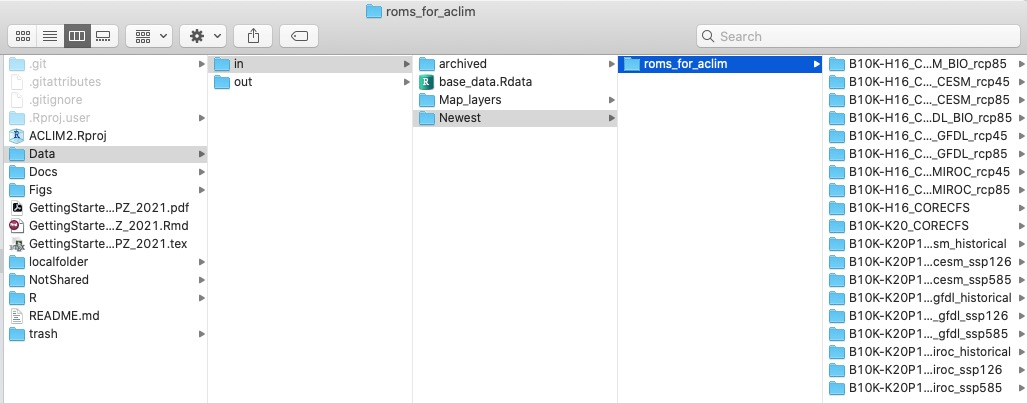
\includegraphics[width=1\textwidth,height=\textheight]{Figs/data_dir.jpg}
\caption{Your local \texttt{ACLIM2/Data} directory should look something
like this when you are done downloading the data and unzipping it.}
\end{figure}

\begin{figure}
\centering
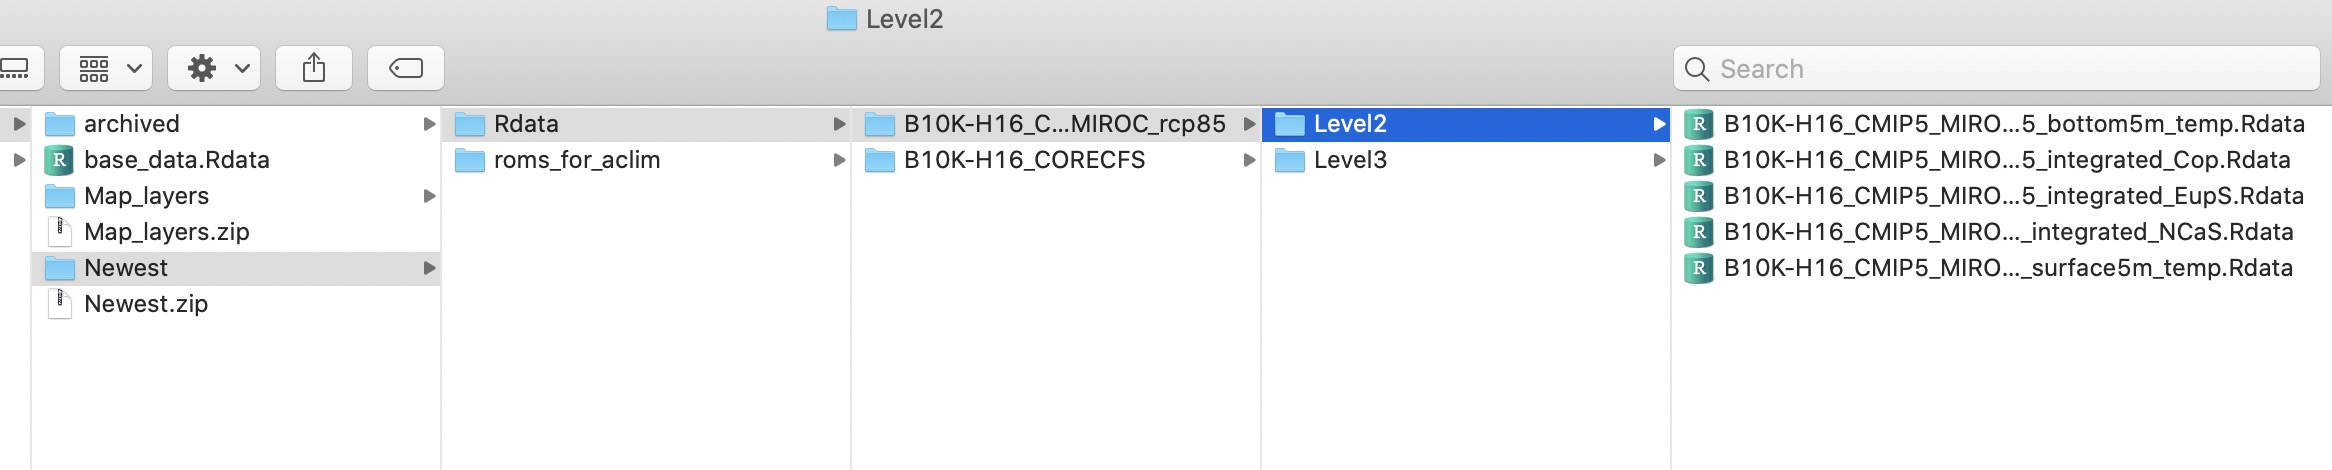
\includegraphics[width=1\textwidth,height=\textheight]{Figs/filestructure.jpg}
\caption{The final folder structure on your local drive in
\texttt{Data/in/Newest} should look something like this.}
\end{figure}

Now let's convert the CMIP6 Level3 .nc files to .Rdata files (as in
section 3.2.3)

\begin{Shaded}
\begin{Highlighting}[]
    \CommentTok{# preview the available CMIP6 data}
    \KeywordTok{dir}\NormalTok{(}\KeywordTok{file.path}\NormalTok{(local_fl,}\StringTok{"roms_for_aclim"}\NormalTok{))}
    
    \CommentTok{# variable list}
\NormalTok{    vl        <-}\StringTok{ }\KeywordTok{c}\NormalTok{(}
                  \StringTok{"temp_bottom5m"}\NormalTok{,}
                  \StringTok{"NCaS_integrated"}\NormalTok{, }\CommentTok{# Large Cop}
                  \StringTok{"Cop_integrated"}\NormalTok{,  }\CommentTok{# Small Cop}
                  \StringTok{"EupS_integrated"}\NormalTok{) }\CommentTok{# Euphausiids}

  \CommentTok{# define the simulation to download:}
\NormalTok{    cmip <-}\StringTok{ "CMIP6"}     \CommentTok{# Coupled Model Intercomparison Phase}
\NormalTok{    GCM  <-}\StringTok{ "MIROC"}     \CommentTok{# Global Circulation Model}
\NormalTok{    rcp  <-}\StringTok{ "ssp585"}     \CommentTok{# future carbon scenario}
\NormalTok{    mod  <-}\StringTok{ "B10K-K20P19"}  \CommentTok{# ROMSNPZ model}
\NormalTok{    hind <-}\StringTok{ "CORECFS"}      \CommentTok{# Hindcast}
    
    \CommentTok{# define the projection simulation:}
\NormalTok{    proj  <-}\StringTok{ }\KeywordTok{paste0}\NormalTok{(mod,}\StringTok{"_"}\NormalTok{,cmip,}\StringTok{"_"}\NormalTok{,GCM,}\StringTok{"_"}\NormalTok{,rcp)}
\NormalTok{    hind  <-}\StringTok{ }\KeywordTok{paste0}\NormalTok{(}\StringTok{"B10K-K20"}\NormalTok{,}\StringTok{"_"}\NormalTok{,hind)}
\NormalTok{    sl    <-}\StringTok{ }\KeywordTok{c}\NormalTok{(hind, proj)}
    
    \CommentTok{# opt 3:  convert subset of nc files to rdata files for analysis:}
    \KeywordTok{get_l3}\NormalTok{(}\DataTypeTok{web_nc =}\NormalTok{ F, }\DataTypeTok{download_nc =}\NormalTok{ F,}
          \DataTypeTok{local_path =} \KeywordTok{file.path}\NormalTok{(local_fl,}\StringTok{"roms_for_aclim"}\NormalTok{),}
          \DataTypeTok{varlist =}\NormalTok{ vl,}\DataTypeTok{sim_list =}\NormalTok{ sl)}
\end{Highlighting}
\end{Shaded}

\hypertarget{explore-indices-plot-the-data}{%
\section{4. Explore indices \& plot the
data}\label{explore-indices-plot-the-data}}

\hypertarget{a-quick-intro-to-level-2-and-3-data}{%
\subsection{4.1. A quick intro to Level 2 and 3
data}\label{a-quick-intro-to-level-2-and-3-data}}

KERIM's text and example here

\hypertarget{level-3-indices}{%
\subsection{4.2. Level 3 indices:}\label{level-3-indices}}

Level 3 indices can be used to generate seasonal, monthly, and annual
indices (like those reported in
\href{https://www.frontiersin.org/articles/10.3389/fmars.2020.00124/full}{Reum
et al.~2020)},
\href{http://dx.doi.org/10.1038/s41467-020-18300-3}{Holsman et
al.~2020)}. In the section below we explore these indices in more detail
using R, including using (2) above to generate weekly, monthly, and
seasonal indices (e.g.~Fall Zooplankton) for use in biological models.
In section 3 below we explore these indices in more detail using R,
including using (2) above to generate weekly, monthly, and seasonal
indices (e.g.~Fall Zooplankton) for use in biological models. The
following examples show how to analyze and plot the ACLIM indices from
the .Rdata files created in the previous step 3.

Please be sure to coordinate with ROMSNPZ modeling team members to
ensure data is applied appropriately. If you need access to the raw
ROMSNPZ files (netcdf, non-regridded large files located on MOX). Please
contact \href{albert.j.hermann@noaa.gov}{\textbf{Al Hermann}} or
\href{kelly.kearney@noaa.gov}{\textbf{Kelly Kearney}}. Please note that
while the CMIP5 set is now public (Hermann et al.~2019) \textbf{the
CMIP6 suite is under embargo for QAQC and should not be shared outside
of the ACLIM group}. See Section 1 above for more detail.

\hypertarget{explore-level-3-data-catalog}{%
\subsubsection{4.1.1 Explore Level 3 data
catalog}\label{explore-level-3-data-catalog}}

Once the base files and setup are loaded you can explore the index
types. Recall that in each scenario folder there are two indices saved
within the \texttt{Level3} subfolders:

\begin{enumerate}
\def\labelenumi{\arabic{enumi})}
\tightlist
\item
  \texttt{ACLIMsurveyrep\_B10K-x.nc} contains summer groundfish trawl
  ``survey replicated'' indices (using mean date and lat lon)
  \emph{(Note that the resampling stations need to be removed before
  creating bottom temperature maps)}\\
\item
  \texttt{ACLIMregion\_B10K-x.nc}: contains weekly ``strata'' values
  \emph{(Note that area weighting should be used to combine values
  across multiple strata)}
\end{enumerate}

First run the below set of code to set up the workspace:

\begin{Shaded}
\begin{Highlighting}[]
    \CommentTok{# --------------------------------------}
    \CommentTok{# SETUP WORKSPACE}
\NormalTok{    tmstp  <-}\StringTok{ }\KeywordTok{format}\NormalTok{(}\KeywordTok{Sys.time}\NormalTok{(), }\StringTok{"%Y_%m_%d"}\NormalTok{)}
\NormalTok{    main   <-}\StringTok{ }\KeywordTok{getwd}\NormalTok{()  }\CommentTok{#"~/GitHub_new/ACLIM2}
    \KeywordTok{source}\NormalTok{(}\StringTok{"R/make.R"}\NormalTok{)}
    \CommentTok{# --------------------------------------}
    
    \CommentTok{# list of the scenario x GCM downscaled ACLIM indices}
    \ControlFlowTok{for}\NormalTok{(k }\ControlFlowTok{in}\NormalTok{ aclim)}
     \KeywordTok{cat}\NormalTok{(}\KeywordTok{paste}\NormalTok{(k,}\StringTok{"}\CharTok{\textbackslash{}n}\StringTok{"}\NormalTok{))}
    
\NormalTok{    embargoed }\CommentTok{# not yet public or published}
\NormalTok{    public    }\CommentTok{# published runs (CMIP5)}
    
    \CommentTok{# get some info about a scenario:}
\NormalTok{    all_info1}
\NormalTok{    all_info2}
   
    \CommentTok{# variables in each of the two files:}
\NormalTok{    srvy_vars}
\NormalTok{    weekly_vars}
  
    \CommentTok{#summary tables for variables}
\NormalTok{    srvy_var_def}
\NormalTok{    weekly_var_def}
    
    \CommentTok{# explore stations in the survey replicated data:}
    \KeywordTok{head}\NormalTok{(station_info)}
\end{Highlighting}
\end{Shaded}

\hypertarget{level-3-spatial-indices-survey-replicated}{%
\subsubsection{4.1.2 Level 3: Spatial indices (survey
replicated)}\label{level-3-spatial-indices-survey-replicated}}

Let's start b exploring the survey replicated values for each variable.
Steps 2 and 3 generated the Rdata files that are stored in the
\texttt{ACLIMsurveyrep\_B10K-{[}version\_CMIPx\_GCM\_RCP{]}.Rdata} in
each corresponding simulation folder.

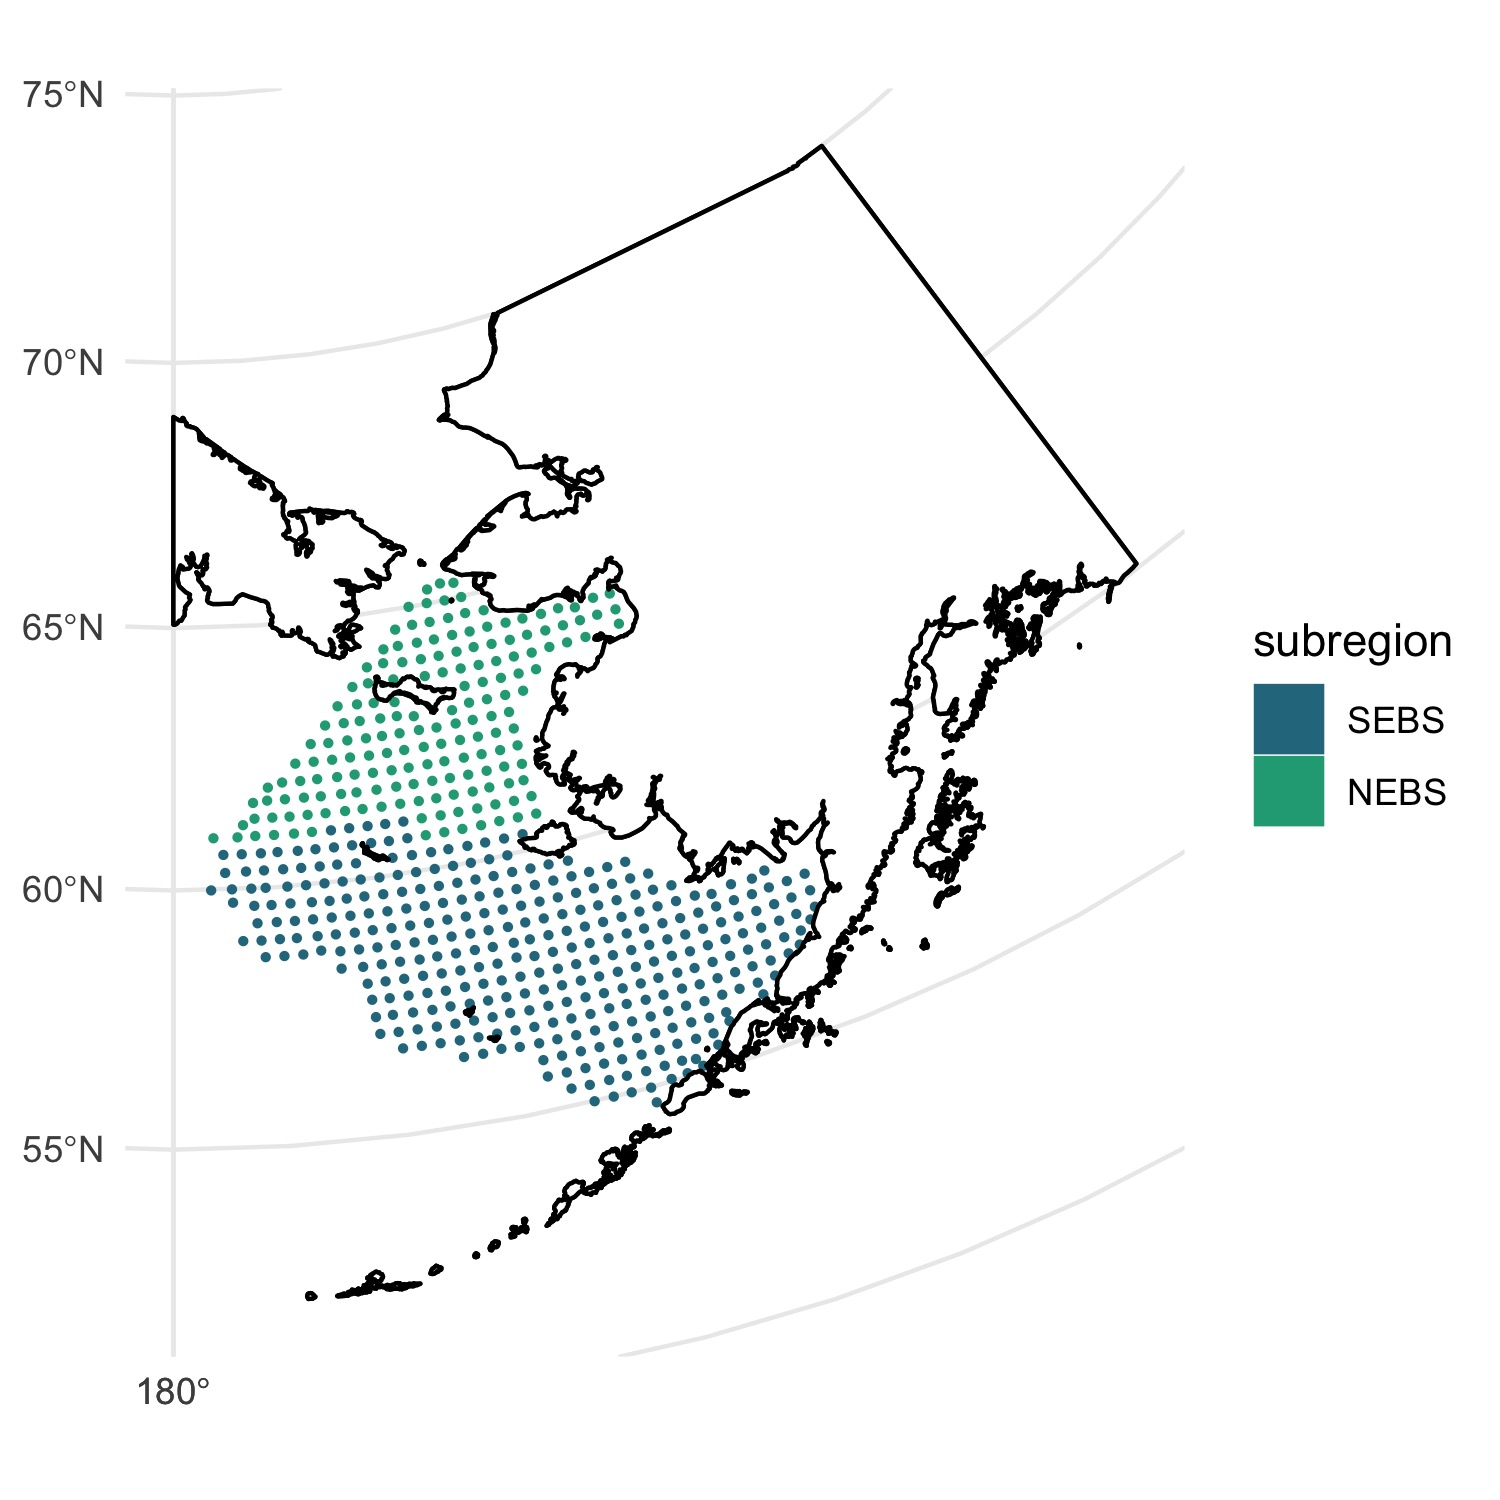
\includegraphics[width=0.5\textwidth,height=\textheight]{Figs/stations_NS.jpg}
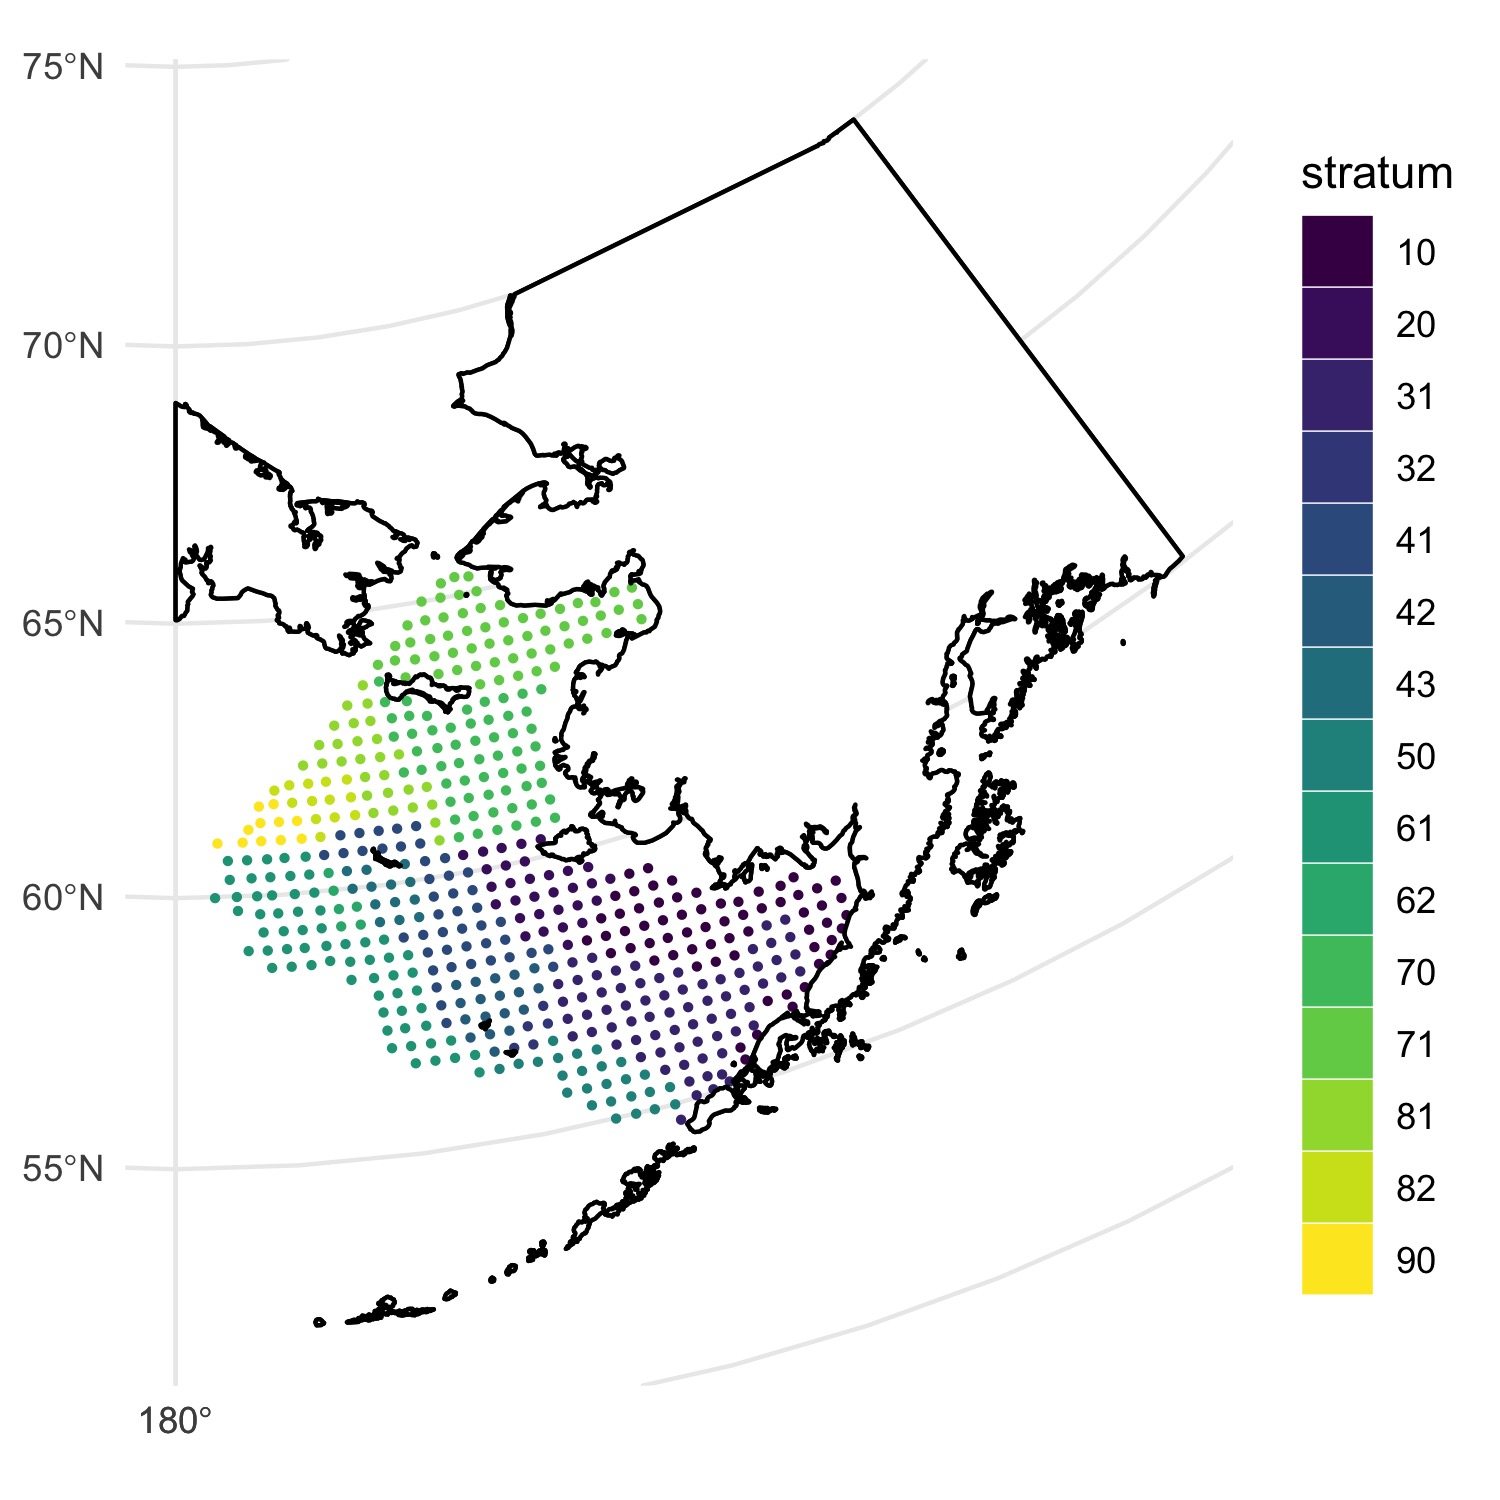
\includegraphics[width=0.5\textwidth,height=\textheight]{Figs/stations.jpg}

The code segment below will recreate the above figures.\emph{Note that
if this is the first time through it may take 3-5 mins to load the
spatial packages and download the files from the web (first time through
only).}

\begin{Shaded}
\begin{Highlighting}[]
   \CommentTok{# if load_gis is set to FALSE in R/setup.R (default) }
   \CommentTok{# we will need to load the gis layers and packages}
   \CommentTok{# if this is the first time through this would be a good time}
   \CommentTok{# to grab a coffee...}
   
   \KeywordTok{source}\NormalTok{(}\StringTok{"R/sub_scripts/load_maps.R"}\NormalTok{)}
  
   \CommentTok{# first convert the station_info object into a shapefile for mapping:}
\NormalTok{   station_sf         <-}\StringTok{ }\KeywordTok{convert2shp}\NormalTok{(station_info)}
\NormalTok{   station_sf}\OperatorTok{$}\NormalTok{stratum <-}\StringTok{ }\KeywordTok{factor}\NormalTok{(station_sf}\OperatorTok{$}\NormalTok{stratum)}
   
   \CommentTok{# plot the stations:}
\NormalTok{   p <-}\StringTok{ }\KeywordTok{plot_stations_basemap}\NormalTok{(}\DataTypeTok{sfIN =}\NormalTok{ station_sf,}
                              \DataTypeTok{fillIN =} \StringTok{"subregion"}\NormalTok{,}
                              \DataTypeTok{colorIN =} \StringTok{"subregion"}\NormalTok{) }\OperatorTok{+}\StringTok{ }
\StringTok{     }\KeywordTok{scale_color_viridis_d}\NormalTok{(}\DataTypeTok{begin =} \FloatTok{.2}\NormalTok{,}\DataTypeTok{end=}\NormalTok{.}\DecValTok{6}\NormalTok{) }\OperatorTok{+}
\StringTok{     }\KeywordTok{scale_fill_viridis_d}\NormalTok{(}\DataTypeTok{begin  =} \FloatTok{.2}\NormalTok{,}\DataTypeTok{end=}\NormalTok{.}\DecValTok{6}\NormalTok{)}
  
   \ControlFlowTok{if}\NormalTok{(update.figs)\{}
\NormalTok{     p}
     \KeywordTok{ggsave}\NormalTok{(}\DataTypeTok{file=}\KeywordTok{file.path}\NormalTok{(main,}\StringTok{"Figs/stations_NS.jpg"}\NormalTok{),}\DataTypeTok{width=}\DecValTok{5}\NormalTok{,}\DataTypeTok{height=}\DecValTok{5}\NormalTok{)}
\NormalTok{    \}}

\NormalTok{   p2 <-}\StringTok{ }\KeywordTok{plot_stations_basemap}\NormalTok{(}\DataTypeTok{sfIN =}\NormalTok{ station_sf,}\DataTypeTok{fillIN =} \StringTok{"stratum"}\NormalTok{,}\DataTypeTok{colorIN =} \StringTok{"stratum"}\NormalTok{) }\OperatorTok{+}\StringTok{ }
\StringTok{     }\KeywordTok{scale_color_viridis_d}\NormalTok{() }\OperatorTok{+}
\StringTok{     }\KeywordTok{scale_fill_viridis_d}\NormalTok{()}
   
   \ControlFlowTok{if}\NormalTok{(update.figs)\{}
\NormalTok{     p2}
   \KeywordTok{ggsave}\NormalTok{(}\DataTypeTok{file=}\KeywordTok{file.path}\NormalTok{(main,}\StringTok{"Figs/stations.jpg"}\NormalTok{),}\DataTypeTok{width=}\DecValTok{5}\NormalTok{,}\DataTypeTok{height=}\DecValTok{5}\NormalTok{)\}}
\end{Highlighting}
\end{Shaded}

\hypertarget{hindcasts}{%
\section{5. Hindcasts:}\label{hindcasts}}

There are two model versions of hindcasts available for comparison. The
Hermann et al.~2016 H16 10 depth layer model and the Kearney et al.~2020
30 depth layer model. Both are resolved spatially at a
\textasciitilde10km grid cell.

\hypertarget{level-3-hindcasts}{%
\subsection{5.1. Level 3 hindcasts}\label{level-3-hindcasts}}

Level 3 hindcast products inculde survey replicated station data and
strata averaged weekly values. The code below will explore these in more
detail.

\hypertarget{level-3-hindcasts-spatial-patterns}{%
\subsubsection{5.1.1. Level 3 hindcasts: spatial
patterns}\label{level-3-hindcasts-spatial-patterns}}

Now let's explore the survey replicated data in more detail and use to
plot bottom temperature.

\begin{Shaded}
\begin{Highlighting}[]
    \CommentTok{# run this line if load_gis is set to F in R/setup.R:}
    \KeywordTok{source}\NormalTok{(}\StringTok{"R/sub_scripts/load_maps.R"}\NormalTok{)  }

    \CommentTok{# preview the l3 data for the hindcast:}
\NormalTok{    tt <-}\StringTok{ }\NormalTok{all_info1}\OperatorTok\KeywordTok{filter}\NormalTok{(name }\OperatorTok{==}\StringTok{"B10K-K20_CORECFS"}\NormalTok{)}
\NormalTok{    tt <-}\StringTok{ }\KeywordTok{seq}\NormalTok{(}\KeywordTok{as.numeric}\NormalTok{(}\KeywordTok{substring}\NormalTok{(tt}\OperatorTok{$}\NormalTok{Start,}\DecValTok{1}\NormalTok{,}\DecValTok{4}\NormalTok{)),}\KeywordTok{as.numeric}\NormalTok{(}\KeywordTok{substring}\NormalTok{(tt}\OperatorTok{$}\NormalTok{End,}\DecValTok{1}\NormalTok{,}\DecValTok{4}\NormalTok{)),}\DecValTok{10}\NormalTok{)}
    
    \CommentTok{# now create plots of average BT during four time periods}
\NormalTok{    time_seg   <-}\StringTok{ }\KeywordTok{list}\NormalTok{( }\StringTok{'1970-1980'}\NormalTok{ =}\StringTok{ }\KeywordTok{c}\NormalTok{(}\DecValTok{1970}\OperatorTok{:}\DecValTok{1980}\NormalTok{),}
                        \StringTok{'1980-1990'}\NormalTok{ =}\StringTok{ }\KeywordTok{c}\NormalTok{(}\DecValTok{1980}\OperatorTok{:}\DecValTok{1990}\NormalTok{),}
                        \StringTok{'1990-2000'}\NormalTok{ =}\StringTok{ }\KeywordTok{c}\NormalTok{(}\DecValTok{1990}\OperatorTok{:}\DecValTok{2000}\NormalTok{),}
                        \StringTok{'2000-2010'}\NormalTok{ =}\StringTok{ }\KeywordTok{c}\NormalTok{(}\DecValTok{2000}\OperatorTok{:}\DecValTok{2010}\NormalTok{),}
                        \StringTok{'2010-2020'}\NormalTok{ =}\StringTok{ }\KeywordTok{c}\NormalTok{(}\DecValTok{2010}\OperatorTok{:}\DecValTok{2020}\NormalTok{))}
  
    \CommentTok{# lists the possible variables}
\NormalTok{    srvy_vars  }\CommentTok{# lists the possible variables}
    
    \CommentTok{# specify the variables to plot}
\NormalTok{    vl        <-}\StringTok{ }\KeywordTok{c}\NormalTok{(}
                  \StringTok{"temp_bottom5m"}\NormalTok{,}
                  \StringTok{"NCaS_integrated"}\NormalTok{, }\CommentTok{# Large Cop}
                  \StringTok{"Cop_integrated"}\NormalTok{,  }\CommentTok{# Small Cop}
                  \StringTok{"EupS_integrated"}\NormalTok{) }\CommentTok{# Euphausiids}
    
    \CommentTok{# assign the simulation to download}
    \CommentTok{# --> Tinker: try selecting a different set of models to compare}
\NormalTok{    sim        <-}\StringTok{"B10K-K20_CORECFS"} 
    
    \CommentTok{# open a "region" or strata specific nc file}
\NormalTok{    fl         <-}\StringTok{ }\KeywordTok{file.path}\NormalTok{(sim,}\KeywordTok{paste0}\NormalTok{(srvy_txt,sim,}\StringTok{".Rdata"}\NormalTok{))}
     
    \CommentTok{# create local rdata files (opt 1)}
    \ControlFlowTok{if}\NormalTok{(}\OperatorTok{!}\KeywordTok{file.exists}\NormalTok{(}\KeywordTok{file.path}\NormalTok{(Rdata_path,fl)))}
      \KeywordTok{get_l3}\NormalTok{(}\DataTypeTok{web_nc =} \OtherTok{TRUE}\NormalTok{, }\DataTypeTok{download_nc =}\NormalTok{ F,}
          \DataTypeTok{varlist =}\NormalTok{ vl,}\DataTypeTok{sim_list =}\NormalTok{sim )}
    
    \CommentTok{# load object 'ACLIMsurveyrep'}
    \KeywordTok{load}\NormalTok{(}\KeywordTok{file.path}\NormalTok{(main,Rdata_path,fl))   }
    
    
    \CommentTok{# Collate mean values across timeperiods and simulations}
    \CommentTok{# -------------------------------------------------------}
\NormalTok{    ms <-}\StringTok{ }\KeywordTok{c}\NormalTok{(}\StringTok{"B10K-H16_CORECFS"}\NormalTok{,}\StringTok{"B10K-K20_CORECFS"}\NormalTok{ )}
   
    \CommentTok{# Loop over model set}
    \ControlFlowTok{for}\NormalTok{(sim }\ControlFlowTok{in}\NormalTok{ ms)\{}
\NormalTok{     fl         <-}\StringTok{ }\KeywordTok{file.path}\NormalTok{(sim,}\KeywordTok{paste0}\NormalTok{(srvy_txt,sim,}\StringTok{".Rdata"}\NormalTok{))}
     
    \ControlFlowTok{if}\NormalTok{(}\OperatorTok{!}\KeywordTok{file.exists}\NormalTok{( }\KeywordTok{file.path}\NormalTok{(Rdata_path,fl)) )}
      \KeywordTok{get_l3}\NormalTok{(}\DataTypeTok{web_nc =} \OtherTok{TRUE}\NormalTok{, }\DataTypeTok{download_nc =}\NormalTok{ F,}
          \DataTypeTok{varlist =}\NormalTok{ vl,}\DataTypeTok{sim_list =}\NormalTok{sim )}
\NormalTok{    \}}
      
    \CommentTok{# get the mean values for the time blocks from the rdata versions}
    \CommentTok{# will throw "implicit NA" errors that can be ignored}
\NormalTok{    mn_var_all <-}\StringTok{ }\KeywordTok{get_mn_rd}\NormalTok{(}\DataTypeTok{modset =}\NormalTok{ ms,}
                            \DataTypeTok{names  =} \KeywordTok{c}\NormalTok{(}\StringTok{"H16"}\NormalTok{,}\StringTok{"K20"}\NormalTok{) ,}
                            \DataTypeTok{varUSE =} \StringTok{"temp_bottom5m"}\NormalTok{)}
    \CommentTok{# --> Tinker:           varUSE = "EupS_integrated") }
    
    \CommentTok{# convert results to a shapefile}
\NormalTok{    mn_var_sf  <-}\StringTok{ }\KeywordTok{convert2shp}\NormalTok{(mn_var_all}\OperatorTok\KeywordTok{filter}\NormalTok{(}\OperatorTok{!}\KeywordTok{is.na}\NormalTok{(mnval)))}
\NormalTok{    lab_t      <-}\StringTok{ "Bering10K CORECFS hindcast"}
    
\NormalTok{    p_hind_}\DecValTok{3}\NormalTok{         <-}\StringTok{ }\KeywordTok{plot_stations_basemap}\NormalTok{(}\DataTypeTok{sfIN =}\NormalTok{ mn_var_sf,}
                                \DataTypeTok{fillIN =} \StringTok{"mnval"}\NormalTok{,}
                                \DataTypeTok{colorIN =} \StringTok{"mnval"}\NormalTok{,}
                                \DataTypeTok{sizeIN=}\NormalTok{.}\DecValTok{3}\NormalTok{) }\OperatorTok{+}
\StringTok{      }\KeywordTok{facet_grid}\NormalTok{(simulation}\OperatorTok{~}\NormalTok{time_period)}\OperatorTok{+}
\StringTok{      }\KeywordTok{scale_color_viridis_c}\NormalTok{()}\OperatorTok{+}
\StringTok{      }\KeywordTok{scale_fill_viridis_c}\NormalTok{()}\OperatorTok{+}
\StringTok{      }\KeywordTok{guides}\NormalTok{(}
        \DataTypeTok{color =}  \KeywordTok{guide_legend}\NormalTok{(}\DataTypeTok{title=}\StringTok{"Bottom T (degC)"}\NormalTok{),}
        \DataTypeTok{fill  =}  \KeywordTok{guide_legend}\NormalTok{(}\DataTypeTok{title=}\StringTok{"Bottom T (degC)"}\NormalTok{)) }\OperatorTok{+}
\StringTok{      }\KeywordTok{ggtitle}\NormalTok{(lab_t)}
   
    \CommentTok{# This is slow but it works (repeat dev.new() twice if in Rstudio)...}
    \KeywordTok{dev.new}\NormalTok{()}
\NormalTok{    p_hind_}\DecValTok{3}
    
    \ControlFlowTok{if}\NormalTok{(update.figs)  }
      \KeywordTok{ggsave}\NormalTok{(}\DataTypeTok{file=}\KeywordTok{file.path}\NormalTok{(main,}\StringTok{"Figs/mn_hindcast_BT.jpg"}\NormalTok{),}\DataTypeTok{width=}\DecValTok{8}\NormalTok{,}\DataTypeTok{height=}\DecValTok{6}\NormalTok{)}
\end{Highlighting}
\end{Shaded}

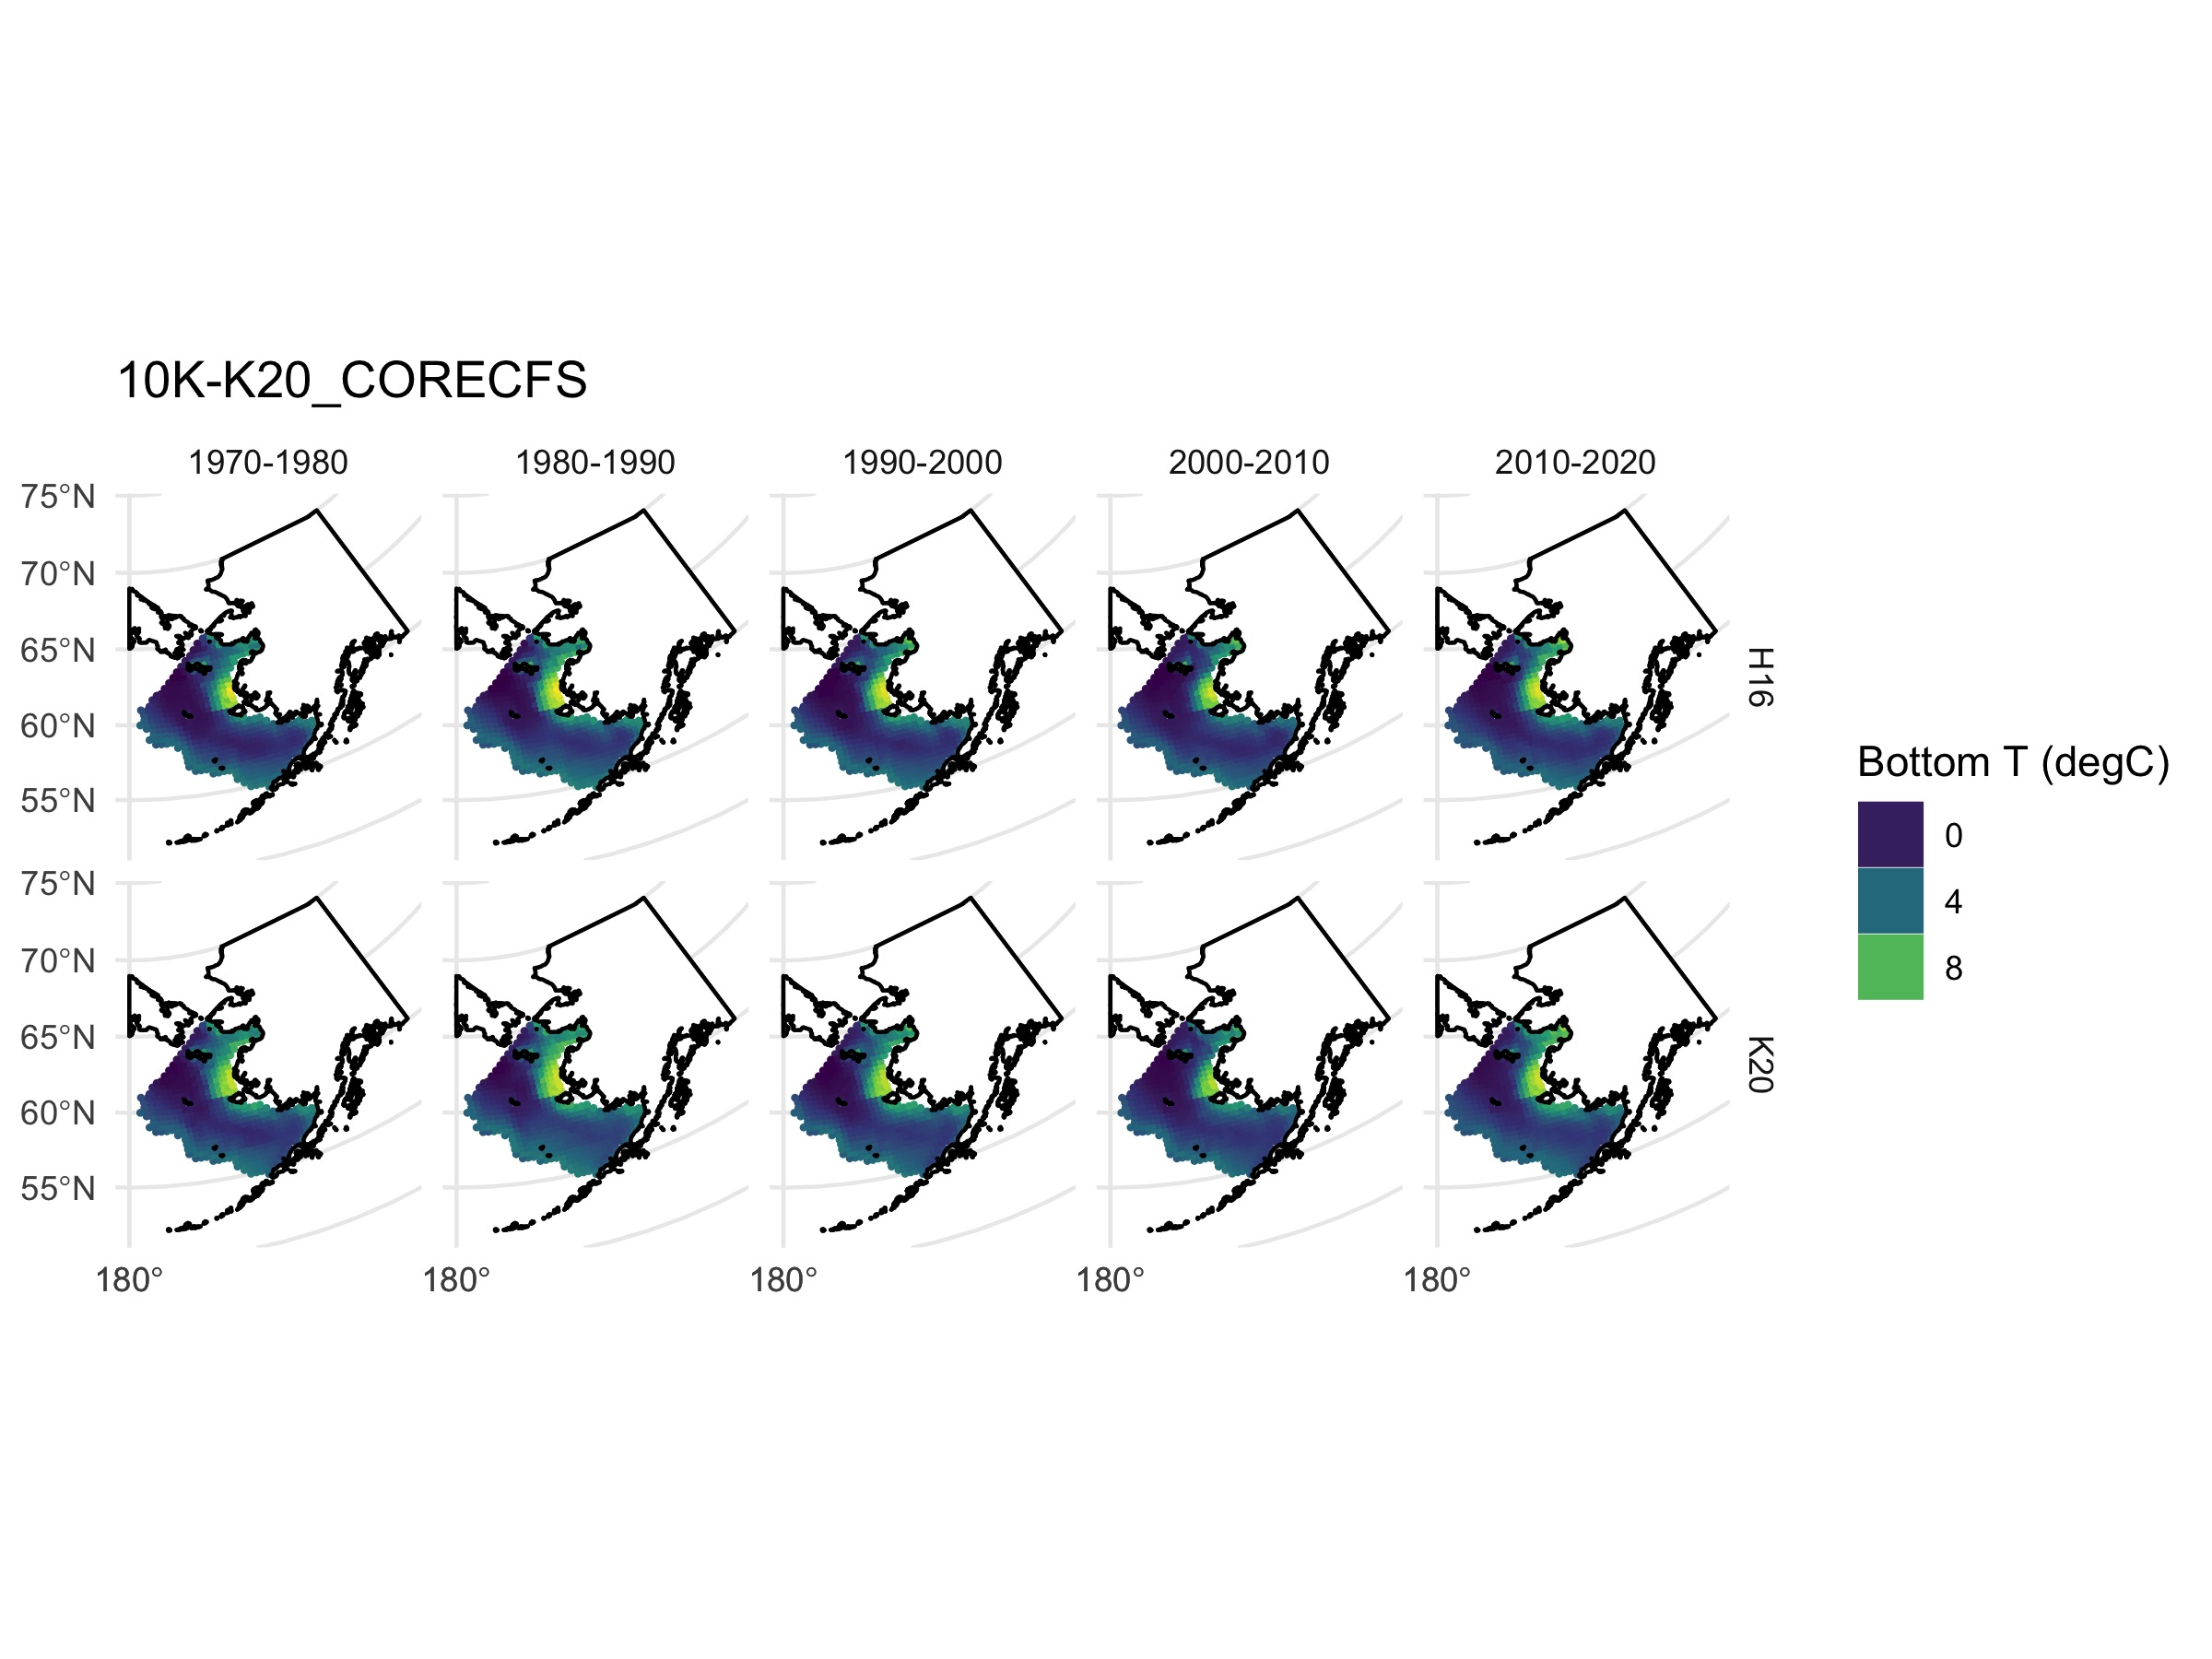
\includegraphics[width=1\textwidth,height=\textheight]{Figs/mn_hindcast_BT.jpg}
Now let's look at the Marine Heatwave conditions in 2018 and compare
that to the average conditions prior to 2010:

\begin{Shaded}
\begin{Highlighting}[]
    \CommentTok{# now create plots of average BT during four time periods}
\NormalTok{    time_seg   <-}\StringTok{ }\KeywordTok{list}\NormalTok{( }\StringTok{'1970-2010'}\NormalTok{ =}\StringTok{ }\KeywordTok{c}\NormalTok{(}\DecValTok{1970}\OperatorTok{:}\DecValTok{2010}\NormalTok{),}
                        \StringTok{'2018-2018'}\NormalTok{ =}\StringTok{ }\KeywordTok{c}\NormalTok{(}\DecValTok{2018}\OperatorTok{:}\DecValTok{2018}\NormalTok{))}
  
    \CommentTok{# assign the simulation to download}
\NormalTok{    sim        <-}\StringTok{ "B10K-K20_CORECFS"} 
    
    \CommentTok{# open a "region" or strata specific nc file}
\NormalTok{    fl         <-}\StringTok{ }\KeywordTok{file.path}\NormalTok{(sim,}\KeywordTok{paste0}\NormalTok{(srvy_txt,sim,}\StringTok{".Rdata"}\NormalTok{))}
     
    \CommentTok{# load object 'ACLIMsurveyrep'}
    \KeywordTok{load}\NormalTok{(}\KeywordTok{file.path}\NormalTok{(main,Rdata_path,fl))   }
      
    \CommentTok{# get the mean values for the time blocks from the rdata versions}
\NormalTok{    mn_var_all <-}\StringTok{ }\KeywordTok{get_mn_rd}\NormalTok{(}\DataTypeTok{modset =} \StringTok{"B10K-K20_CORECFS"}\NormalTok{,}
                            \DataTypeTok{varUSE =} \StringTok{"temp_bottom5m"}\NormalTok{)}
    
    \CommentTok{# convert results to a shapefile}
\NormalTok{    mn_var_sf  <-}\StringTok{ }\KeywordTok{convert2shp}\NormalTok{(mn_var_all}\OperatorTok\KeywordTok{filter}\NormalTok{(}\OperatorTok{!}\KeywordTok{is.na}\NormalTok{(mnval)))}
\NormalTok{    lab_t      <-}\StringTok{ "Bering10K CORECFS hindcast"}
    
\NormalTok{    p_mhw      <-}\StringTok{ }\KeywordTok{plot_stations_basemap}\NormalTok{(}\DataTypeTok{sfIN =}\NormalTok{ mn_var_sf,}
                                \DataTypeTok{fillIN =} \StringTok{"mnval"}\NormalTok{,}
                                \DataTypeTok{colorIN =} \StringTok{"mnval"}\NormalTok{,}
                                \DataTypeTok{sizeIN=}\NormalTok{.}\DecValTok{3}\NormalTok{) }\OperatorTok{+}
\StringTok{      }\KeywordTok{facet_grid}\NormalTok{(simulation}\OperatorTok{~}\NormalTok{time_period)}\OperatorTok{+}
\StringTok{      }\KeywordTok{scale_color_viridis_c}\NormalTok{()}\OperatorTok{+}
\StringTok{      }\KeywordTok{scale_fill_viridis_c}\NormalTok{()}\OperatorTok{+}
\StringTok{      }\KeywordTok{guides}\NormalTok{(}
        \DataTypeTok{color =}  \KeywordTok{guide_legend}\NormalTok{(}\DataTypeTok{title=}\StringTok{"Bottom T (degC)"}\NormalTok{),}
        \DataTypeTok{fill  =}  \KeywordTok{guide_legend}\NormalTok{(}\DataTypeTok{title=}\StringTok{"Bottom T (degC)"}\NormalTok{)) }\OperatorTok{+}
\StringTok{      }\KeywordTok{ggtitle}\NormalTok{(lab_t)}
   
    \CommentTok{# This is slow but it works (repeat dev.new() twice if in Rstudio)...}
    \KeywordTok{dev.new}\NormalTok{(}\DataTypeTok{width=}\DecValTok{4}\NormalTok{,}\DataTypeTok{height=}\DecValTok{3}\NormalTok{)}
\NormalTok{    p_mhw}
    
    \ControlFlowTok{if}\NormalTok{(update.figs)  }
      \KeywordTok{ggsave}\NormalTok{(}\DataTypeTok{file=}\KeywordTok{file.path}\NormalTok{(main,}\StringTok{"Figs/mn_hindcast_mhw.jpg"}\NormalTok{),}\DataTypeTok{width=}\DecValTok{4}\NormalTok{,}\DataTypeTok{height=}\DecValTok{3}\NormalTok{)}
\end{Highlighting}
\end{Shaded}

\begin{figure}
\centering
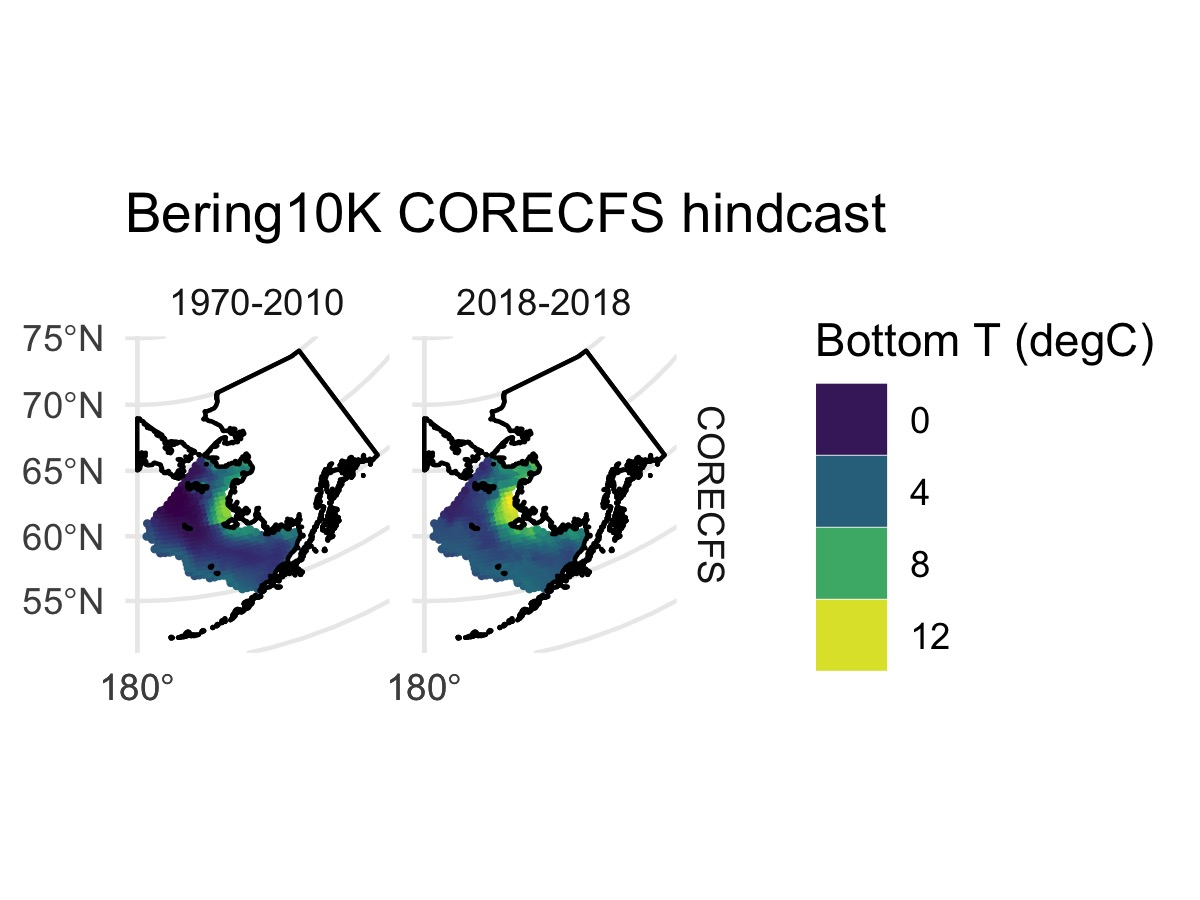
\includegraphics[width=0.75\textwidth,height=\textheight]{Figs/mn_hindcast_mhw.jpg}
\caption{Decadal averages of bottom temperature from the two hindcast
models.}
\end{figure}

\hypertarget{level-3-hindcasts-weekly-strata-averages}{%
\subsubsection{5.1.2. Level 3 hindcasts: Weekly strata
averages}\label{level-3-hindcasts-weekly-strata-averages}}

The next set of indices to will explore are the weekly strata-specific
values for each variable.These are stored in the
\texttt{ACLIMregion\_B10K-{[}version\_CMIPx\_GCM\_RCP{]}.nc} in each
scenario folder.

\begin{Shaded}
\begin{Highlighting}[]
    \CommentTok{# View an individual variable (e.g., Bottom Temp)}
    \CommentTok{# -------------------------------------------------------}
\NormalTok{    weekly_vars}

    \CommentTok{# assign the simulation to download}
\NormalTok{    sim        <-}\StringTok{ "B10K-K20_CORECFS"} 
    
    \CommentTok{# define a "region" or strata specific nc file}
\NormalTok{    fl         <-}\StringTok{ }\KeywordTok{file.path}\NormalTok{(sim,}\KeywordTok{paste0}\NormalTok{(reg_txt,sim,}\StringTok{".Rdata"}\NormalTok{))}
    

\NormalTok{    vl        <-}\StringTok{ }\KeywordTok{c}\NormalTok{(}
                  \StringTok{"temp_bottom5m"}\NormalTok{,}
                  \StringTok{"NCaS_integrated"}\NormalTok{, }\CommentTok{# Large Cop}
                  \StringTok{"Cop_integrated"}\NormalTok{,  }\CommentTok{# Small Cop}
                  \StringTok{"EupS_integrated"}\NormalTok{) }\CommentTok{# Euphausiids}
    
    \CommentTok{# create local rdata files (opt 1)}
    \ControlFlowTok{if}\NormalTok{(}\OperatorTok{!}\KeywordTok{file.exists}\NormalTok{(}\KeywordTok{file.path}\NormalTok{(Rdata_path,fl)))}
      \KeywordTok{get_l3}\NormalTok{(}\DataTypeTok{web_nc =} \OtherTok{TRUE}\NormalTok{, }\DataTypeTok{download_nc =}\NormalTok{ F,}
          \DataTypeTok{varlist =}\NormalTok{ vl,}\DataTypeTok{sim_list =}\NormalTok{ sim)}
    
 
    \CommentTok{# load object 'ACLIMregion' for bottom temperature}
    \KeywordTok{load}\NormalTok{(}\KeywordTok{file.path}\NormalTok{(main,Rdata_path,fl))  }
\NormalTok{    tmp_var    <-}\StringTok{ }\NormalTok{ACLIMregion}\OperatorTok\KeywordTok{filter}\NormalTok{(var }\OperatorTok{==}\StringTok{ "temp_bottom5m"}\NormalTok{)}
    
   \CommentTok{# now plot the data:}
\NormalTok{   p4_hind <-}\StringTok{ }\KeywordTok{ggplot}\NormalTok{(}\DataTypeTok{data =}\NormalTok{ tmp_var) }\OperatorTok{+}\StringTok{ }
\StringTok{     }\KeywordTok{geom_line}\NormalTok{(}\KeywordTok{aes}\NormalTok{(}\DataTypeTok{x=}\NormalTok{time,}\DataTypeTok{y=}\NormalTok{val,}\DataTypeTok{color=}\NormalTok{ strata),}\DataTypeTok{alpha=}\NormalTok{.}\DecValTok{8}\NormalTok{)}\OperatorTok{+}
\StringTok{     }\KeywordTok{facet_grid}\NormalTok{(basin}\OperatorTok{~}\NormalTok{.)}\OperatorTok{+}
\StringTok{     }\KeywordTok{ylab}\NormalTok{(tmp_var}\OperatorTok{$}\NormalTok{units[}\DecValTok{1}\NormalTok{])}\OperatorTok{+}
\StringTok{     }\KeywordTok{ggtitle}\NormalTok{( }\KeywordTok{paste}\NormalTok{(sim,tmp_var}\OperatorTok{$}\NormalTok{var[}\DecValTok{1}\NormalTok{]))}\OperatorTok{+}
\StringTok{     }\KeywordTok{theme_minimal}\NormalTok{()}
\NormalTok{   p4_hind}
   
    \ControlFlowTok{if}\NormalTok{(update.figs)  }
      \KeywordTok{ggsave}\NormalTok{(}\DataTypeTok{file=}\KeywordTok{file.path}\NormalTok{(main,}\StringTok{"Figs/hind_weekly_bystrata.jpg"}\NormalTok{),}\DataTypeTok{width=}\DecValTok{8}\NormalTok{,}\DataTypeTok{height=}\DecValTok{5}\NormalTok{)}

   
   \CommentTok{# To get the average value for a set of strata, weight the val by the area:}
\NormalTok{   mn_NEBS <-}\StringTok{ }\KeywordTok{getAVGnSUM}\NormalTok{(}\DataTypeTok{strataIN =}\NormalTok{ NEBS_strata, }\DataTypeTok{dataIN =}\NormalTok{ tmp_var)}
\NormalTok{   mn_NEBS}\OperatorTok{$}\NormalTok{basin =}\StringTok{ "NEBS"}
\NormalTok{   mn_SEBS <-}\KeywordTok{getAVGnSUM}\NormalTok{(}\DataTypeTok{strataIN =}\NormalTok{ SEBS_strata, }\DataTypeTok{dataIN =}\NormalTok{ tmp_var)}
\NormalTok{   mn_SEBS}\OperatorTok{$}\NormalTok{basin =}\StringTok{ "SEBS"}
   
\NormalTok{   p5_hind <-}\StringTok{ }\KeywordTok{ggplot}\NormalTok{(}\DataTypeTok{data =} \KeywordTok{rbind}\NormalTok{(mn_NEBS,mn_SEBS)) }\OperatorTok{+}\StringTok{ }
\StringTok{      }\KeywordTok{geom_line}\NormalTok{(}\KeywordTok{aes}\NormalTok{(}\DataTypeTok{x=}\NormalTok{time,}\DataTypeTok{y=}\NormalTok{mn_val,}\DataTypeTok{color=}\NormalTok{basin),}\DataTypeTok{alpha=}\NormalTok{.}\DecValTok{8}\NormalTok{)}\OperatorTok{+}
\StringTok{      }\KeywordTok{geom_smooth}\NormalTok{(}\KeywordTok{aes}\NormalTok{(}\DataTypeTok{x=}\NormalTok{time,}\DataTypeTok{y=}\NormalTok{mn_val,}\DataTypeTok{color=}\NormalTok{basin),}
                  \DataTypeTok{formula =}\NormalTok{ y }\OperatorTok{~}\StringTok{ }\NormalTok{x, }\DataTypeTok{se =}\NormalTok{ T)}\OperatorTok{+}
\StringTok{      }\KeywordTok{facet_grid}\NormalTok{(basin}\OperatorTok{~}\NormalTok{.)}\OperatorTok{+}
\StringTok{      }\KeywordTok{scale_color_viridis_d}\NormalTok{(}\DataTypeTok{begin=}\NormalTok{.}\DecValTok{4}\NormalTok{,}\DataTypeTok{end=}\NormalTok{.}\DecValTok{8}\NormalTok{)}\OperatorTok{+}
\StringTok{      }\KeywordTok{ylab}\NormalTok{(tmp_var}\OperatorTok{$}\NormalTok{units[}\DecValTok{1}\NormalTok{])}\OperatorTok{+}
\StringTok{      }\KeywordTok{ggtitle}\NormalTok{( }\KeywordTok{paste}\NormalTok{(sim,mn_NEBS}\OperatorTok{$}\NormalTok{var[}\DecValTok{1}\NormalTok{]))}\OperatorTok{+}
\StringTok{     }
\StringTok{      }\KeywordTok{theme_minimal}\NormalTok{()}
\NormalTok{  p5_hind}
  \ControlFlowTok{if}\NormalTok{(update.figs)  }
    \KeywordTok{ggsave}\NormalTok{(}\DataTypeTok{file=}\KeywordTok{file.path}\NormalTok{(main,}\StringTok{"Figs/hind_weekly_byreg.jpg"}\NormalTok{),}\DataTypeTok{width=}\DecValTok{8}\NormalTok{,}\DataTypeTok{height=}\DecValTok{5}\NormalTok{)}
\end{Highlighting}
\end{Shaded}

\begin{figure}
\centering
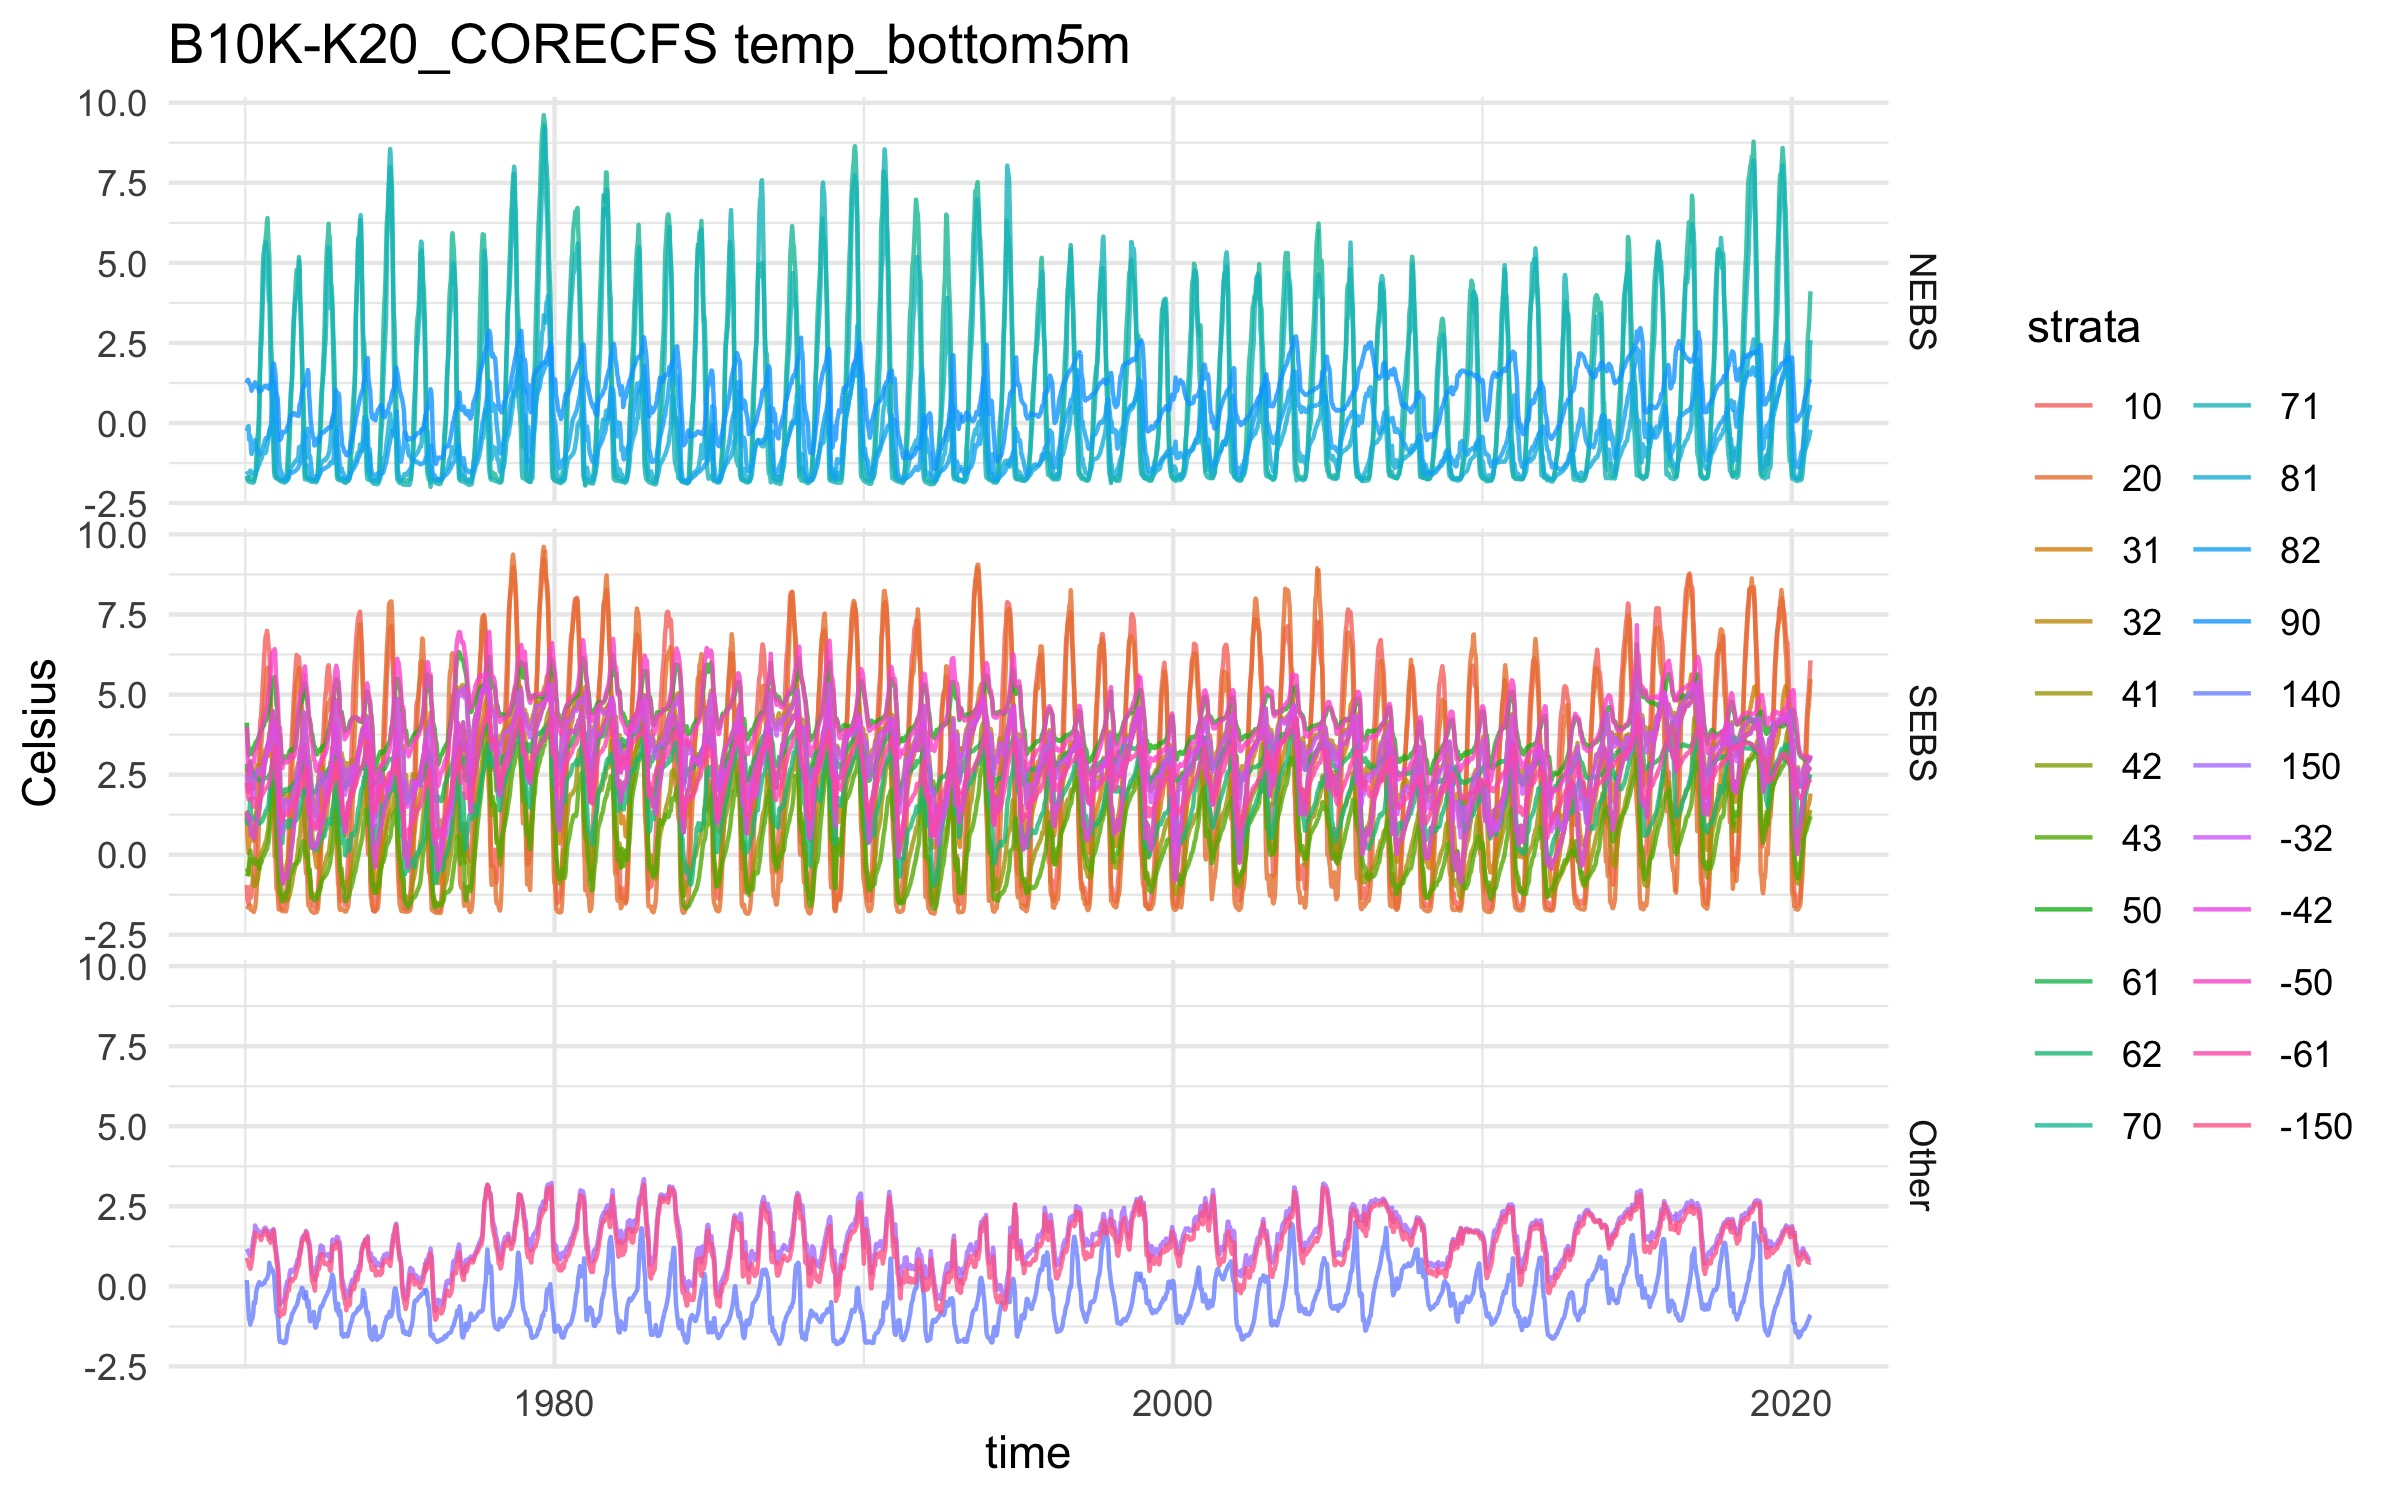
\includegraphics[width=0.65\textwidth,height=\textheight]{Figs/hind_weekly_bystrata.jpg}
\caption{Weekly indcices by sub-region}
\end{figure}

\begin{figure}
\centering
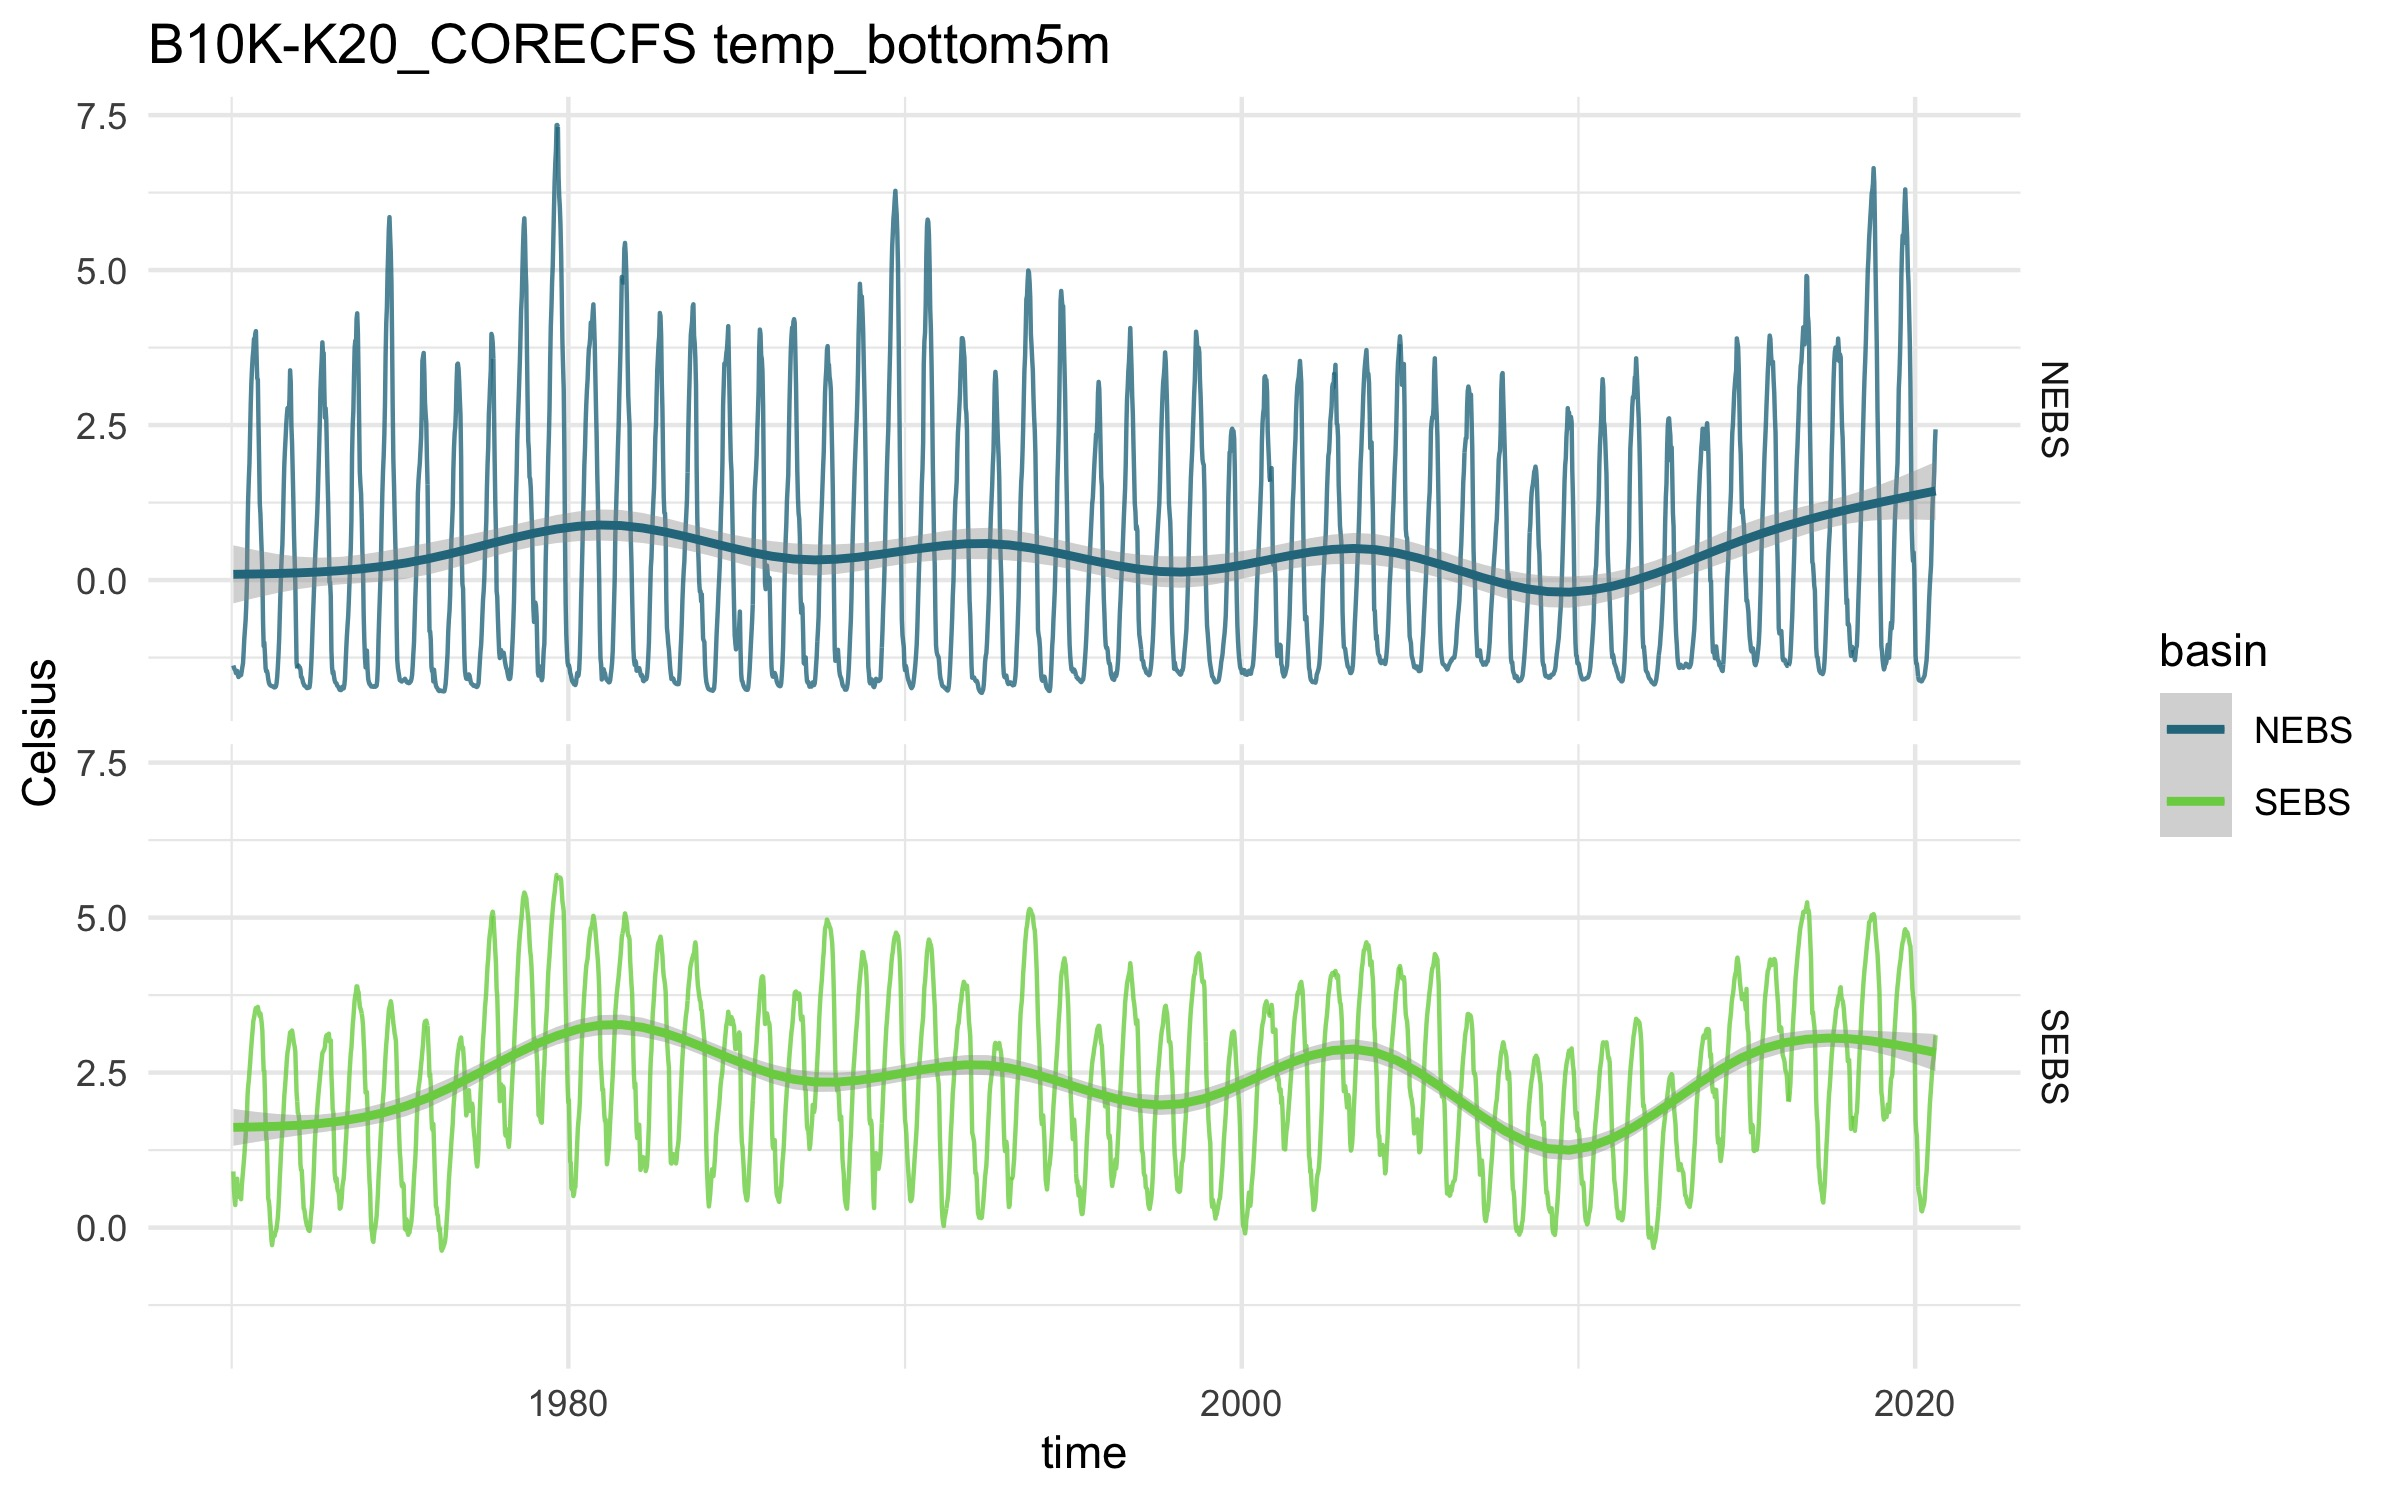
\includegraphics[width=0.65\textwidth,height=\textheight]{Figs/hind_weekly_byreg.jpg}
\caption{Weekly indcices by sub-region}
\end{figure}

\hypertarget{level-3-hindcasts-seasonal-averages}{%
\subsubsection{5.1.3. Level 3 hindcasts: Seasonal
averages}\label{level-3-hindcasts-seasonal-averages}}

Now using a similar approach get the monthly mean values for a variable:

\begin{Shaded}
\begin{Highlighting}[]
    \CommentTok{# assign the simulation to download}
\NormalTok{      sim        <-}\StringTok{ "B10K-K20_CORECFS"} 
   

    \CommentTok{# Set up seasons (this follows Holsman et al. 2020)}
\NormalTok{      seasons <-}\StringTok{ }\KeywordTok{data.frame}\NormalTok{(}\DataTypeTok{mo =} \DecValTok{1}\OperatorTok{:}\DecValTok{12}\NormalTok{, }
                   \DataTypeTok{season =}\KeywordTok{factor}\NormalTok{(}\StringTok{""}\NormalTok{,}
                     \DataTypeTok{levels=}\KeywordTok{c}\NormalTok{(}\StringTok{"Winter"}\NormalTok{,}\StringTok{"Spring"}\NormalTok{,}\StringTok{"Summer"}\NormalTok{,}\StringTok{"Fall"}\NormalTok{)))}
\NormalTok{      seasons}\OperatorTok{$}\NormalTok{season[}\DecValTok{1}\OperatorTok{:}\DecValTok{3}\NormalTok{]   <-}\StringTok{ "Winter"}
\NormalTok{      seasons}\OperatorTok{$}\NormalTok{season[}\DecValTok{4}\OperatorTok{:}\DecValTok{6}\NormalTok{]   <-}\StringTok{ "Spring"}
\NormalTok{      seasons}\OperatorTok{$}\NormalTok{season[}\DecValTok{7}\OperatorTok{:}\DecValTok{9}\NormalTok{]   <-}\StringTok{ "Summer"}
\NormalTok{      seasons}\OperatorTok{$}\NormalTok{season[}\DecValTok{10}\OperatorTok{:}\DecValTok{12}\NormalTok{] <-}\StringTok{ "Fall"}
    
       
\NormalTok{    vl <-}\StringTok{ }\KeywordTok{c}\NormalTok{(}
                  \StringTok{"temp_bottom5m"}\NormalTok{,}
                  \StringTok{"NCaS_integrated"}\NormalTok{, }\CommentTok{# Large Cop}
                  \StringTok{"Cop_integrated"}\NormalTok{,  }\CommentTok{# Small Cop}
                  \StringTok{"EupS_integrated"}\NormalTok{) }\CommentTok{# Euphausiids}
    
    \CommentTok{# create local rdata files (opt 1)}
    \ControlFlowTok{if}\NormalTok{(}\OperatorTok{!}\KeywordTok{file.exists}\NormalTok{(}\KeywordTok{file.path}\NormalTok{(Rdata_path,fl)))}
      \KeywordTok{get_l3}\NormalTok{(}\DataTypeTok{web_nc =} \OtherTok{TRUE}\NormalTok{, }\DataTypeTok{download_nc =}\NormalTok{ F,}
          \DataTypeTok{varlist =}\NormalTok{ vl,}\DataTypeTok{sim_list =}\NormalTok{ sim)}
    
    \CommentTok{# open a "region" or strata specific  file}
\NormalTok{    fl      <-}\StringTok{ }\KeywordTok{file.path}\NormalTok{(sim,}\KeywordTok{paste0}\NormalTok{(reg_txt,sim,}\StringTok{".Rdata"}\NormalTok{))}
    \KeywordTok{load}\NormalTok{(}\KeywordTok{file.path}\NormalTok{(main,Rdata_path,fl))}
    
    \CommentTok{# get large zooplankton as the sum of euph and NCaS}
\NormalTok{    tmp_var    <-}\StringTok{ }\NormalTok{ACLIMregion}\OperatorTok
\StringTok{      }\KeywordTok{filter}\NormalTok{(var}\OperatorTok\NormalTok{vl[}\KeywordTok{c}\NormalTok{(}\DecValTok{2}\NormalTok{,}\DecValTok{3}\NormalTok{)])}\OperatorTok
\StringTok{      }\KeywordTok{group_by}\NormalTok{(time,strata,strata_area_km2,basin)}\OperatorTok
\StringTok{      }\KeywordTok{group_by}\NormalTok{(time,}
\NormalTok{             strata,}
\NormalTok{             strata_area_km2,}
\NormalTok{             basin,}
\NormalTok{             units)}\OperatorTok
\StringTok{      }\KeywordTok{summarise}\NormalTok{(}\DataTypeTok{val =}\KeywordTok{sum}\NormalTok{(val))}\OperatorTok
\StringTok{      }\KeywordTok{mutate}\NormalTok{(}\DataTypeTok{var       =} \StringTok{"Zoop_integrated"}\NormalTok{,}
             \DataTypeTok{long_name =}\StringTok{"Total On-shelf }
\StringTok{             large zooplankton concentration, }
\StringTok{             integrated over depth (NCa, Eup)"}\NormalTok{)}
    
    \KeywordTok{rm}\NormalTok{(ACLIMregion)}
    \KeywordTok{head}\NormalTok{(tmp_var)}
    
    \CommentTok{# define some columns for year mo and julian day}
\NormalTok{    tmp_var}\OperatorTok{$}\NormalTok{yr     <-}\StringTok{ }\KeywordTok{strptime}\NormalTok{(}\KeywordTok{as.Date}\NormalTok{(tmp_var}\OperatorTok{$}\NormalTok{time),}
                               \DataTypeTok{format=}\StringTok{"%Y-%m-%d"}\NormalTok{)}\OperatorTok{$}\NormalTok{year }\OperatorTok{+}\StringTok{ }\DecValTok{1900}
\NormalTok{    tmp_var}\OperatorTok{$}\NormalTok{mo     <-}\StringTok{ }\KeywordTok{strptime}\NormalTok{(}\KeywordTok{as.Date}\NormalTok{(tmp_var}\OperatorTok{$}\NormalTok{time),}
                               \DataTypeTok{format=}\StringTok{"%Y-%m-%d"}\NormalTok{)}\OperatorTok{$}\NormalTok{mon  }\OperatorTok{+}\StringTok{ }\DecValTok{1}
\NormalTok{    tmp_var}\OperatorTok{$}\NormalTok{jday   <-}\StringTok{ }\KeywordTok{strptime}\NormalTok{(}\KeywordTok{as.Date}\NormalTok{(tmp_var}\OperatorTok{$}\NormalTok{time),}
                               \DataTypeTok{format=}\StringTok{"%Y-%m-%d"}\NormalTok{)}\OperatorTok{$}\NormalTok{yday }\OperatorTok{+}\StringTok{ }\DecValTok{1}
\NormalTok{    tmp_var}\OperatorTok{$}\NormalTok{season <-}\StringTok{ }\NormalTok{seasons[tmp_var}\OperatorTok{$}\NormalTok{mo,}\DecValTok{2}\NormalTok{]}
    
    \CommentTok{# To get the average value for a set of strata, weight the val by the area: (slow...)}
\NormalTok{    mn_NEBS_season <-}\StringTok{ }\KeywordTok{getAVGnSUM}\NormalTok{(}
      \DataTypeTok{strataIN =}\NormalTok{ NEBS_strata,}
      \DataTypeTok{dataIN =}\NormalTok{ tmp_var,}
      \DataTypeTok{tblock=}\KeywordTok{c}\NormalTok{(}\StringTok{"yr"}\NormalTok{,}\StringTok{"season"}\NormalTok{))}
\NormalTok{    mn_NEBS_season}\OperatorTok{$}\NormalTok{basin =}\StringTok{ "NEBS"}
    
\NormalTok{    mn_SEBS_season <-}\StringTok{ }\KeywordTok{getAVGnSUM}\NormalTok{(}
      \DataTypeTok{strataIN =}\NormalTok{ SEBS_strata, }
      \DataTypeTok{dataIN =}\NormalTok{ tmp_var,}
      \DataTypeTok{tblock=}\KeywordTok{c}\NormalTok{(}\StringTok{"yr"}\NormalTok{,}\StringTok{"season"}\NormalTok{))}
\NormalTok{    mn_SEBS_season}\OperatorTok{$}\NormalTok{basin =}\StringTok{ "SEBS"}
    
\NormalTok{   plot_data      <-}\StringTok{ }\KeywordTok{rbind}\NormalTok{(mn_NEBS_season,mn_SEBS_season)}
    
   \CommentTok{# plot Fall values:}
\NormalTok{   p6_hind <-}\StringTok{ }\KeywordTok{ggplot}\NormalTok{(}\DataTypeTok{data =}\NormalTok{ plot_data}\OperatorTok\KeywordTok{filter}\NormalTok{(season}\OperatorTok{==}\StringTok{"Fall"}\NormalTok{) ) }\OperatorTok{+}\StringTok{ }
\StringTok{      }\KeywordTok{geom_line}\NormalTok{(   }\KeywordTok{aes}\NormalTok{(}\DataTypeTok{x =}\NormalTok{ yr,}\DataTypeTok{y =}\NormalTok{ mn_val,}\DataTypeTok{color=}\NormalTok{basin),}\DataTypeTok{alpha=}\NormalTok{.}\DecValTok{8}\NormalTok{)}\OperatorTok{+}
\StringTok{      }\KeywordTok{geom_smooth}\NormalTok{( }\KeywordTok{aes}\NormalTok{(}\DataTypeTok{x =}\NormalTok{ yr,}\DataTypeTok{y =}\NormalTok{ mn_val,}\DataTypeTok{color=}\NormalTok{basin),}
                  \DataTypeTok{formula =}\NormalTok{ y }\OperatorTok{~}\StringTok{ }\NormalTok{x, }\DataTypeTok{se =}\NormalTok{ T)}\OperatorTok{+}
\StringTok{      }\KeywordTok{facet_grid}\NormalTok{(basin}\OperatorTok{~}\NormalTok{.)}\OperatorTok{+}
\StringTok{      }\KeywordTok{scale_color_viridis_d}\NormalTok{(}\DataTypeTok{begin=}\NormalTok{.}\DecValTok{4}\NormalTok{,}\DataTypeTok{end=}\NormalTok{.}\DecValTok{8}\NormalTok{)}\OperatorTok{+}
\StringTok{      }\KeywordTok{ylab}\NormalTok{(tmp_var}\OperatorTok{$}\NormalTok{units[}\DecValTok{1}\NormalTok{])}\OperatorTok{+}
\StringTok{      }\KeywordTok{ggtitle}\NormalTok{( }\KeywordTok{paste}\NormalTok{(sim,}\StringTok{"Fall"}\NormalTok{,mn_NEBS_season}\OperatorTok{$}\NormalTok{var[}\DecValTok{1}\NormalTok{]))}\OperatorTok{+}
\StringTok{      }\KeywordTok{theme_minimal}\NormalTok{()}
\NormalTok{  p6_hind}
  
  
  \ControlFlowTok{if}\NormalTok{(update.figs)  }
    \KeywordTok{ggsave}\NormalTok{(}\DataTypeTok{file=}\KeywordTok{file.path}\NormalTok{(main,}\StringTok{"Figs/Hind_Fall_large_Zoop.jpg"}\NormalTok{),}\DataTypeTok{width=}\DecValTok{8}\NormalTok{,}\DataTypeTok{height=}\DecValTok{5}\NormalTok{)}
\end{Highlighting}
\end{Shaded}

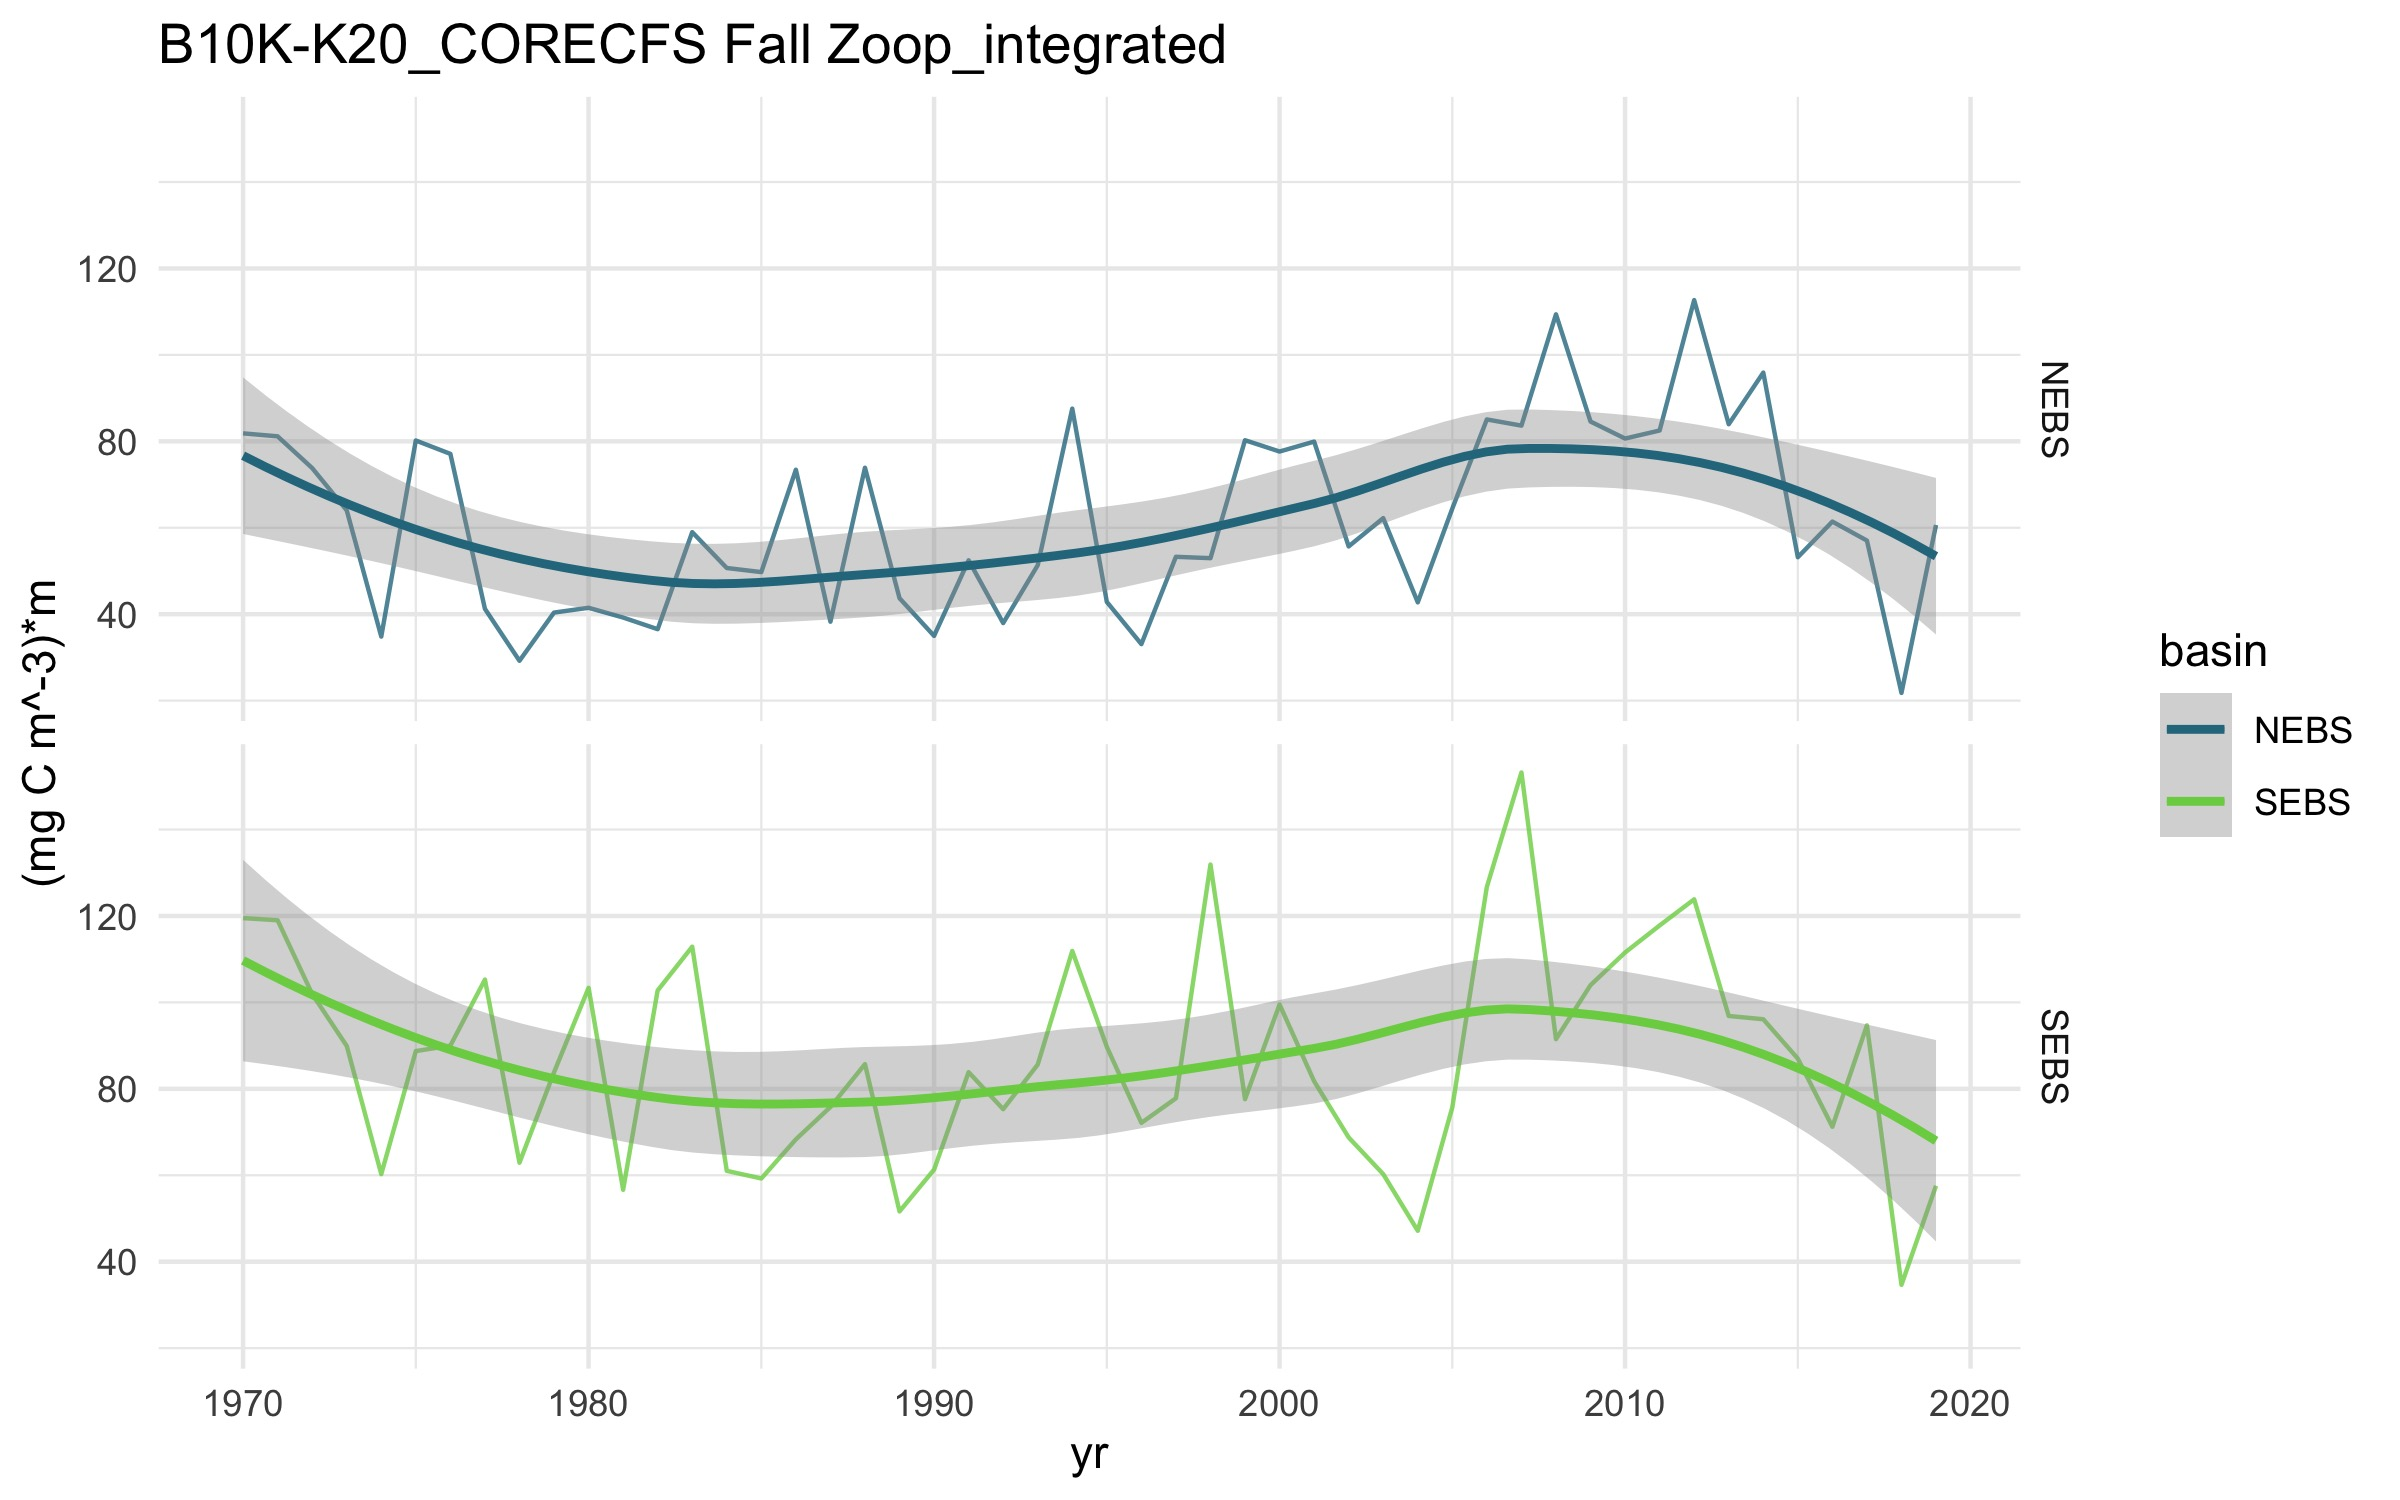
\includegraphics[width=0.65\textwidth,height=\textheight]{Figs/Hind_Fall_large_Zoop.jpg}
\#\#\# 5.1.4. Level 3 hindcasts: Monthly averages

Using the same approach we can get monthly averages for a given
variable:

\begin{Shaded}
\begin{Highlighting}[]
    \CommentTok{# To get the average value for a set of strata, weight the val by the area: (slow...)}
\NormalTok{    mn_NEBS_season <-}\StringTok{ }\KeywordTok{getAVGnSUM}\NormalTok{(}
      \DataTypeTok{strataIN =}\NormalTok{ NEBS_strata,}
      \DataTypeTok{dataIN   =}\NormalTok{ tmp_var,}
      \DataTypeTok{tblock   =} \KeywordTok{c}\NormalTok{(}\StringTok{"yr"}\NormalTok{,}\StringTok{"mo"}\NormalTok{))}
\NormalTok{    mn_NEBS_season}\OperatorTok{$}\NormalTok{basin =}\StringTok{ "NEBS"}
    
\NormalTok{    mn_SEBS_season <-}\StringTok{ }\KeywordTok{getAVGnSUM}\NormalTok{(}
      \DataTypeTok{strataIN =}\NormalTok{ SEBS_strata, }
      \DataTypeTok{dataIN =}\NormalTok{ tmp_var,}
      \DataTypeTok{tblock=}\KeywordTok{c}\NormalTok{(}\StringTok{"yr"}\NormalTok{,}\StringTok{"mo"}\NormalTok{))}
\NormalTok{    mn_SEBS_season}\OperatorTok{$}\NormalTok{basin =}\StringTok{ "SEBS"}
    
\NormalTok{    plot_data      <-}\StringTok{ }\KeywordTok{rbind}\NormalTok{(mn_NEBS_season,mn_SEBS_season)}
    
   \CommentTok{# plot Fall values:}
\NormalTok{   p7_hind <-}\StringTok{ }\KeywordTok{ggplot}\NormalTok{(}\DataTypeTok{data =}\NormalTok{ plot_data}\OperatorTok\KeywordTok{filter}\NormalTok{(mo}\OperatorTok{==}\DecValTok{9}\NormalTok{) ) }\OperatorTok{+}\StringTok{ }
\StringTok{      }\KeywordTok{geom_line}\NormalTok{(   }\KeywordTok{aes}\NormalTok{(}\DataTypeTok{x =}\NormalTok{ yr,}\DataTypeTok{y =}\NormalTok{ mn_val,}\DataTypeTok{color=}\NormalTok{basin),}\DataTypeTok{alpha=}\NormalTok{.}\DecValTok{8}\NormalTok{)}\OperatorTok{+}
\StringTok{      }\KeywordTok{geom_smooth}\NormalTok{( }\KeywordTok{aes}\NormalTok{(}\DataTypeTok{x =}\NormalTok{ yr,}\DataTypeTok{y =}\NormalTok{ mn_val,}\DataTypeTok{color=}\NormalTok{basin),}
                  \DataTypeTok{formula =}\NormalTok{ y }\OperatorTok{~}\StringTok{ }\NormalTok{x, }\DataTypeTok{se =}\NormalTok{ T)}\OperatorTok{+}
\StringTok{      }\KeywordTok{facet_grid}\NormalTok{(basin}\OperatorTok{~}\NormalTok{.)}\OperatorTok{+}
\StringTok{      }\KeywordTok{scale_color_viridis_d}\NormalTok{(}\DataTypeTok{begin=}\NormalTok{.}\DecValTok{4}\NormalTok{,}\DataTypeTok{end=}\NormalTok{.}\DecValTok{8}\NormalTok{)}\OperatorTok{+}
\StringTok{      }\KeywordTok{ylab}\NormalTok{(tmp_var}\OperatorTok{$}\NormalTok{units[}\DecValTok{1}\NormalTok{])}\OperatorTok{+}
\StringTok{      }\KeywordTok{ggtitle}\NormalTok{( }\KeywordTok{paste}\NormalTok{(aclim[}\DecValTok{2}\NormalTok{],}\StringTok{"Sept."}\NormalTok{,mn_NEBS_season}\OperatorTok{$}\NormalTok{var[}\DecValTok{1}\NormalTok{]))}\OperatorTok{+}
\StringTok{      }\KeywordTok{theme_minimal}\NormalTok{()}
\NormalTok{  p7_hind}
  
  \ControlFlowTok{if}\NormalTok{(update.figs)  }
    \KeywordTok{ggsave}\NormalTok{(}\DataTypeTok{file=}\KeywordTok{file.path}\NormalTok{(main,}\StringTok{"Figs/Hind_Sept_large_Zoop.jpg"}\NormalTok{),}\DataTypeTok{width=}\DecValTok{8}\NormalTok{,}\DataTypeTok{height=}\DecValTok{5}\NormalTok{)}
\end{Highlighting}
\end{Shaded}

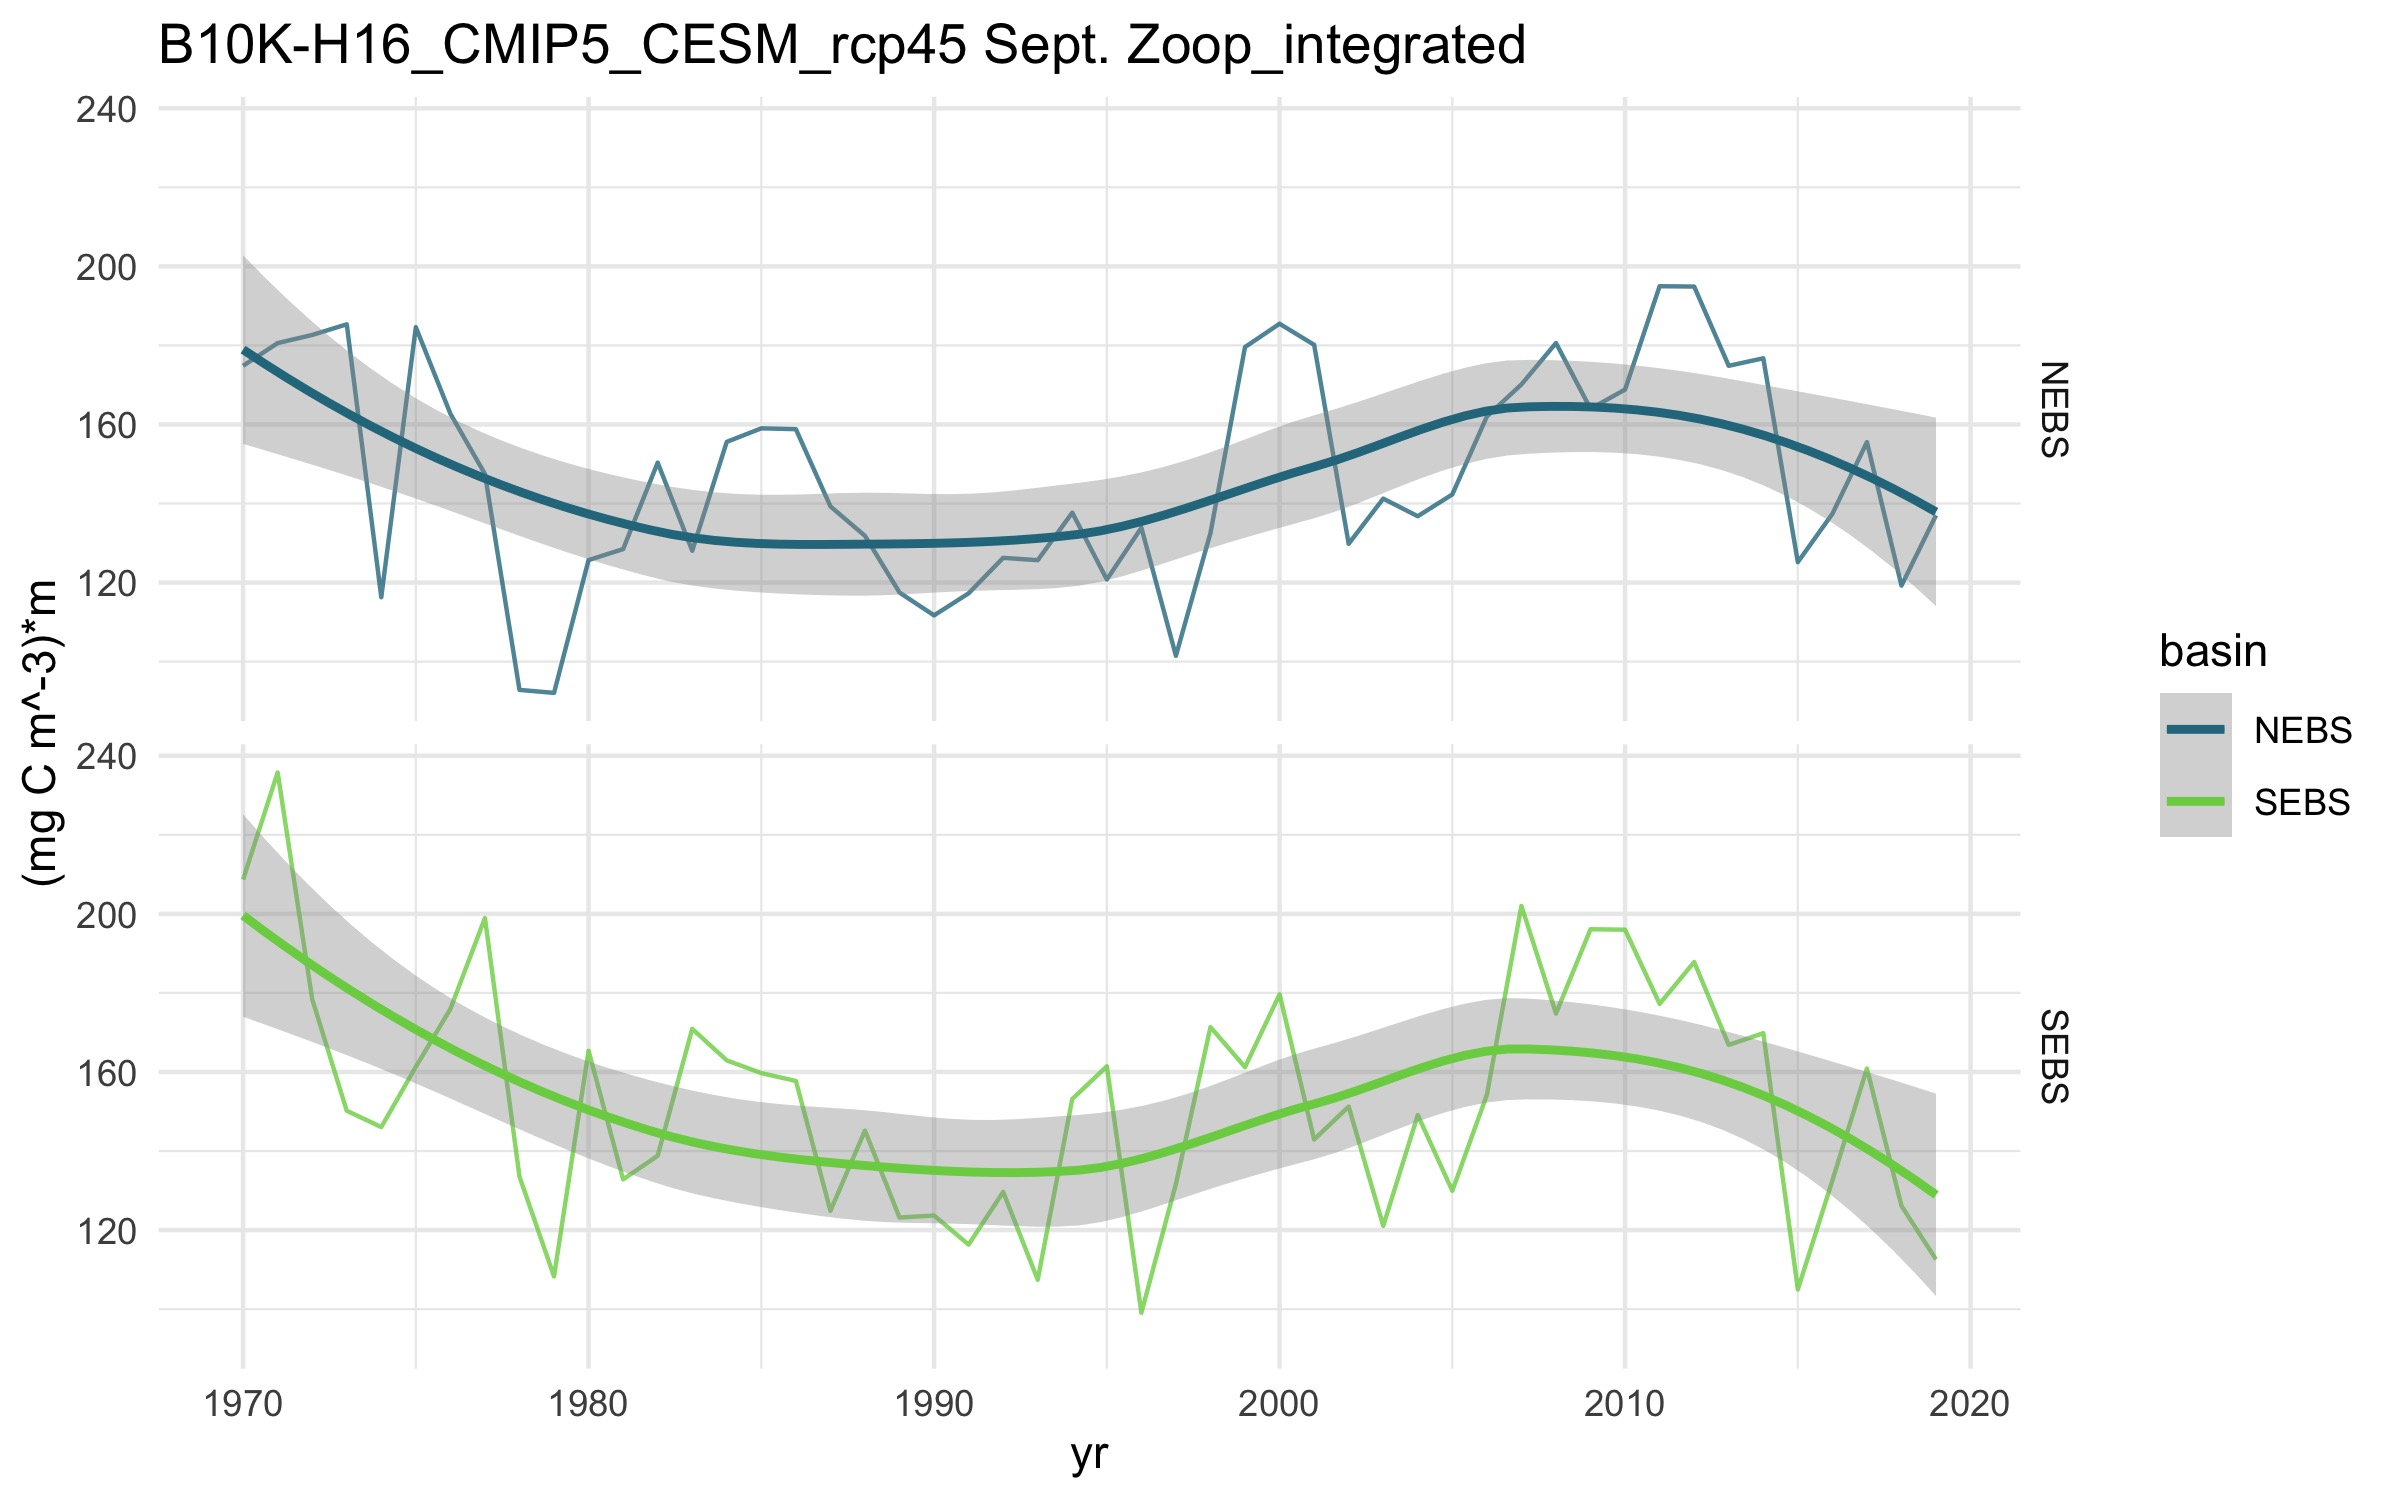
\includegraphics[width=0.65\textwidth,height=\textheight]{Figs/Hind_Sept_large_Zoop.jpg}
\#\# 5.2. Level 2 hindcasts

Level 2 data can be explored in the same way as the above indices but we
will focus in the section below on a simple spatial plot and temporal
index. The advantage of Level2 inidces is in the spatial resolution and
values outside of the survey area.

\hypertarget{level-2-hindcasts-custom-spatial-indices}{%
\subsubsection{5.2.1. Level 2 hindcasts: Custom spatial
indices}\label{level-2-hindcasts-custom-spatial-indices}}

As we did in section 5.1.1. let's create spatial plots of hindcast time
periods.

\begin{Shaded}
\begin{Highlighting}[]
   \CommentTok{# run this line if load_gis is set to F in R/setup.R:}
    \KeywordTok{source}\NormalTok{(}\StringTok{"R/sub_scripts/load_maps.R"}\NormalTok{)  }

    \CommentTok{# now create plots of average BT during four time periods}
\NormalTok{    time_seg   <-}\StringTok{ }\KeywordTok{list}\NormalTok{( }\StringTok{'1970-1980'}\NormalTok{ =}\StringTok{ }\KeywordTok{c}\NormalTok{(}\DecValTok{1970}\OperatorTok{:}\DecValTok{1980}\NormalTok{),}
                        \StringTok{'1980-1990'}\NormalTok{ =}\StringTok{ }\KeywordTok{c}\NormalTok{(}\DecValTok{1980}\OperatorTok{:}\DecValTok{1990}\NormalTok{),}
                        \StringTok{'1990-2000'}\NormalTok{ =}\StringTok{ }\KeywordTok{c}\NormalTok{(}\DecValTok{1990}\OperatorTok{:}\DecValTok{2000}\NormalTok{),}
                        \StringTok{'2000-2010'}\NormalTok{ =}\StringTok{ }\KeywordTok{c}\NormalTok{(}\DecValTok{2000}\OperatorTok{:}\DecValTok{2010}\NormalTok{),}
                        \StringTok{'2010-2020'}\NormalTok{ =}\StringTok{ }\KeywordTok{c}\NormalTok{(}\DecValTok{2010}\OperatorTok{:}\DecValTok{2020}\NormalTok{))}
    
   
    \CommentTok{# assign the simulation to download}
    \CommentTok{# --> Tinker: try selecting a different set of models to compare}
\NormalTok{    sim        <-}\StringTok{ "B10K-K20_CORECFS"} 
    \CommentTok{#ms <- c("B10K-H16_CORECFS","B10K-K20_CORECFS" )}
   
\NormalTok{    svl <-}\StringTok{ }\KeywordTok{list}\NormalTok{(}
      \StringTok{'Bottom 5m'}\NormalTok{ =}\StringTok{ "temp"}\NormalTok{,}
      \StringTok{'Surface 5m'}\NormalTok{ =}\StringTok{ "temp"}\NormalTok{,}
      \StringTok{'Integrated'}\NormalTok{ =}\StringTok{ }\KeywordTok{c}\NormalTok{(}\StringTok{"EupS"}\NormalTok{,}\StringTok{"Cop"}\NormalTok{,}\StringTok{"NCaS"}\NormalTok{) ) }
   
    \CommentTok{# Currently available Level 2 variables}
\NormalTok{    dl     <-}\StringTok{ }\NormalTok{proj_l2_datasets}\OperatorTok{$}\NormalTok{dataset  }\CommentTok{# datasets}
   
    
    \CommentTok{# Let's sample the model years as close to Aug 1 as the model timesteps run:}
\NormalTok{    tr          <-}\StringTok{ }\KeywordTok{c}\NormalTok{(}\StringTok{"-08-1 12:00:00 GMT"}\NormalTok{) }
    
    \CommentTok{# the full grid is large and takes a longtime to plot, so let's subsample the grid every 4 cells}
   
\NormalTok{    IDin       <-}\StringTok{ "_Aug1_subgrid"}
\NormalTok{    var_use    <-}\StringTok{ "_bottom5m_temp"}
    
    \CommentTok{# open a "region" or strata specific nc file}
\NormalTok{    fl         <-}\StringTok{ }\KeywordTok{file.path}\NormalTok{(main,Rdata_path,sim,}\StringTok{"Level2"}\NormalTok{,}
                            \KeywordTok{paste0}\NormalTok{(sim,var_use,IDin,}\StringTok{".Rdata"}\NormalTok{))}
    
    \CommentTok{# load object 'ACLIMsurveyrep'}
    \ControlFlowTok{if}\NormalTok{(}\OperatorTok{!}\KeywordTok{file.exists}\NormalTok{(}\KeywordTok{file.path}\NormalTok{(Rdata_path,fl)))}
      \KeywordTok{get_l2}\NormalTok{(}
        \DataTypeTok{ID          =}\NormalTok{ IDin,}
        \DataTypeTok{xi_rangeIN  =} \KeywordTok{seq}\NormalTok{(}\DecValTok{1}\NormalTok{,}\DecValTok{182}\NormalTok{,}\DecValTok{10}\NormalTok{),}
        \DataTypeTok{eta_rangeIN =} \KeywordTok{seq}\NormalTok{(}\DecValTok{1}\NormalTok{,}\DecValTok{258}\NormalTok{,}\DecValTok{10}\NormalTok{),}
        \DataTypeTok{ds_list     =}\NormalTok{ dl,}
        \DataTypeTok{trIN        =}\NormalTok{ tr,}
        \DataTypeTok{sub_varlist =}\NormalTok{ svl,  }
        \DataTypeTok{sim_list    =}\NormalTok{ sim  )}
    
    \CommentTok{# load R data file}
    \KeywordTok{load}\NormalTok{(fl)   }\CommentTok{# temp}
    
    \CommentTok{# there are smarter ways to do this;looping because }
    \CommentTok{# we don't want to mess it up but this is slow...}
\NormalTok{    i <-}\DecValTok{1}
\NormalTok{    data_long <-}\StringTok{ }\KeywordTok{data.frame}\NormalTok{(}\DataTypeTok{latitude =} \KeywordTok{as.vector}\NormalTok{(temp}\OperatorTok{$}\NormalTok{lat),}
                       \DataTypeTok{longitude =} \KeywordTok{as.vector}\NormalTok{(temp}\OperatorTok{$}\NormalTok{lon),}
                       \DataTypeTok{val =} \KeywordTok{as.vector}\NormalTok{(temp}\OperatorTok{$}\NormalTok{val[,,i]),}
                       \DataTypeTok{time =}\NormalTok{ temp}\OperatorTok{$}\NormalTok{time[i],}
                       \DataTypeTok{year =} \KeywordTok{substr}\NormalTok{( temp}\OperatorTok{$}\NormalTok{time[i],}\DecValTok{1}\NormalTok{,}\DecValTok{4}\NormalTok{),}\DataTypeTok{stringsAsFactors =}\NormalTok{ F}
\NormalTok{                       )}
    \ControlFlowTok{for}\NormalTok{(i }\ControlFlowTok{in} \DecValTok{2}\OperatorTok{:}\KeywordTok{dim}\NormalTok{(temp}\OperatorTok{$}\NormalTok{val)[}\DecValTok{3}\NormalTok{])}
\NormalTok{      data_long <-}\StringTok{ }\KeywordTok{rbind}\NormalTok{(data_long,}
                          \KeywordTok{data.frame}\NormalTok{(}\DataTypeTok{latitude =} \KeywordTok{as.vector}\NormalTok{(temp}\OperatorTok{$}\NormalTok{lat),}
                           \DataTypeTok{longitude =} \KeywordTok{as.vector}\NormalTok{(temp}\OperatorTok{$}\NormalTok{lon),}
                           \DataTypeTok{val =} \KeywordTok{as.vector}\NormalTok{(temp}\OperatorTok{$}\NormalTok{val[,,i]),}
                           \DataTypeTok{time =}\NormalTok{ temp}\OperatorTok{$}\NormalTok{time[i],}
                           \DataTypeTok{year =} \KeywordTok{substr}\NormalTok{( temp}\OperatorTok{$}\NormalTok{time[i],}\DecValTok{1}\NormalTok{,}\DecValTok{4}\NormalTok{),}\DataTypeTok{stringsAsFactors =}\NormalTok{ F)}
\NormalTok{                       )}
    
    
    \CommentTok{# get the mean values for the time blocks from the rdata versions}
    \CommentTok{# will throw "implicit NA" errors that can be ignored}
\NormalTok{    tmp_var <-data_long }\CommentTok{# get mean var val for each time segment}
\NormalTok{    j<-}\DecValTok{0}
    \ControlFlowTok{for}\NormalTok{(i }\ControlFlowTok{in} \DecValTok{1}\OperatorTok{:}\KeywordTok{length}\NormalTok{(time_seg))\{}
      \ControlFlowTok{if}\NormalTok{(}\KeywordTok{length}\NormalTok{( }\KeywordTok{which}\NormalTok{(}\KeywordTok{as.numeric}\NormalTok{(tmp_var}\OperatorTok{$}\NormalTok{year)}\OperatorTok\NormalTok{time_seg[[i]] ))}\OperatorTok{>}\DecValTok{0}\NormalTok{)\{}
\NormalTok{        j <-}\StringTok{ }\NormalTok{j }\OperatorTok{+}\DecValTok{1}
\NormalTok{         mn_tmp_var <-}\StringTok{ }\NormalTok{tmp_var}\OperatorTok
\StringTok{          }\KeywordTok{filter}\NormalTok{(year}\OperatorTok\NormalTok{time_seg[[i]],}\OperatorTok{!}\KeywordTok{is.na}\NormalTok{(val))}\OperatorTok
\StringTok{          }\KeywordTok{group_by}\NormalTok{(latitude, longitude)}\OperatorTok
\StringTok{          }\KeywordTok{summarise}\NormalTok{(}\DataTypeTok{mnval =} \KeywordTok{mean}\NormalTok{(val,}\DataTypeTok{rm.na=}\NormalTok{T))}
        
\NormalTok{        mn_tmp_var}\OperatorTok{$}\NormalTok{time_period =}\StringTok{ }\KeywordTok{factor}\NormalTok{(}\KeywordTok{names}\NormalTok{(time_seg)[i],}\DataTypeTok{levels=}\KeywordTok{names}\NormalTok{(time_seg))}
      \ControlFlowTok{if}\NormalTok{(j }\OperatorTok{==}\StringTok{ }\DecValTok{1}\NormalTok{) mn_var <-}\StringTok{ }\NormalTok{mn_tmp_var}
      \ControlFlowTok{if}\NormalTok{(j }\OperatorTok{>}\StringTok{  }\DecValTok{1}\NormalTok{) mn_var <-}\StringTok{ }\KeywordTok{rbind}\NormalTok{(mn_var,mn_tmp_var)}
       \KeywordTok{rm}\NormalTok{(mn_tmp_var)}
\NormalTok{      \}}
\NormalTok{    \}}
    
    \CommentTok{# convert results to a shapefile}
\NormalTok{    L2_sf  <-}\StringTok{ }\KeywordTok{convert2shp}\NormalTok{(mn_var}\OperatorTok\KeywordTok{filter}\NormalTok{(}\OperatorTok{!}\KeywordTok{is.na}\NormalTok{(mnval)))}
    
\NormalTok{    p9     <-}\StringTok{ }\KeywordTok{plot_stations_basemap}\NormalTok{(}\DataTypeTok{sfIN =}\NormalTok{ L2_sf,}
                                \DataTypeTok{fillIN =} \StringTok{"mnval"}\NormalTok{,}
                                \DataTypeTok{colorIN =} \StringTok{"mnval"}\NormalTok{,}
                                \DataTypeTok{sizeIN=}\NormalTok{.}\DecValTok{6}\NormalTok{) }\OperatorTok{+}
\StringTok{      }\KeywordTok{facet_grid}\NormalTok{(.}\OperatorTok{~}\NormalTok{time_period)}\OperatorTok{+}
\StringTok{      }\KeywordTok{scale_color_viridis_c}\NormalTok{()}\OperatorTok{+}
\StringTok{      }\KeywordTok{scale_fill_viridis_c}\NormalTok{()}\OperatorTok{+}
\StringTok{      }\KeywordTok{guides}\NormalTok{(}
        \DataTypeTok{color =}  \KeywordTok{guide_legend}\NormalTok{(}\DataTypeTok{title=}\StringTok{"Bottom T (degC)"}\NormalTok{),}
        \DataTypeTok{fill  =}  \KeywordTok{guide_legend}\NormalTok{(}\DataTypeTok{title=}\StringTok{"Bottom T (degC)"}\NormalTok{)) }\OperatorTok{+}
\StringTok{      }\KeywordTok{ggtitle}\NormalTok{(}\KeywordTok{paste}\NormalTok{(sim,var_use,IDin))}
   
    \CommentTok{# This is slow but it works (repeat dev.new() twice if in Rstudio)...}
    \KeywordTok{dev.new}\NormalTok{()}
\NormalTok{    p9}
    
    \ControlFlowTok{if}\NormalTok{(update.figs)  }\KeywordTok{ggsave}\NormalTok{(}\DataTypeTok{file=}\KeywordTok{file.path}\NormalTok{(main,}\StringTok{"Figs/sub_grid_mn_BT_Aug1.jpg"}\NormalTok{),}\DataTypeTok{width=}\DecValTok{8}\NormalTok{,}\DataTypeTok{height=}\DecValTok{6}\NormalTok{)}
  
    \CommentTok{# graphics.off()}
\end{Highlighting}
\end{Shaded}

\begin{figure}
\centering
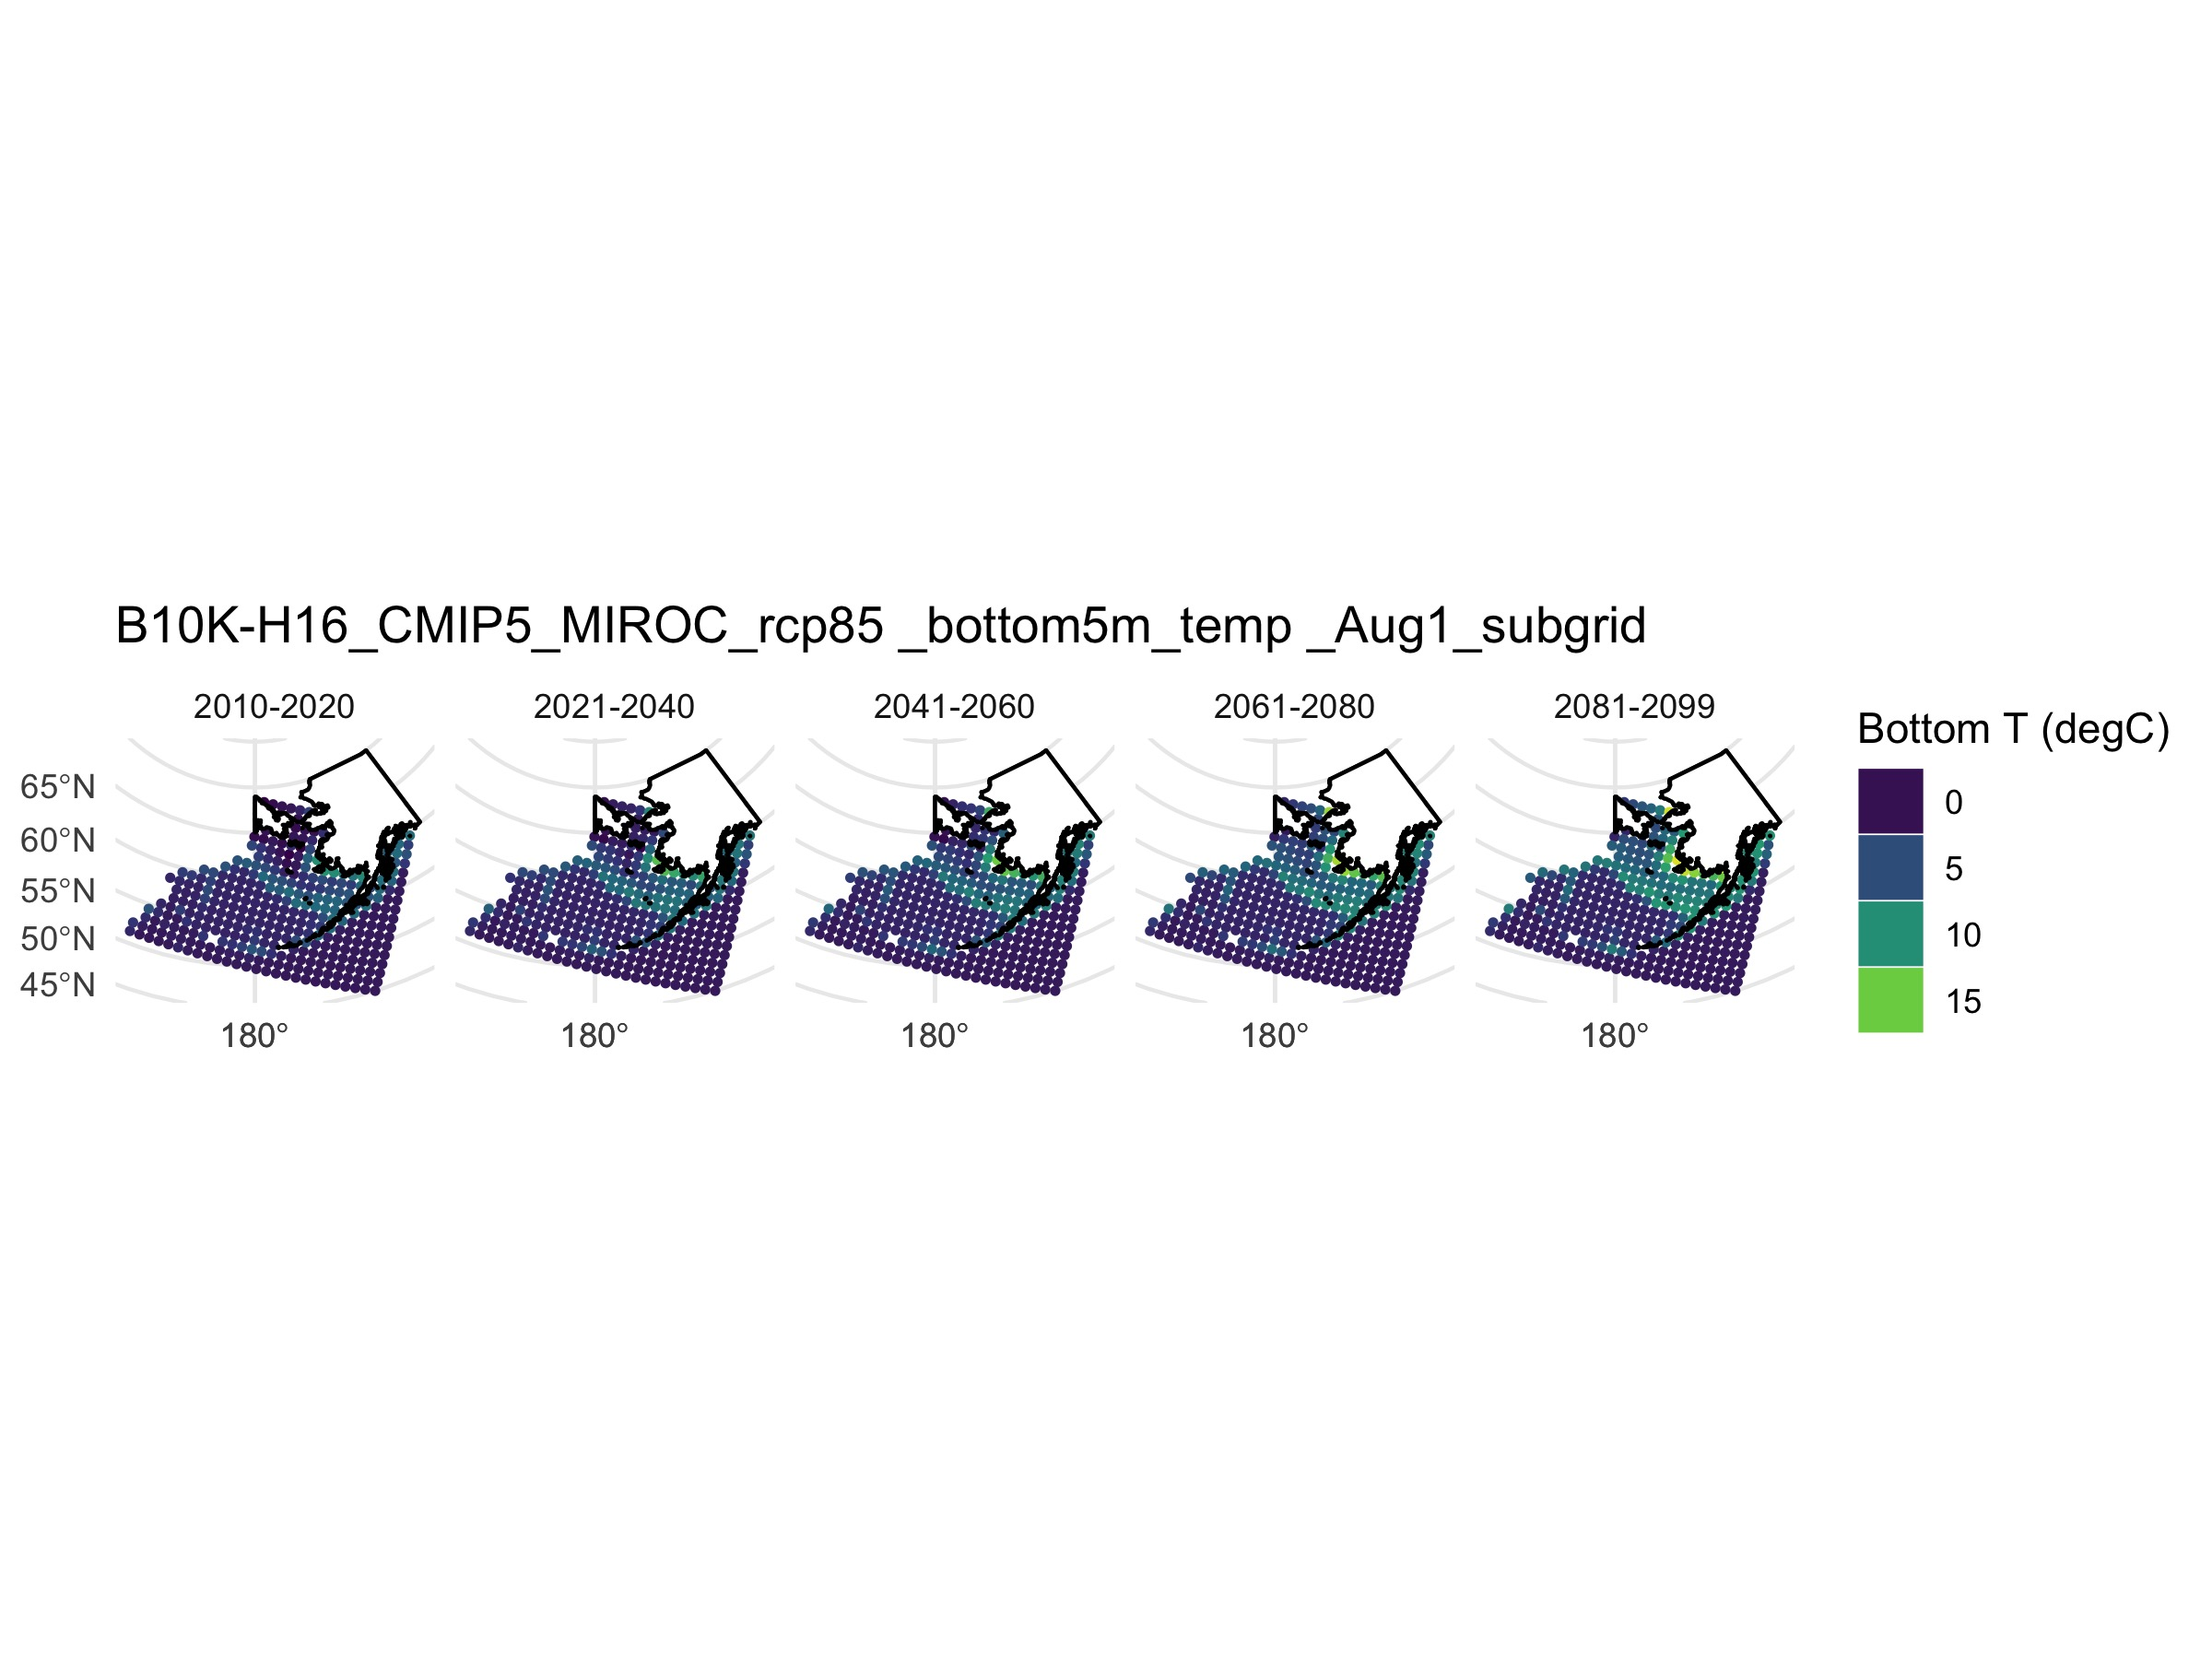
\includegraphics[width=0.65\textwidth,height=\textheight]{Figs/sub_grid_mn_BT_Aug1.jpg}
\caption{Aug 1 Bottom temperature from Level 2 dataset}
\end{figure}

\hypertarget{level-2-hindcasts-m2-mooring-comparison}{%
\subsubsection{5.2.2. Level 2 hindcasts: M2 mooring
comparison}\label{level-2-hindcasts-m2-mooring-comparison}}

\hypertarget{projections}{%
\section{6. Projections:}\label{projections}}

The ACLIM project utilizes the full ``suite'' of Bering10K model
hindcasts and projections, summarized in the following table. These
represent downscaled models hindcast and projections based whereby
boundary conditions of the high resolution Bering10K model are forced by
the coarser resolution General Circulation Models (GCM) run under
Coupled Model Intercomparison Project (CMIP) phase 5 (5th IPCC
Assessment Report) or phase 6 (6th IPCC Assessment Report; ``AR'')
global carbon mitigation scenarios. Hindcasts are similarly forced at
the boundaries from global scale climate reanalysis CORE and CFS
products. For full details see the Kearney 2021 Tech. Memo.

\hypertarget{table-1-summary-of-romsnpz-downscaled-model-runs}{%
\subsection{Table 1: Summary of ROMSNPZ downscaled model
runs}\label{table-1-summary-of-romsnpz-downscaled-model-runs}}

\begin{longtable}[]{@{}lllllllll@{}}
\toprule
CMIP & GCM & Scenario & Def & Years & Model & Source & Status
&\tabularnewline
\midrule
\endhead
& CORECFS & Reanalysis & Hindcast & 1970 - 2018 & H16 & IEA/ACLIM &
Public &\tabularnewline
& CORECFS & Reanalysis & Hindcast & 1970 - 2020 & K20 & MAPP/IEA/ACLIM &
Public &\tabularnewline
5 & GFDL & RCP 4.5 & Med. mitigation & 2006 - 2099 & H16 & ACLIM/FATE &
Public &\tabularnewline
5 & GFDL & RCP 8.5 & High baseline & 2006 - 2099 & H16 & ACLIM/FATE &
Public &\tabularnewline
5 & GFDL & RCP 8.5bio* & High baseline & 2006 - 2099 & H16 & ACLIM/FATE
& Public &\tabularnewline
5 & MIROC & RCP 4.5 & Med. mitigation & 2006 - 2099 & H16 & ACLIM/FATE &
Public &\tabularnewline
5 & MIROC & RCP 8.5 & High baseline & 2006 - 2099 & H16 & ACLIM/FATE &
Public &\tabularnewline
5 & CESM & RCP 4.5 & Med. mitigation & 2006 - 2099 & H16 & ACLIM/FATE &
Public &\tabularnewline
5 & CESM & RCP 8.5 & High baseline & 2006 - 2080 & H16 & ACLIM/FATE &
Public &\tabularnewline
5 & CESM & RCP 8.5bio* & High baseline & 2006 - 2099 & H16 & ACLIM/FATE
& Public &\tabularnewline
6 & CESM & SSP585 & High baseline & 2014 - 2099 & K20P19 & ACLIM2/RTAP &
Embargo &\tabularnewline
6 & CESM & SSP126 & High Mitigation & 2014 - 2099 & K20P19 & ACLIM2/RTAP
& Embargo &\tabularnewline
6 & CESM & Historical & Historical & 1980 - 2014 & K20P19 & ACLIM2/RTAP
& Embargo &\tabularnewline
6 & GFDL & SSP585 & High baseline & 2014 - 2099 & K20P19 & ACLIM2/RTAP &
Embargo &\tabularnewline
6 & GFDL & SSP126 & High Mitigation & 2014 - 2099 & K20P19 & ACLIM2/RTAP
& Embargo &\tabularnewline
6 & GFDL & Historical & Historical & 1980 - 2014 & K20P19 & ACLIM2/RTAP
& Embargo &\tabularnewline
6 & MIROC & SSP585 & High baseline & 2014 - 2099 & K20P19 & ACLIM2/RTAP
& Embargo &\tabularnewline
6 & MIROC & SSP126 & High Mitigation & 2014 - 2099 & K20P19 &
ACLIM2/RTAP & Embargo &\tabularnewline
6 & MIROC & Historical & Historical & 1980 - 2014 & K20P19 & ACLIM2/RTAP
& Embargo &\tabularnewline
\bottomrule
\end{longtable}

*``bio'' = nutrient forcing on boundary conditions

\hypertarget{level-3-projections}{%
\subsection{6.1. Level 3 projections}\label{level-3-projections}}

some text here

\hypertarget{level-3-projections-spatial-patterns}{%
\subsubsection{6.1.1. Level 3 projections: spatial
patterns}\label{level-3-projections-spatial-patterns}}

Now let's explore the survey replicated data in more detail and use to
plot bottom temperature.

\begin{Shaded}
\begin{Highlighting}[]
    \CommentTok{# now create plots of average BT during four time periods}
\NormalTok{    time_seg   <-}\StringTok{ }\KeywordTok{list}\NormalTok{( }\StringTok{'2010-2020'}\NormalTok{ =}\StringTok{ }\KeywordTok{c}\NormalTok{(}\DecValTok{2010}\OperatorTok{:}\DecValTok{2020}\NormalTok{),}
                        \StringTok{'2021-2040'}\NormalTok{ =}\StringTok{ }\KeywordTok{c}\NormalTok{(}\DecValTok{2021}\OperatorTok{:}\DecValTok{2040}\NormalTok{),}
                        \StringTok{'2041-2060'}\NormalTok{ =}\StringTok{ }\KeywordTok{c}\NormalTok{(}\DecValTok{2041}\OperatorTok{:}\DecValTok{2060}\NormalTok{),}
                        \StringTok{'2061-2080'}\NormalTok{ =}\StringTok{ }\KeywordTok{c}\NormalTok{(}\DecValTok{2061}\OperatorTok{:}\DecValTok{2080}\NormalTok{),}
                        \StringTok{'2081-2099'}\NormalTok{ =}\StringTok{ }\KeywordTok{c}\NormalTok{(}\DecValTok{2081}\OperatorTok{:}\DecValTok{2099}\NormalTok{))}
    
    \CommentTok{# lists the possible variables}
\NormalTok{    srvy_vars}
    
    \CommentTok{# specify the variables to plot}
\NormalTok{    vl        <-}\StringTok{ }\KeywordTok{c}\NormalTok{(}
                  \StringTok{"temp_bottom5m"}\NormalTok{,}
                  \StringTok{"NCaS_integrated"}\NormalTok{, }\CommentTok{# Large Cop}
                  \StringTok{"Cop_integrated"}\NormalTok{,  }\CommentTok{# Small Cop}
                  \StringTok{"EupS_integrated"}\NormalTok{) }\CommentTok{# Euphausiids}
    
    \CommentTok{# View possible simulations:}
    \KeywordTok{head}\NormalTok{(aclim)}
    
    \CommentTok{# assign the simulation to download}
    \CommentTok{# --> Tinker: try selecting a different set of models to compare}
\NormalTok{    sim        <-}\StringTok{"B10K-H16_CMIP5_MIROC_rcp85"} 
    
    \CommentTok{# open a "region" or strata specific nc file}
\NormalTok{    fl         <-}\StringTok{ }\KeywordTok{file.path}\NormalTok{(sim,}\KeywordTok{paste0}\NormalTok{(srvy_txt,sim,}\StringTok{".Rdata"}\NormalTok{))}
    
    \CommentTok{# load object 'ACLIMsurveyrep'}
    \KeywordTok{load}\NormalTok{(}\KeywordTok{file.path}\NormalTok{(main,Rdata_path,fl))   }
     
    \CommentTok{# create local rdata files }
    \ControlFlowTok{if}\NormalTok{(}\OperatorTok{!}\KeywordTok{file.exists}\NormalTok{(}\KeywordTok{file.path}\NormalTok{(Rdata_path,fl)))}
      \KeywordTok{get_l3}\NormalTok{(}\DataTypeTok{web_nc =} \OtherTok{TRUE}\NormalTok{, }\DataTypeTok{download_nc =}\NormalTok{ F,}
          \DataTypeTok{varlist =}\NormalTok{ vl,}\DataTypeTok{sim_list =}\NormalTok{sim )}
    
    
     \CommentTok{# Collate mean values across timeperiods and simulations}
    \CommentTok{# -------------------------------------------------------}
\NormalTok{    m_set      <-}\StringTok{ }\KeywordTok{c}\NormalTok{(}\DecValTok{9}\NormalTok{,}\DecValTok{7}\NormalTok{,}\DecValTok{8}\NormalTok{)}
\NormalTok{    ms         <-}\StringTok{ }\NormalTok{aclim[m_set]}
    
    \CommentTok{# Loop over model set}
    \ControlFlowTok{for}\NormalTok{(sim }\ControlFlowTok{in}\NormalTok{ ms)\{}
\NormalTok{     fl         <-}\StringTok{ }\KeywordTok{file.path}\NormalTok{(sim,}\KeywordTok{paste0}\NormalTok{(srvy_txt,sim,}\StringTok{".Rdata"}\NormalTok{))}
    
    \CommentTok{# download & convert .nc files that are not already in Rdata folder}
    \ControlFlowTok{if}\NormalTok{(}\OperatorTok{!}\KeywordTok{file.exists}\NormalTok{( }\KeywordTok{file.path}\NormalTok{(Rdata_path,fl)) )}
      \KeywordTok{get_l3}\NormalTok{(}\DataTypeTok{web_nc =} \OtherTok{TRUE}\NormalTok{, }\DataTypeTok{download_nc =}\NormalTok{ F,}
          \DataTypeTok{varlist =}\NormalTok{ vl,}\DataTypeTok{sim_list =}\NormalTok{sim )}
\NormalTok{    \}}
      
    \CommentTok{# get the mean values for the time blocks from the rdata versions}
    \CommentTok{# will throw "implicit NA" errors that can be ignored}
\NormalTok{    mn_var_all <-}\StringTok{ }\KeywordTok{get_mn_rd}\NormalTok{(}\DataTypeTok{modset =}\NormalTok{ ms ,}\DataTypeTok{varUSE=}\StringTok{"temp_bottom5m"}\NormalTok{)}
    
    \CommentTok{# convert results to a shapefile}
\NormalTok{    mn_var_sf  <-}\StringTok{ }\KeywordTok{convert2shp}\NormalTok{(mn_var_all}\OperatorTok\KeywordTok{filter}\NormalTok{(}\OperatorTok{!}\KeywordTok{is.na}\NormalTok{(mnval)))}
\NormalTok{    lab_t      <-}\StringTok{ }\NormalTok{ms[}\DecValTok{2}\NormalTok{]}\OperatorTok\NormalTok{stringr}\OperatorTok{::}\KeywordTok{str_remove}\NormalTok{(}\StringTok{"([^-])"}\NormalTok{)}
    
\NormalTok{    p3         <-}\StringTok{ }\KeywordTok{plot_stations_basemap}\NormalTok{(}\DataTypeTok{sfIN =}\NormalTok{ mn_var_sf,}
                                \DataTypeTok{fillIN =} \StringTok{"mnval"}\NormalTok{,}
                                \DataTypeTok{colorIN =} \StringTok{"mnval"}\NormalTok{,}
                                \DataTypeTok{sizeIN=}\NormalTok{.}\DecValTok{3}\NormalTok{) }\OperatorTok{+}
\StringTok{      }\KeywordTok{facet_grid}\NormalTok{(simulation}\OperatorTok{~}\NormalTok{time_period)}\OperatorTok{+}
\StringTok{      }\KeywordTok{scale_color_viridis_c}\NormalTok{()}\OperatorTok{+}
\StringTok{      }\KeywordTok{scale_fill_viridis_c}\NormalTok{()}\OperatorTok{+}
\StringTok{      }\KeywordTok{guides}\NormalTok{(}
        \DataTypeTok{color =}  \KeywordTok{guide_legend}\NormalTok{(}\DataTypeTok{title=}\StringTok{"Bottom T (degC)"}\NormalTok{),}
        \DataTypeTok{fill  =}  \KeywordTok{guide_legend}\NormalTok{(}\DataTypeTok{title=}\StringTok{"Bottom T (degC)"}\NormalTok{)) }\OperatorTok{+}
\StringTok{      }\KeywordTok{ggtitle}\NormalTok{(lab_t)}
   
    \CommentTok{# This is slow but it works (repeat dev.new() twice if in Rstudio)...}
    \KeywordTok{dev.new}\NormalTok{()}
\NormalTok{    p3}
    
    \ControlFlowTok{if}\NormalTok{(update.figs)  }\KeywordTok{ggsave}\NormalTok{(}\DataTypeTok{file=}\KeywordTok{file.path}\NormalTok{(main,}\StringTok{"Figs/mn_BT.jpg"}\NormalTok{),}\DataTypeTok{width=}\DecValTok{8}\NormalTok{,}\DataTypeTok{height=}\DecValTok{6}\NormalTok{)}
  
    \CommentTok{# graphics.off()}
\end{Highlighting}
\end{Shaded}

\begin{figure}
\centering
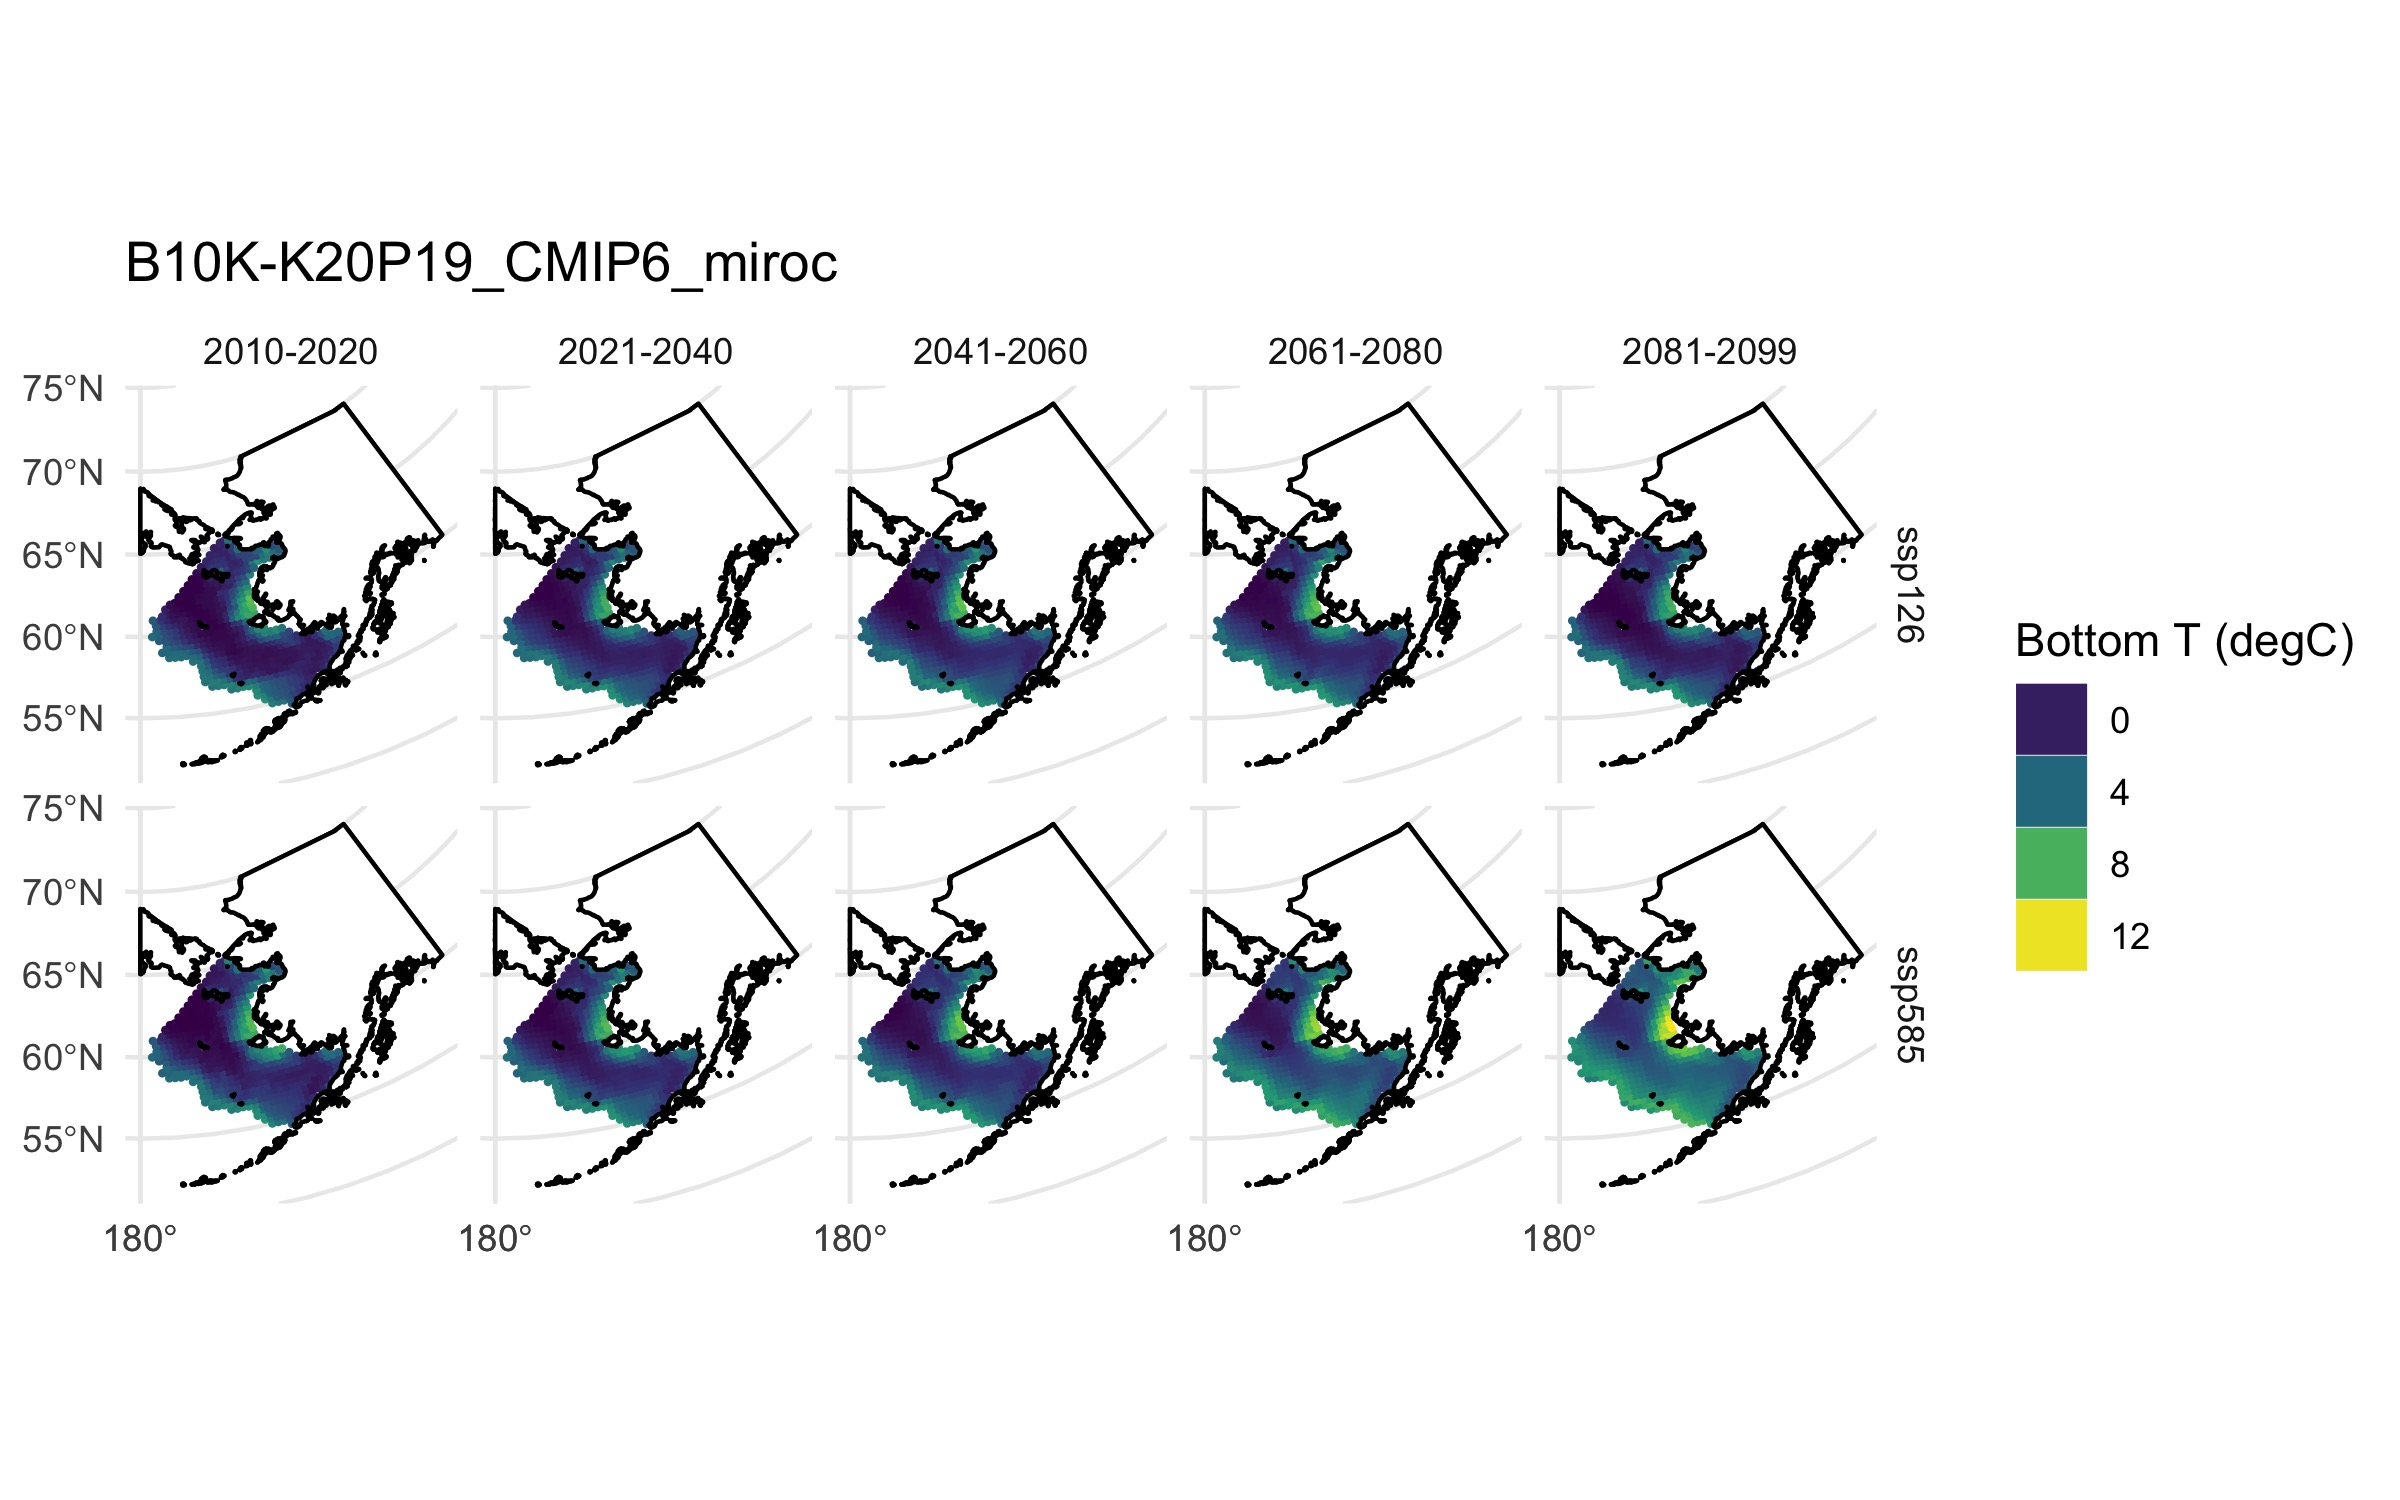
\includegraphics{Figs/mn_BT.jpg}
\caption{Bottom temperature projections under differing SSP126 (top row)
and SSP585 (bottom row)}
\end{figure}

\hypertarget{level-3-projections-weekly-strata-averages}{%
\subsubsection{6.1.2. Level 3 projections: Weekly strata
averages}\label{level-3-projections-weekly-strata-averages}}

The next set of indices to will explore are the weekly strata-specific
values for each variable.These are stored in the
\texttt{ACLIMregion\_B10K-{[}version\_CMIPx\_GCM\_RCP{]}.nc} in each
scenario folder.

\begin{Shaded}
\begin{Highlighting}[]
    \CommentTok{# View an individual variable (e.g., Bottom Temp)}
    \CommentTok{# -------------------------------------------------------}
\NormalTok{    weekly_vars}
\NormalTok{    aclim}
\NormalTok{    sim        <-}\StringTok{"B10K-H16_CMIP5_MIROC_rcp85"} 
    
    \CommentTok{# open a "region" or strata specific nc file}
\NormalTok{    fl         <-}\StringTok{ }\KeywordTok{file.path}\NormalTok{(sim,}\KeywordTok{paste0}\NormalTok{(reg_txt,sim,}\StringTok{".Rdata"}\NormalTok{))}
    
\NormalTok{    var_use   <-}\StringTok{ "temp_bottom5m"}
\NormalTok{    vl        <-}\StringTok{ }\KeywordTok{c}\NormalTok{(}
                  \StringTok{"temp_bottom5m"}\NormalTok{,}
                  \StringTok{"NCaS_integrated"}\NormalTok{, }\CommentTok{# Large Cop}
                  \StringTok{"Cop_integrated"}\NormalTok{,  }\CommentTok{# Small Cop}
                  \StringTok{"EupS_integrated"}\NormalTok{) }\CommentTok{# Euphausiids}
    
    \CommentTok{# create local rdata files (opt 1)}
    \ControlFlowTok{if}\NormalTok{(}\OperatorTok{!}\KeywordTok{file.exists}\NormalTok{(}\KeywordTok{file.path}\NormalTok{(Rdata_path,fl)))}
      \KeywordTok{get_l3}\NormalTok{(}\DataTypeTok{web_nc =} \OtherTok{TRUE}\NormalTok{, }\DataTypeTok{download_nc =}\NormalTok{ F,}
          \DataTypeTok{varlist =}\NormalTok{ vl,}\DataTypeTok{sim_list =}\NormalTok{ sim)}
    
    \CommentTok{# load object 'ACLIMregion'}
    \KeywordTok{load}\NormalTok{(}\KeywordTok{file.path}\NormalTok{(main,Rdata_path,fl))  }
\NormalTok{    tmp_var    <-}\StringTok{ }\NormalTok{ACLIMregion}\OperatorTok\KeywordTok{filter}\NormalTok{(var }\OperatorTok{==}\StringTok{ }\NormalTok{var_use)}
    
   \CommentTok{# now plot the data:}
   
\NormalTok{   p4 <-}\StringTok{ }\KeywordTok{ggplot}\NormalTok{(}\DataTypeTok{data =}\NormalTok{ tmp_var) }\OperatorTok{+}\StringTok{ }
\StringTok{     }\KeywordTok{geom_line}\NormalTok{(}\KeywordTok{aes}\NormalTok{(}\DataTypeTok{x=}\NormalTok{time,}\DataTypeTok{y=}\NormalTok{val,}\DataTypeTok{color=}\NormalTok{ strata),}\DataTypeTok{alpha=}\NormalTok{.}\DecValTok{8}\NormalTok{)}\OperatorTok{+}
\StringTok{     }\KeywordTok{facet_grid}\NormalTok{(basin}\OperatorTok{~}\NormalTok{.)}\OperatorTok{+}
\StringTok{     }\KeywordTok{ylab}\NormalTok{(tmp_var}\OperatorTok{$}\NormalTok{units[}\DecValTok{1}\NormalTok{])}\OperatorTok{+}
\StringTok{     }\KeywordTok{ggtitle}\NormalTok{( }\KeywordTok{paste}\NormalTok{(sim,tmp_var}\OperatorTok{$}\NormalTok{var[}\DecValTok{1}\NormalTok{]))}\OperatorTok{+}
\StringTok{     }\KeywordTok{theme_minimal}\NormalTok{()}
\NormalTok{   p4}
    \ControlFlowTok{if}\NormalTok{(update.figs)  }\KeywordTok{ggsave}\NormalTok{(}\DataTypeTok{file=}\KeywordTok{file.path}\NormalTok{(main,}\StringTok{"Figs/weekly_bystrata.jpg"}\NormalTok{),}\DataTypeTok{width=}\DecValTok{8}\NormalTok{,}\DataTypeTok{height=}\DecValTok{5}\NormalTok{)}

   
   \CommentTok{# To get the average value for a set of strata, weight the val by the area:}
\NormalTok{   mn_NEBS <-}\StringTok{ }\KeywordTok{getAVGnSUM}\NormalTok{(}\DataTypeTok{strataIN =}\NormalTok{ NEBS_strata, }\DataTypeTok{dataIN =}\NormalTok{ tmp_var)}
\NormalTok{   mn_NEBS}\OperatorTok{$}\NormalTok{basin =}\StringTok{ "NEBS"}
\NormalTok{   mn_SEBS <-}\KeywordTok{getAVGnSUM}\NormalTok{(}\DataTypeTok{strataIN =}\NormalTok{ SEBS_strata, }\DataTypeTok{dataIN =}\NormalTok{ tmp_var)}
\NormalTok{   mn_SEBS}\OperatorTok{$}\NormalTok{basin =}\StringTok{ "SEBS"}
   
\NormalTok{   p5 <-}\StringTok{ }\KeywordTok{ggplot}\NormalTok{(}\DataTypeTok{data =} \KeywordTok{rbind}\NormalTok{(mn_NEBS,mn_SEBS)) }\OperatorTok{+}\StringTok{ }
\StringTok{      }\KeywordTok{geom_line}\NormalTok{(}\KeywordTok{aes}\NormalTok{(}\DataTypeTok{x=}\NormalTok{time,}\DataTypeTok{y=}\NormalTok{mn_val,}\DataTypeTok{color=}\NormalTok{basin),}\DataTypeTok{alpha=}\NormalTok{.}\DecValTok{8}\NormalTok{)}\OperatorTok{+}
\StringTok{      }\KeywordTok{geom_smooth}\NormalTok{(}\KeywordTok{aes}\NormalTok{(}\DataTypeTok{x=}\NormalTok{time,}\DataTypeTok{y=}\NormalTok{mn_val,}\DataTypeTok{color=}\NormalTok{basin),}
                  \DataTypeTok{formula =}\NormalTok{ y }\OperatorTok{~}\StringTok{ }\NormalTok{x, }\DataTypeTok{se =}\NormalTok{ T)}\OperatorTok{+}
\StringTok{      }\KeywordTok{facet_grid}\NormalTok{(basin}\OperatorTok{~}\NormalTok{.)}\OperatorTok{+}
\StringTok{      }\KeywordTok{scale_color_viridis_d}\NormalTok{(}\DataTypeTok{begin=}\NormalTok{.}\DecValTok{4}\NormalTok{,}\DataTypeTok{end=}\NormalTok{.}\DecValTok{8}\NormalTok{)}\OperatorTok{+}
\StringTok{      }\KeywordTok{ylab}\NormalTok{(tmp_var}\OperatorTok{$}\NormalTok{units[}\DecValTok{1}\NormalTok{])}\OperatorTok{+}
\StringTok{      }\KeywordTok{ggtitle}\NormalTok{( }\KeywordTok{paste}\NormalTok{(sim,mn_NEBS}\OperatorTok{$}\NormalTok{var[}\DecValTok{1}\NormalTok{]))}\OperatorTok{+}
\StringTok{     }
\StringTok{      }\KeywordTok{theme_minimal}\NormalTok{()}
\NormalTok{  p5}
  \ControlFlowTok{if}\NormalTok{(update.figs)  }\KeywordTok{ggsave}\NormalTok{(}\DataTypeTok{file=}\KeywordTok{file.path}\NormalTok{(main,}\StringTok{"Figs/weekly_byreg.jpg"}\NormalTok{),}\DataTypeTok{width=}\DecValTok{8}\NormalTok{,}\DataTypeTok{height=}\DecValTok{5}\NormalTok{)}
\end{Highlighting}
\end{Shaded}

\begin{figure}
\centering
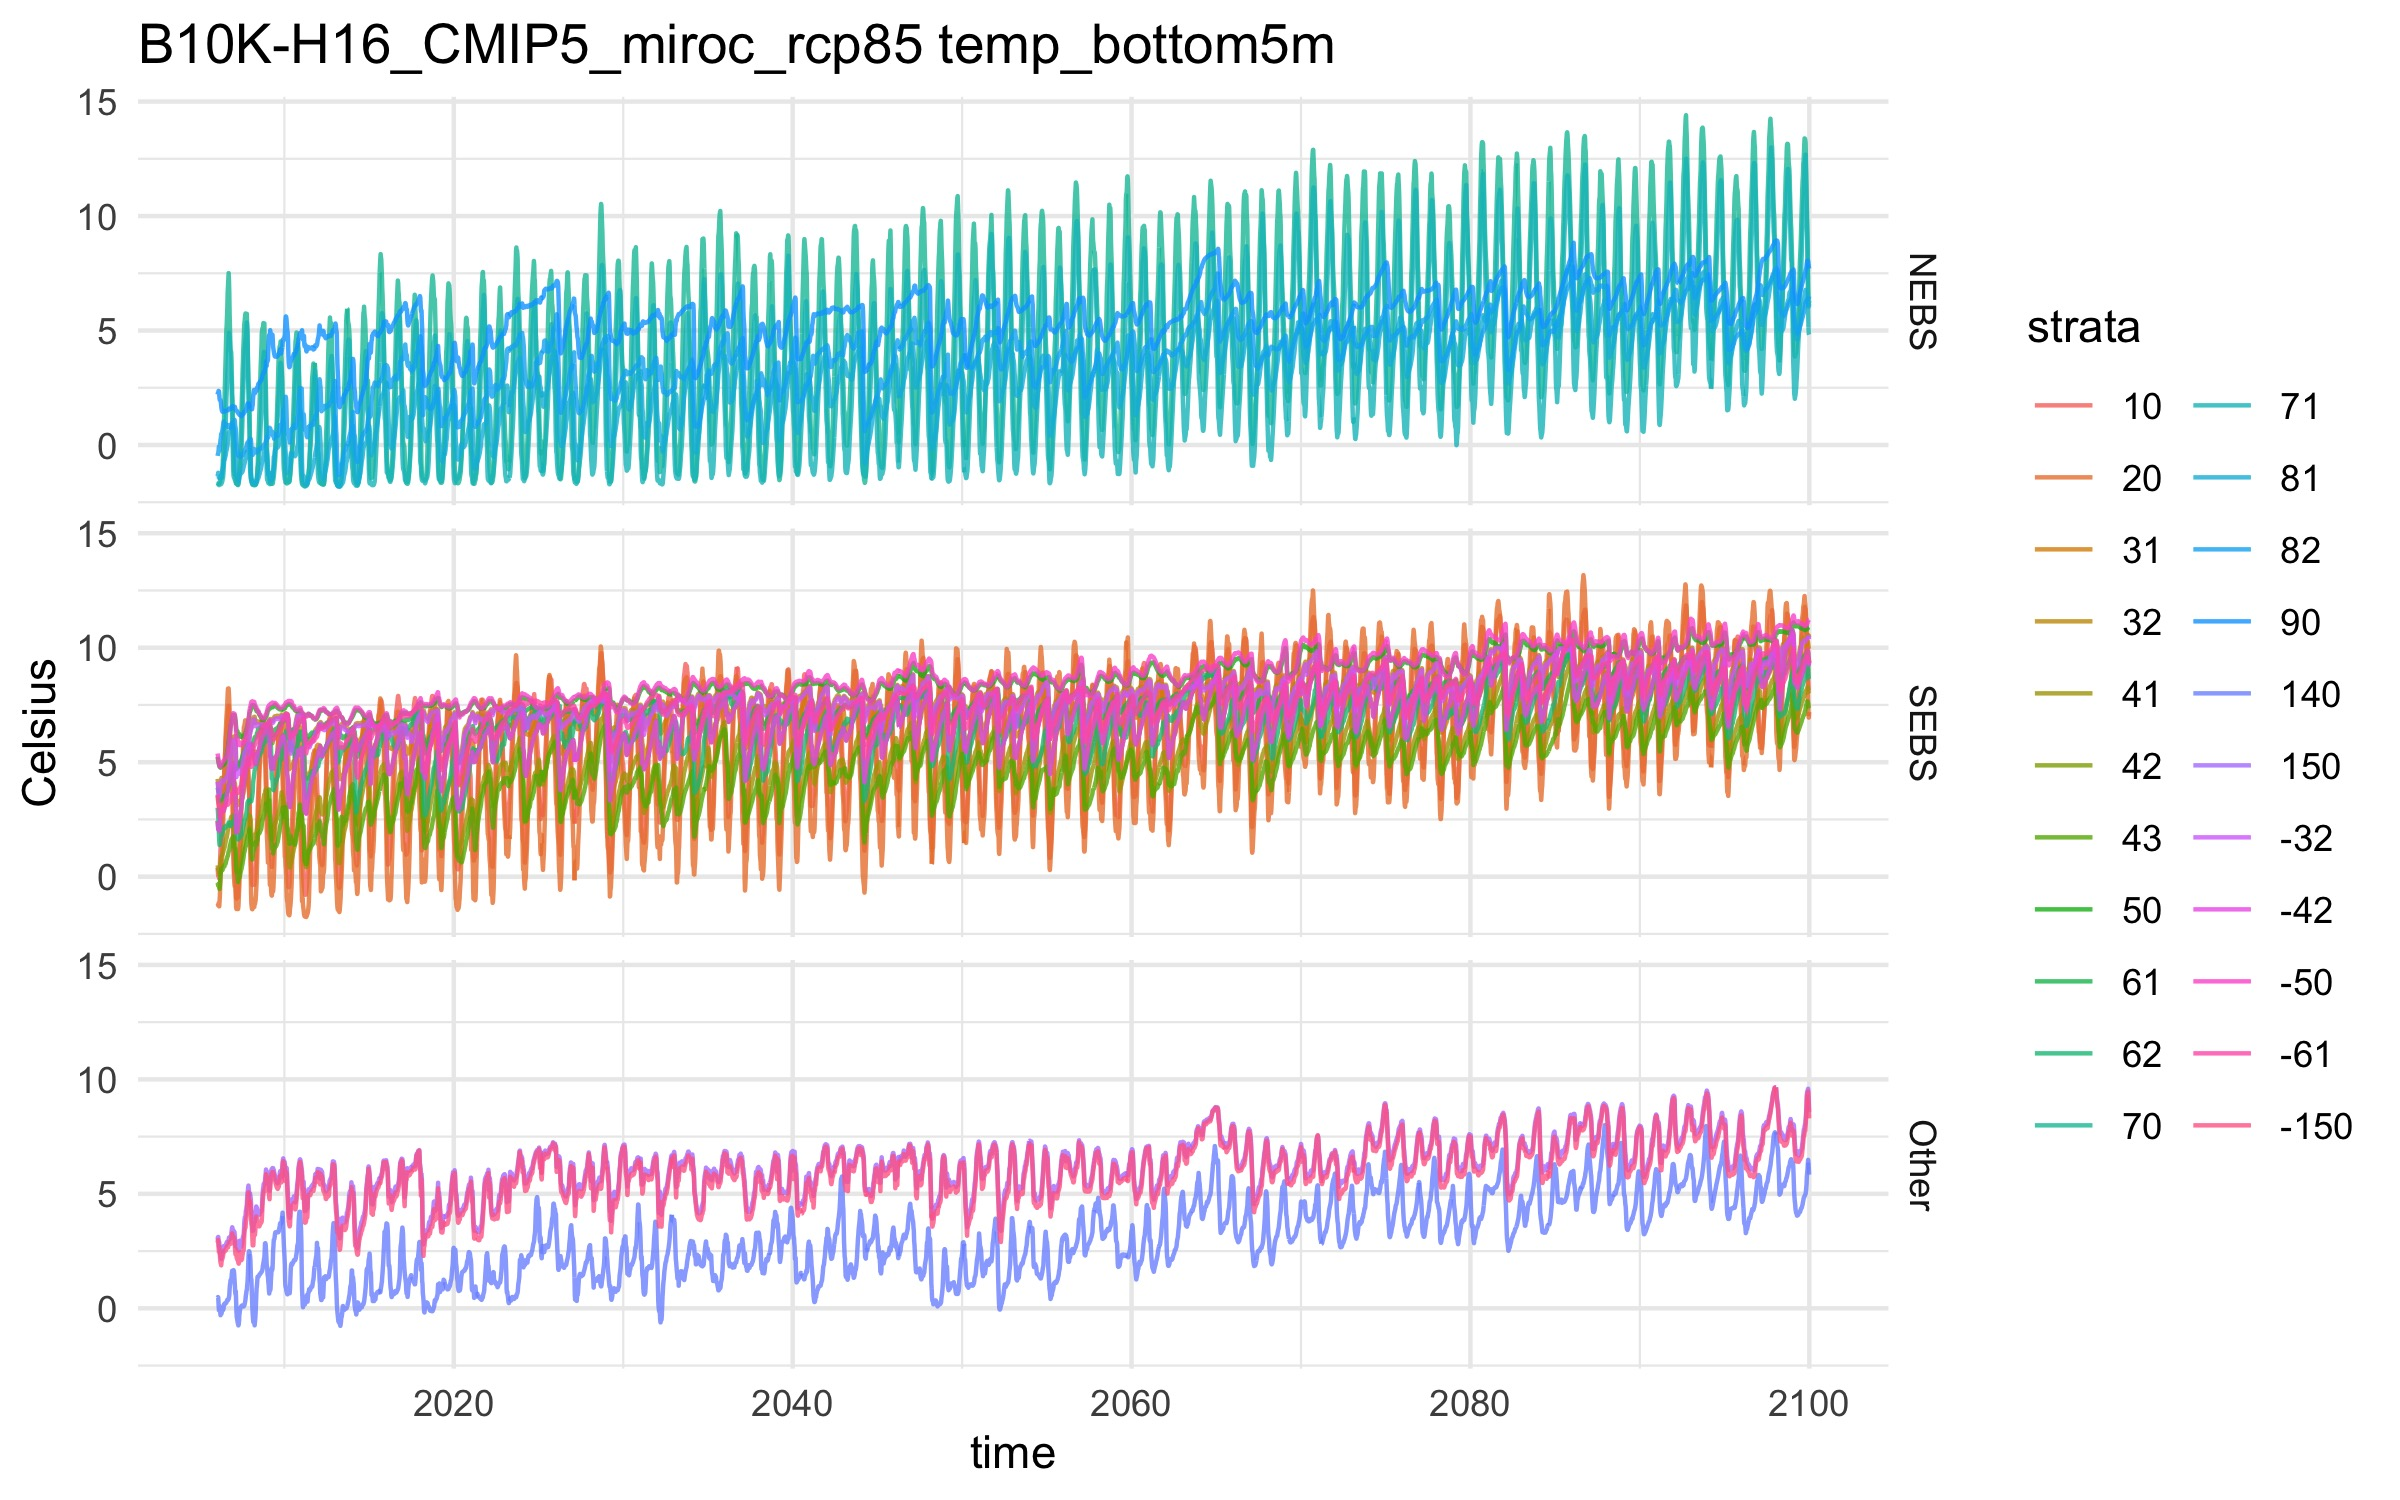
\includegraphics[width=0.65\textwidth,height=\textheight]{Figs/weekly_bystrata.jpg}
\caption{Weekly indcices by sub-region}
\end{figure}

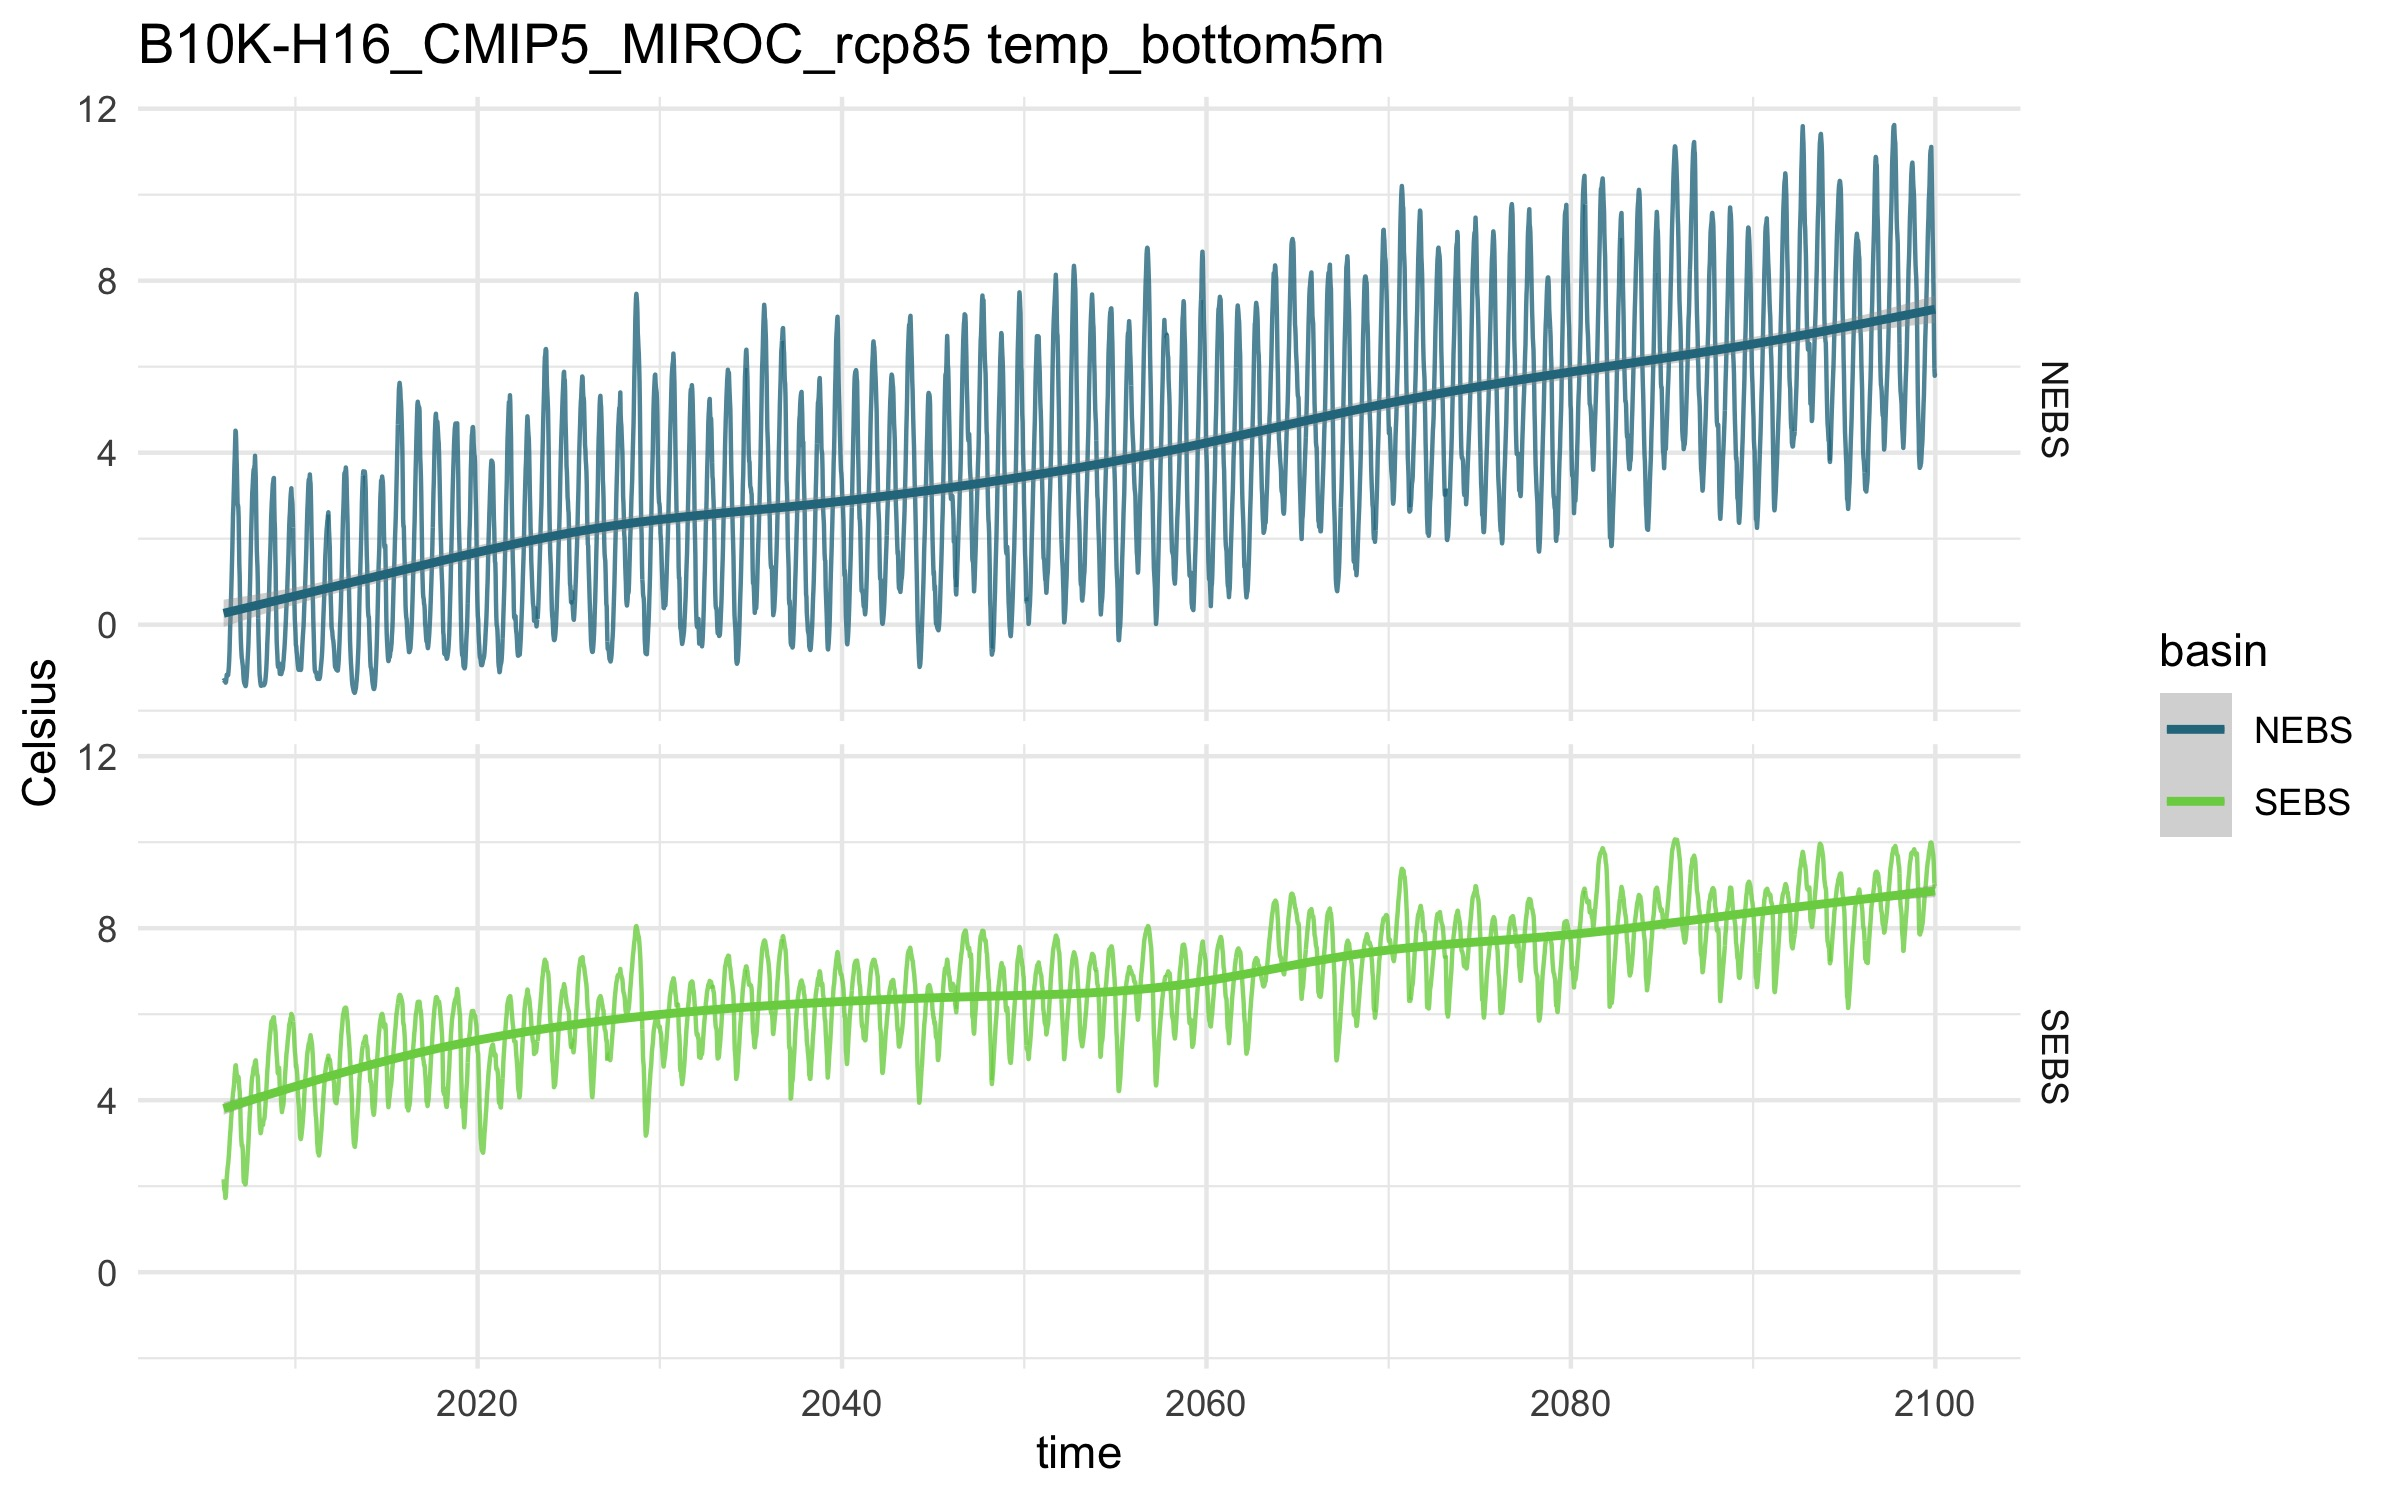
\includegraphics[width=0.65\textwidth,height=\textheight]{Figs/weekly_byreg.jpg}
\#\#\# 6.1.3. Level 3 projections: Seasonal averages

Now using a similar approach get the monthly mean values for a variable:

\begin{Shaded}
\begin{Highlighting}[]
\NormalTok{     sim <-}\StringTok{"B10K-H16_CMIP5_MIROC_rcp85"} 

    \CommentTok{# Set up seasons (this follows Holsman et al. 2020)}
\NormalTok{      seasons <-}\StringTok{ }\KeywordTok{data.frame}\NormalTok{(}\DataTypeTok{mo =} \DecValTok{1}\OperatorTok{:}\DecValTok{12}\NormalTok{, }
                   \DataTypeTok{season =}\KeywordTok{factor}\NormalTok{(}\StringTok{""}\NormalTok{,}
                     \DataTypeTok{levels=}\KeywordTok{c}\NormalTok{(}\StringTok{"Winter"}\NormalTok{,}\StringTok{"Spring"}\NormalTok{,}\StringTok{"Summer"}\NormalTok{,}\StringTok{"Fall"}\NormalTok{)))}
\NormalTok{      seasons}\OperatorTok{$}\NormalTok{season[}\DecValTok{1}\OperatorTok{:}\DecValTok{3}\NormalTok{]   <-}\StringTok{ "Winter"}
\NormalTok{      seasons}\OperatorTok{$}\NormalTok{season[}\DecValTok{4}\OperatorTok{:}\DecValTok{6}\NormalTok{]   <-}\StringTok{ "Spring"}
\NormalTok{      seasons}\OperatorTok{$}\NormalTok{season[}\DecValTok{7}\OperatorTok{:}\DecValTok{9}\NormalTok{]   <-}\StringTok{ "Summer"}
\NormalTok{      seasons}\OperatorTok{$}\NormalTok{season[}\DecValTok{10}\OperatorTok{:}\DecValTok{12}\NormalTok{] <-}\StringTok{ "Fall"}
    
       
\NormalTok{    vl <-}\StringTok{ }\KeywordTok{c}\NormalTok{(}
                  \StringTok{"temp_bottom5m"}\NormalTok{,}
                  \StringTok{"NCaS_integrated"}\NormalTok{, }\CommentTok{# Large Cop}
                  \StringTok{"Cop_integrated"}\NormalTok{,  }\CommentTok{# Small Cop}
                  \StringTok{"EupS_integrated"}\NormalTok{) }\CommentTok{# Euphausiids}
    
    \CommentTok{# create local rdata files (opt 1)}
    \ControlFlowTok{if}\NormalTok{(}\OperatorTok{!}\KeywordTok{file.exists}\NormalTok{(}\KeywordTok{file.path}\NormalTok{(Rdata_path,fl)))}
      \KeywordTok{get_l3}\NormalTok{(}\DataTypeTok{web_nc =} \OtherTok{TRUE}\NormalTok{, }\DataTypeTok{download_nc =}\NormalTok{ F,}
          \DataTypeTok{varlist =}\NormalTok{ vl,}\DataTypeTok{sim_list =}\NormalTok{ sim)}
    
    \CommentTok{# open a "region" or strata specific  file}
\NormalTok{    fl      <-}\StringTok{ }\KeywordTok{file.path}\NormalTok{(sim,}\KeywordTok{paste0}\NormalTok{(reg_txt,sim,}\StringTok{".Rdata"}\NormalTok{))}
    \KeywordTok{load}\NormalTok{(}\KeywordTok{file.path}\NormalTok{(main,Rdata_path,fl))}
    
    \CommentTok{# get large zooplankton as the sum of euph and NCaS}
\NormalTok{    tmp_var    <-}\StringTok{ }\NormalTok{ACLIMregion}\OperatorTok
\StringTok{      }\KeywordTok{filter}\NormalTok{(var}\OperatorTok\NormalTok{vl[}\KeywordTok{c}\NormalTok{(}\DecValTok{2}\NormalTok{,}\DecValTok{3}\NormalTok{)])}\OperatorTok
\StringTok{      }\KeywordTok{group_by}\NormalTok{(time,strata,strata_area_km2,basin)}\OperatorTok
\StringTok{      }\KeywordTok{group_by}\NormalTok{(time,}
\NormalTok{             strata,}
\NormalTok{             strata_area_km2,}
\NormalTok{             basin,}
\NormalTok{             units)}\OperatorTok
\StringTok{      }\KeywordTok{summarise}\NormalTok{(}\DataTypeTok{val =}\KeywordTok{sum}\NormalTok{(val))}\OperatorTok
\StringTok{      }\KeywordTok{mutate}\NormalTok{(}\DataTypeTok{var       =} \StringTok{"Zoop_integrated"}\NormalTok{,}
             \DataTypeTok{long_name =}\StringTok{"Total On-shelf }
\StringTok{             large zooplankton concentration, }
\StringTok{             integrated over depth (NCa, Eup)"}\NormalTok{)}
    
    \KeywordTok{rm}\NormalTok{(ACLIMregion)}
    \KeywordTok{head}\NormalTok{(tmp_var)}
    
\NormalTok{    tmp_var}\OperatorTok{$}\NormalTok{yr     <-}\StringTok{ }\KeywordTok{strptime}\NormalTok{(}\KeywordTok{as.Date}\NormalTok{(tmp_var}\OperatorTok{$}\NormalTok{time),}
                               \DataTypeTok{format=}\StringTok{"%Y-%m-%d"}\NormalTok{)}\OperatorTok{$}\NormalTok{year }\OperatorTok{+}\StringTok{ }\DecValTok{1900}
\NormalTok{    tmp_var}\OperatorTok{$}\NormalTok{mo     <-}\StringTok{ }\KeywordTok{strptime}\NormalTok{(}\KeywordTok{as.Date}\NormalTok{(tmp_var}\OperatorTok{$}\NormalTok{time),}
                               \DataTypeTok{format=}\StringTok{"%Y-%m-%d"}\NormalTok{)}\OperatorTok{$}\NormalTok{mon  }\OperatorTok{+}\StringTok{ }\DecValTok{1}
\NormalTok{    tmp_var}\OperatorTok{$}\NormalTok{jday   <-}\StringTok{ }\KeywordTok{strptime}\NormalTok{(}\KeywordTok{as.Date}\NormalTok{(tmp_var}\OperatorTok{$}\NormalTok{time),}
                               \DataTypeTok{format=}\StringTok{"%Y-%m-%d"}\NormalTok{)}\OperatorTok{$}\NormalTok{yday }\OperatorTok{+}\StringTok{ }\DecValTok{1}
\NormalTok{    tmp_var}\OperatorTok{$}\NormalTok{season <-}\StringTok{ }\NormalTok{seasons[tmp_var}\OperatorTok{$}\NormalTok{mo,}\DecValTok{2}\NormalTok{]}
    
    \CommentTok{# To get the average value for a set of strata, weight the val by the area: (slow...)}
\NormalTok{    mn_NEBS_season <-}\StringTok{ }\KeywordTok{getAVGnSUM}\NormalTok{(}
      \DataTypeTok{strataIN =}\NormalTok{ NEBS_strata,}
      \DataTypeTok{dataIN =}\NormalTok{ tmp_var,}
      \DataTypeTok{tblock=}\KeywordTok{c}\NormalTok{(}\StringTok{"yr"}\NormalTok{,}\StringTok{"season"}\NormalTok{))}
\NormalTok{    mn_NEBS_season}\OperatorTok{$}\NormalTok{basin =}\StringTok{ "NEBS"}
\NormalTok{    mn_SEBS_season <-}\StringTok{ }\KeywordTok{getAVGnSUM}\NormalTok{(}
      \DataTypeTok{strataIN =}\NormalTok{ SEBS_strata, }
      \DataTypeTok{dataIN =}\NormalTok{ tmp_var,}
      \DataTypeTok{tblock=}\KeywordTok{c}\NormalTok{(}\StringTok{"yr"}\NormalTok{,}\StringTok{"season"}\NormalTok{))}
\NormalTok{    mn_SEBS_season}\OperatorTok{$}\NormalTok{basin =}\StringTok{ "SEBS"}
    
\NormalTok{   plot_data      <-}\StringTok{ }\KeywordTok{rbind}\NormalTok{(mn_NEBS_season,mn_SEBS_season)}
    
   \CommentTok{# plot Fall values:}
\NormalTok{   p6 <-}\StringTok{ }\KeywordTok{ggplot}\NormalTok{(}\DataTypeTok{data =}\NormalTok{ plot_data}\OperatorTok\KeywordTok{filter}\NormalTok{(season}\OperatorTok{==}\StringTok{"Fall"}\NormalTok{) ) }\OperatorTok{+}\StringTok{ }
\StringTok{      }\KeywordTok{geom_line}\NormalTok{(   }\KeywordTok{aes}\NormalTok{(}\DataTypeTok{x =}\NormalTok{ yr,}\DataTypeTok{y =}\NormalTok{ mn_val,}\DataTypeTok{color=}\NormalTok{basin),}\DataTypeTok{alpha=}\NormalTok{.}\DecValTok{8}\NormalTok{)}\OperatorTok{+}
\StringTok{      }\KeywordTok{geom_smooth}\NormalTok{( }\KeywordTok{aes}\NormalTok{(}\DataTypeTok{x =}\NormalTok{ yr,}\DataTypeTok{y =}\NormalTok{ mn_val,}\DataTypeTok{color=}\NormalTok{basin),}
                  \DataTypeTok{formula =}\NormalTok{ y }\OperatorTok{~}\StringTok{ }\NormalTok{x, }\DataTypeTok{se =}\NormalTok{ T)}\OperatorTok{+}
\StringTok{      }\KeywordTok{facet_grid}\NormalTok{(basin}\OperatorTok{~}\NormalTok{.)}\OperatorTok{+}
\StringTok{      }\KeywordTok{scale_color_viridis_d}\NormalTok{(}\DataTypeTok{begin=}\NormalTok{.}\DecValTok{4}\NormalTok{,}\DataTypeTok{end=}\NormalTok{.}\DecValTok{8}\NormalTok{)}\OperatorTok{+}
\StringTok{      }\KeywordTok{ylab}\NormalTok{(tmp_var}\OperatorTok{$}\NormalTok{units[}\DecValTok{1}\NormalTok{])}\OperatorTok{+}
\StringTok{      }\KeywordTok{ggtitle}\NormalTok{( }\KeywordTok{paste}\NormalTok{(sim,}\StringTok{"Fall"}\NormalTok{,mn_NEBS_season}\OperatorTok{$}\NormalTok{var[}\DecValTok{1}\NormalTok{]))}\OperatorTok{+}
\StringTok{      }\KeywordTok{theme_minimal}\NormalTok{()}
\NormalTok{  p6}
  
  
  \ControlFlowTok{if}\NormalTok{(update.figs)  }
    \KeywordTok{ggsave}\NormalTok{(}\DataTypeTok{file=}\KeywordTok{file.path}\NormalTok{(main,}\StringTok{"Figs/Fall_large_Zoop.jpg"}\NormalTok{),}\DataTypeTok{width=}\DecValTok{8}\NormalTok{,}\DataTypeTok{height=}\DecValTok{5}\NormalTok{)}
\end{Highlighting}
\end{Shaded}

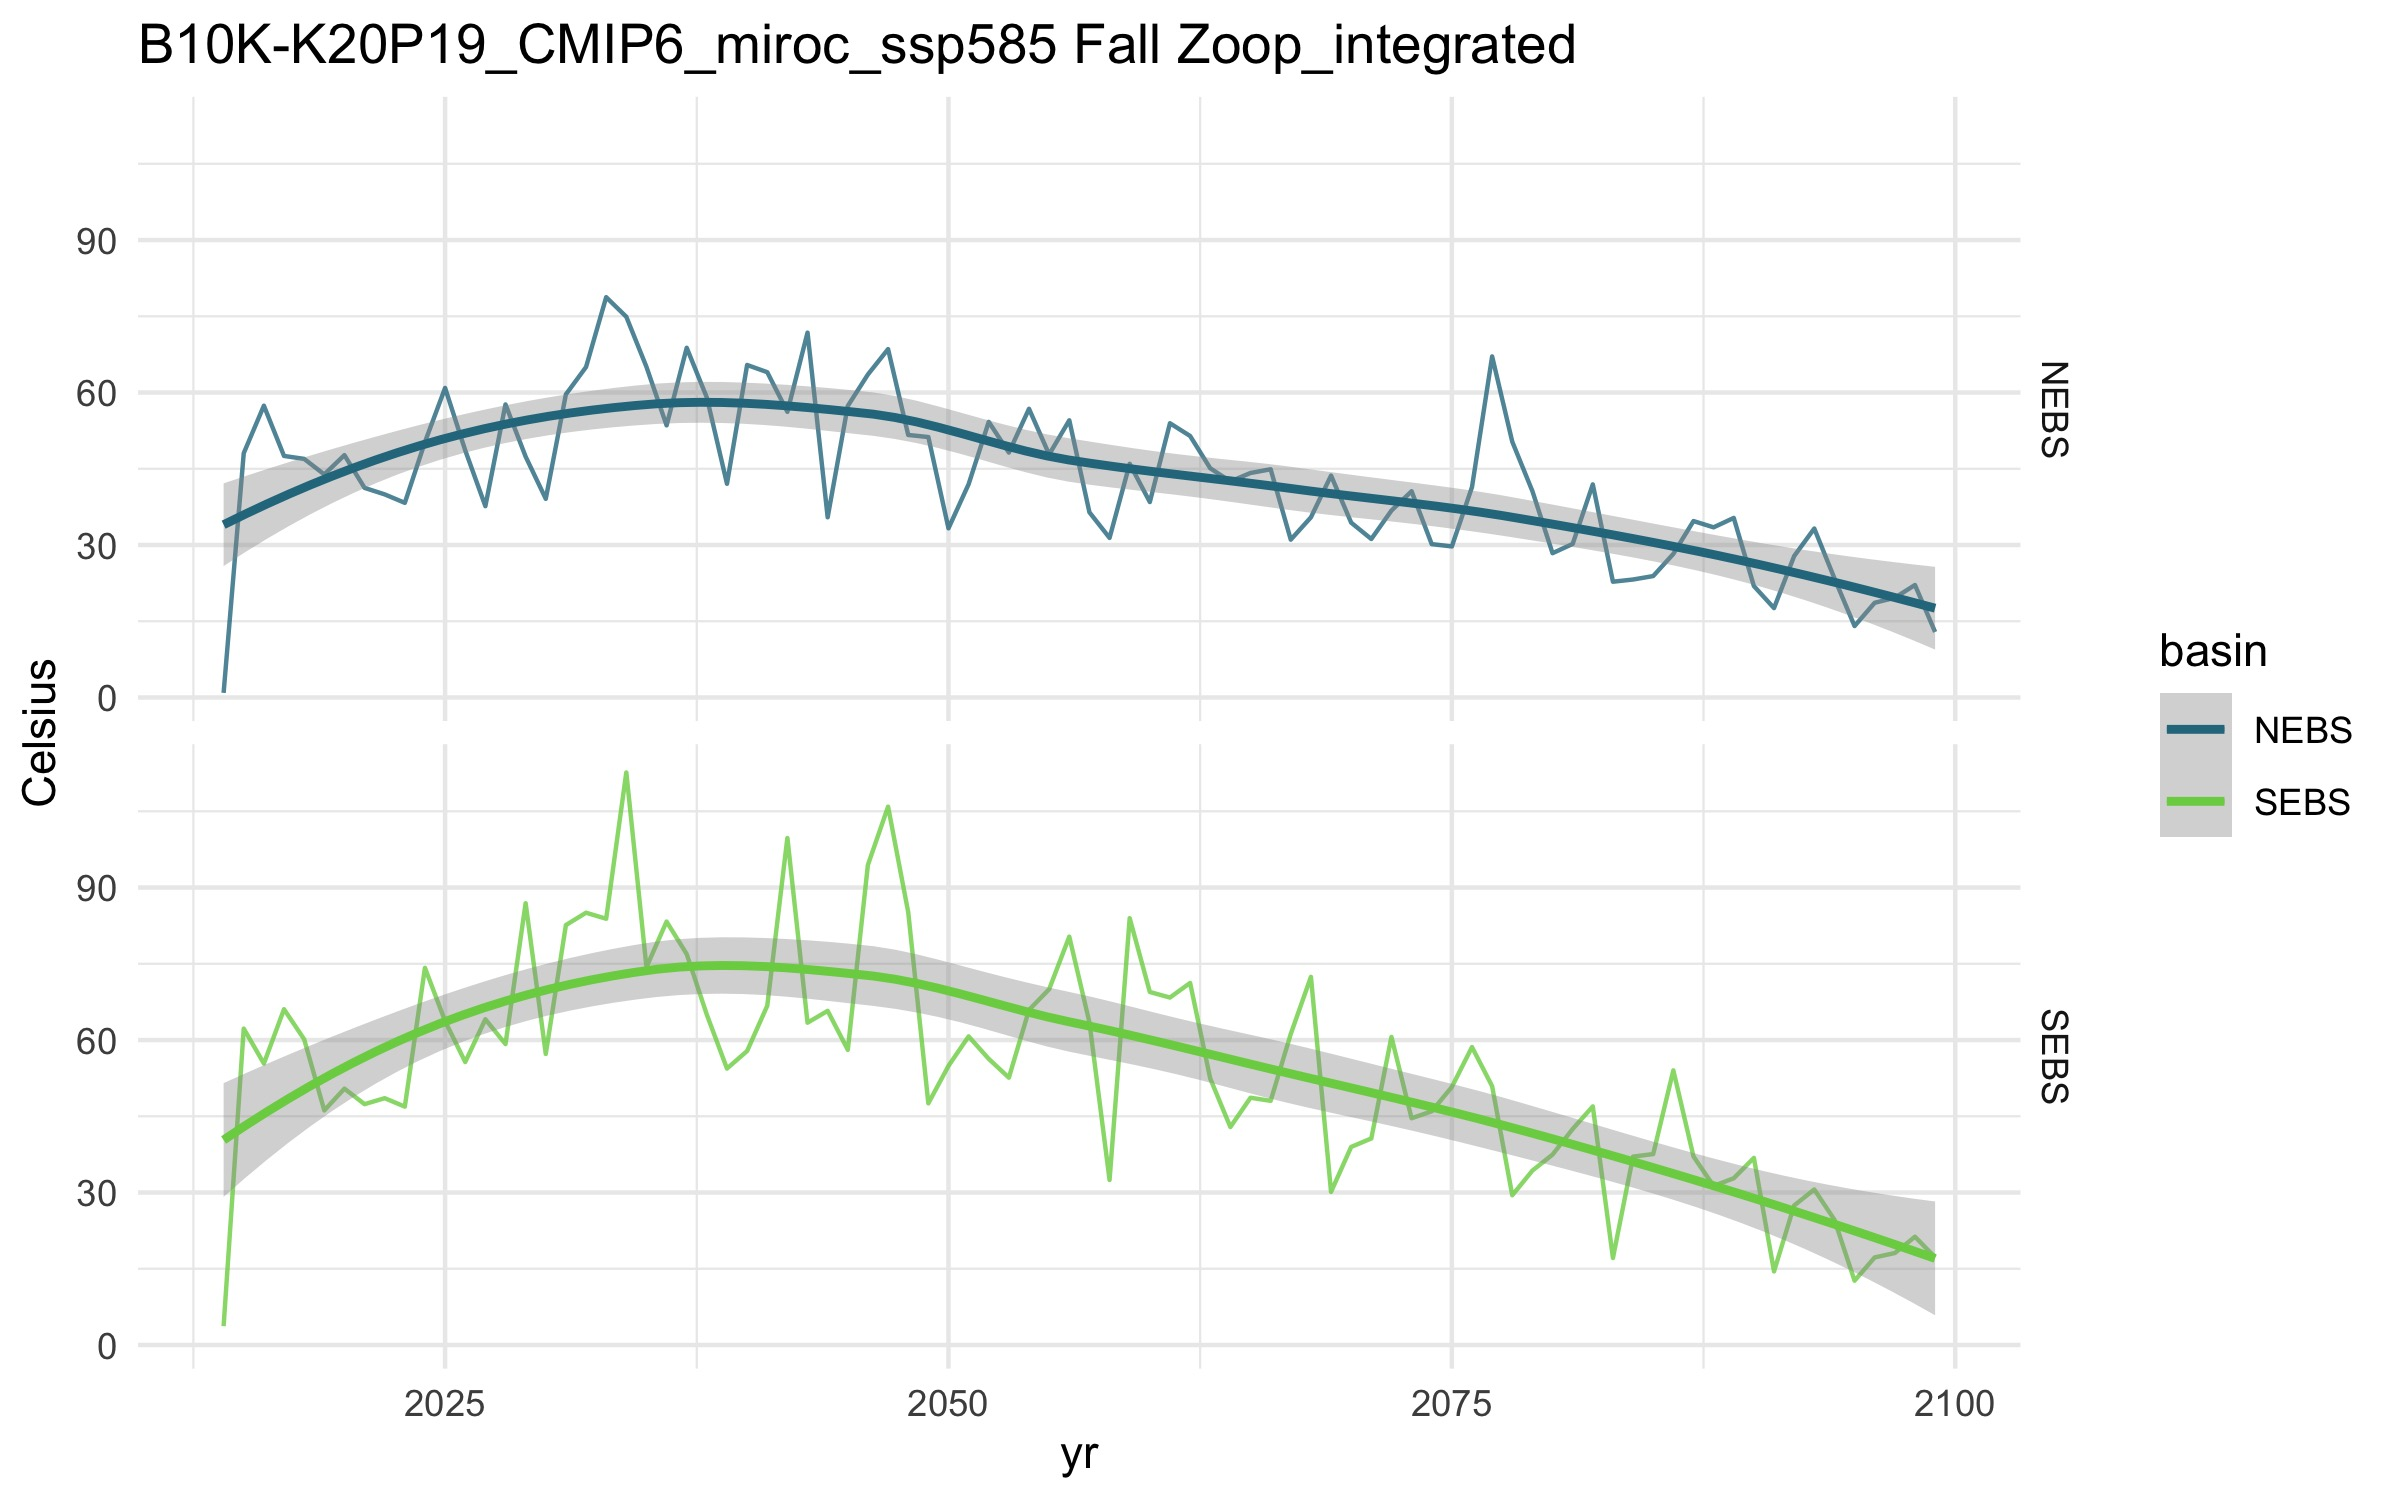
\includegraphics[width=0.65\textwidth,height=\textheight]{Figs/Fall_large_Zoop.jpg}
\#\#\# 6.1.4. Level 3 Projections: Monthly averages Using the same
approach we can get monthly averages for a given variable:

\begin{Shaded}
\begin{Highlighting}[]
    \CommentTok{# To get the average value for a set of strata, weight the val by the area: (slow...)}
\NormalTok{    mn_NEBS_season <-}\StringTok{ }\KeywordTok{getAVGnSUM}\NormalTok{(}
      \DataTypeTok{strataIN =}\NormalTok{ NEBS_strata,}
      \DataTypeTok{dataIN   =}\NormalTok{ tmp_var,}
      \DataTypeTok{tblock   =} \KeywordTok{c}\NormalTok{(}\StringTok{"yr"}\NormalTok{,}\StringTok{"mo"}\NormalTok{))}
\NormalTok{    mn_NEBS_season}\OperatorTok{$}\NormalTok{basin =}\StringTok{ "NEBS"}
\NormalTok{    mn_SEBS_season <-}\StringTok{ }\KeywordTok{getAVGnSUM}\NormalTok{(}
      \DataTypeTok{strataIN =}\NormalTok{ SEBS_strata, }
      \DataTypeTok{dataIN =}\NormalTok{ tmp_var,}
      \DataTypeTok{tblock=}\KeywordTok{c}\NormalTok{(}\StringTok{"yr"}\NormalTok{,}\StringTok{"mo"}\NormalTok{))}
\NormalTok{    mn_SEBS_season}\OperatorTok{$}\NormalTok{basin =}\StringTok{ "SEBS"}
    
\NormalTok{    plot_data      <-}\StringTok{ }\KeywordTok{rbind}\NormalTok{(mn_NEBS_season,mn_SEBS_season)}
    
   \CommentTok{# plot Fall values:}
\NormalTok{   p7 <-}\StringTok{ }\KeywordTok{ggplot}\NormalTok{(}\DataTypeTok{data =}\NormalTok{ plot_data}\OperatorTok\KeywordTok{filter}\NormalTok{(mo}\OperatorTok{==}\DecValTok{9}\NormalTok{) ) }\OperatorTok{+}\StringTok{ }
\StringTok{      }\KeywordTok{geom_line}\NormalTok{(   }\KeywordTok{aes}\NormalTok{(}\DataTypeTok{x =}\NormalTok{ yr,}\DataTypeTok{y =}\NormalTok{ mn_val,}\DataTypeTok{color=}\NormalTok{basin),}\DataTypeTok{alpha=}\NormalTok{.}\DecValTok{8}\NormalTok{)}\OperatorTok{+}
\StringTok{      }\KeywordTok{geom_smooth}\NormalTok{( }\KeywordTok{aes}\NormalTok{(}\DataTypeTok{x =}\NormalTok{ yr,}\DataTypeTok{y =}\NormalTok{ mn_val,}\DataTypeTok{color=}\NormalTok{basin),}
                  \DataTypeTok{formula =}\NormalTok{ y }\OperatorTok{~}\StringTok{ }\NormalTok{x, }\DataTypeTok{se =}\NormalTok{ T)}\OperatorTok{+}
\StringTok{      }\KeywordTok{facet_grid}\NormalTok{(basin}\OperatorTok{~}\NormalTok{.)}\OperatorTok{+}
\StringTok{      }\KeywordTok{scale_color_viridis_d}\NormalTok{(}\DataTypeTok{begin=}\NormalTok{.}\DecValTok{4}\NormalTok{,}\DataTypeTok{end=}\NormalTok{.}\DecValTok{8}\NormalTok{)}\OperatorTok{+}
\StringTok{      }\KeywordTok{ylab}\NormalTok{(tmp_var}\OperatorTok{$}\NormalTok{units[}\DecValTok{1}\NormalTok{])}\OperatorTok{+}
\StringTok{      }\KeywordTok{ggtitle}\NormalTok{( }\KeywordTok{paste}\NormalTok{(aclim[}\DecValTok{2}\NormalTok{],}\StringTok{"Sept."}\NormalTok{,mn_NEBS_season}\OperatorTok{$}\NormalTok{var[}\DecValTok{1}\NormalTok{]))}\OperatorTok{+}
\StringTok{      }\KeywordTok{theme_minimal}\NormalTok{()}
\NormalTok{  p7}
  
  \ControlFlowTok{if}\NormalTok{(update.figs)  }
    \KeywordTok{ggsave}\NormalTok{(}\DataTypeTok{file=}\KeywordTok{file.path}\NormalTok{(main,}\StringTok{"Figs/Sept_large_Zoop.jpg"}\NormalTok{),}\DataTypeTok{width=}\DecValTok{8}\NormalTok{,}\DataTypeTok{height=}\DecValTok{5}\NormalTok{)}
\end{Highlighting}
\end{Shaded}

\begin{figure}
\centering
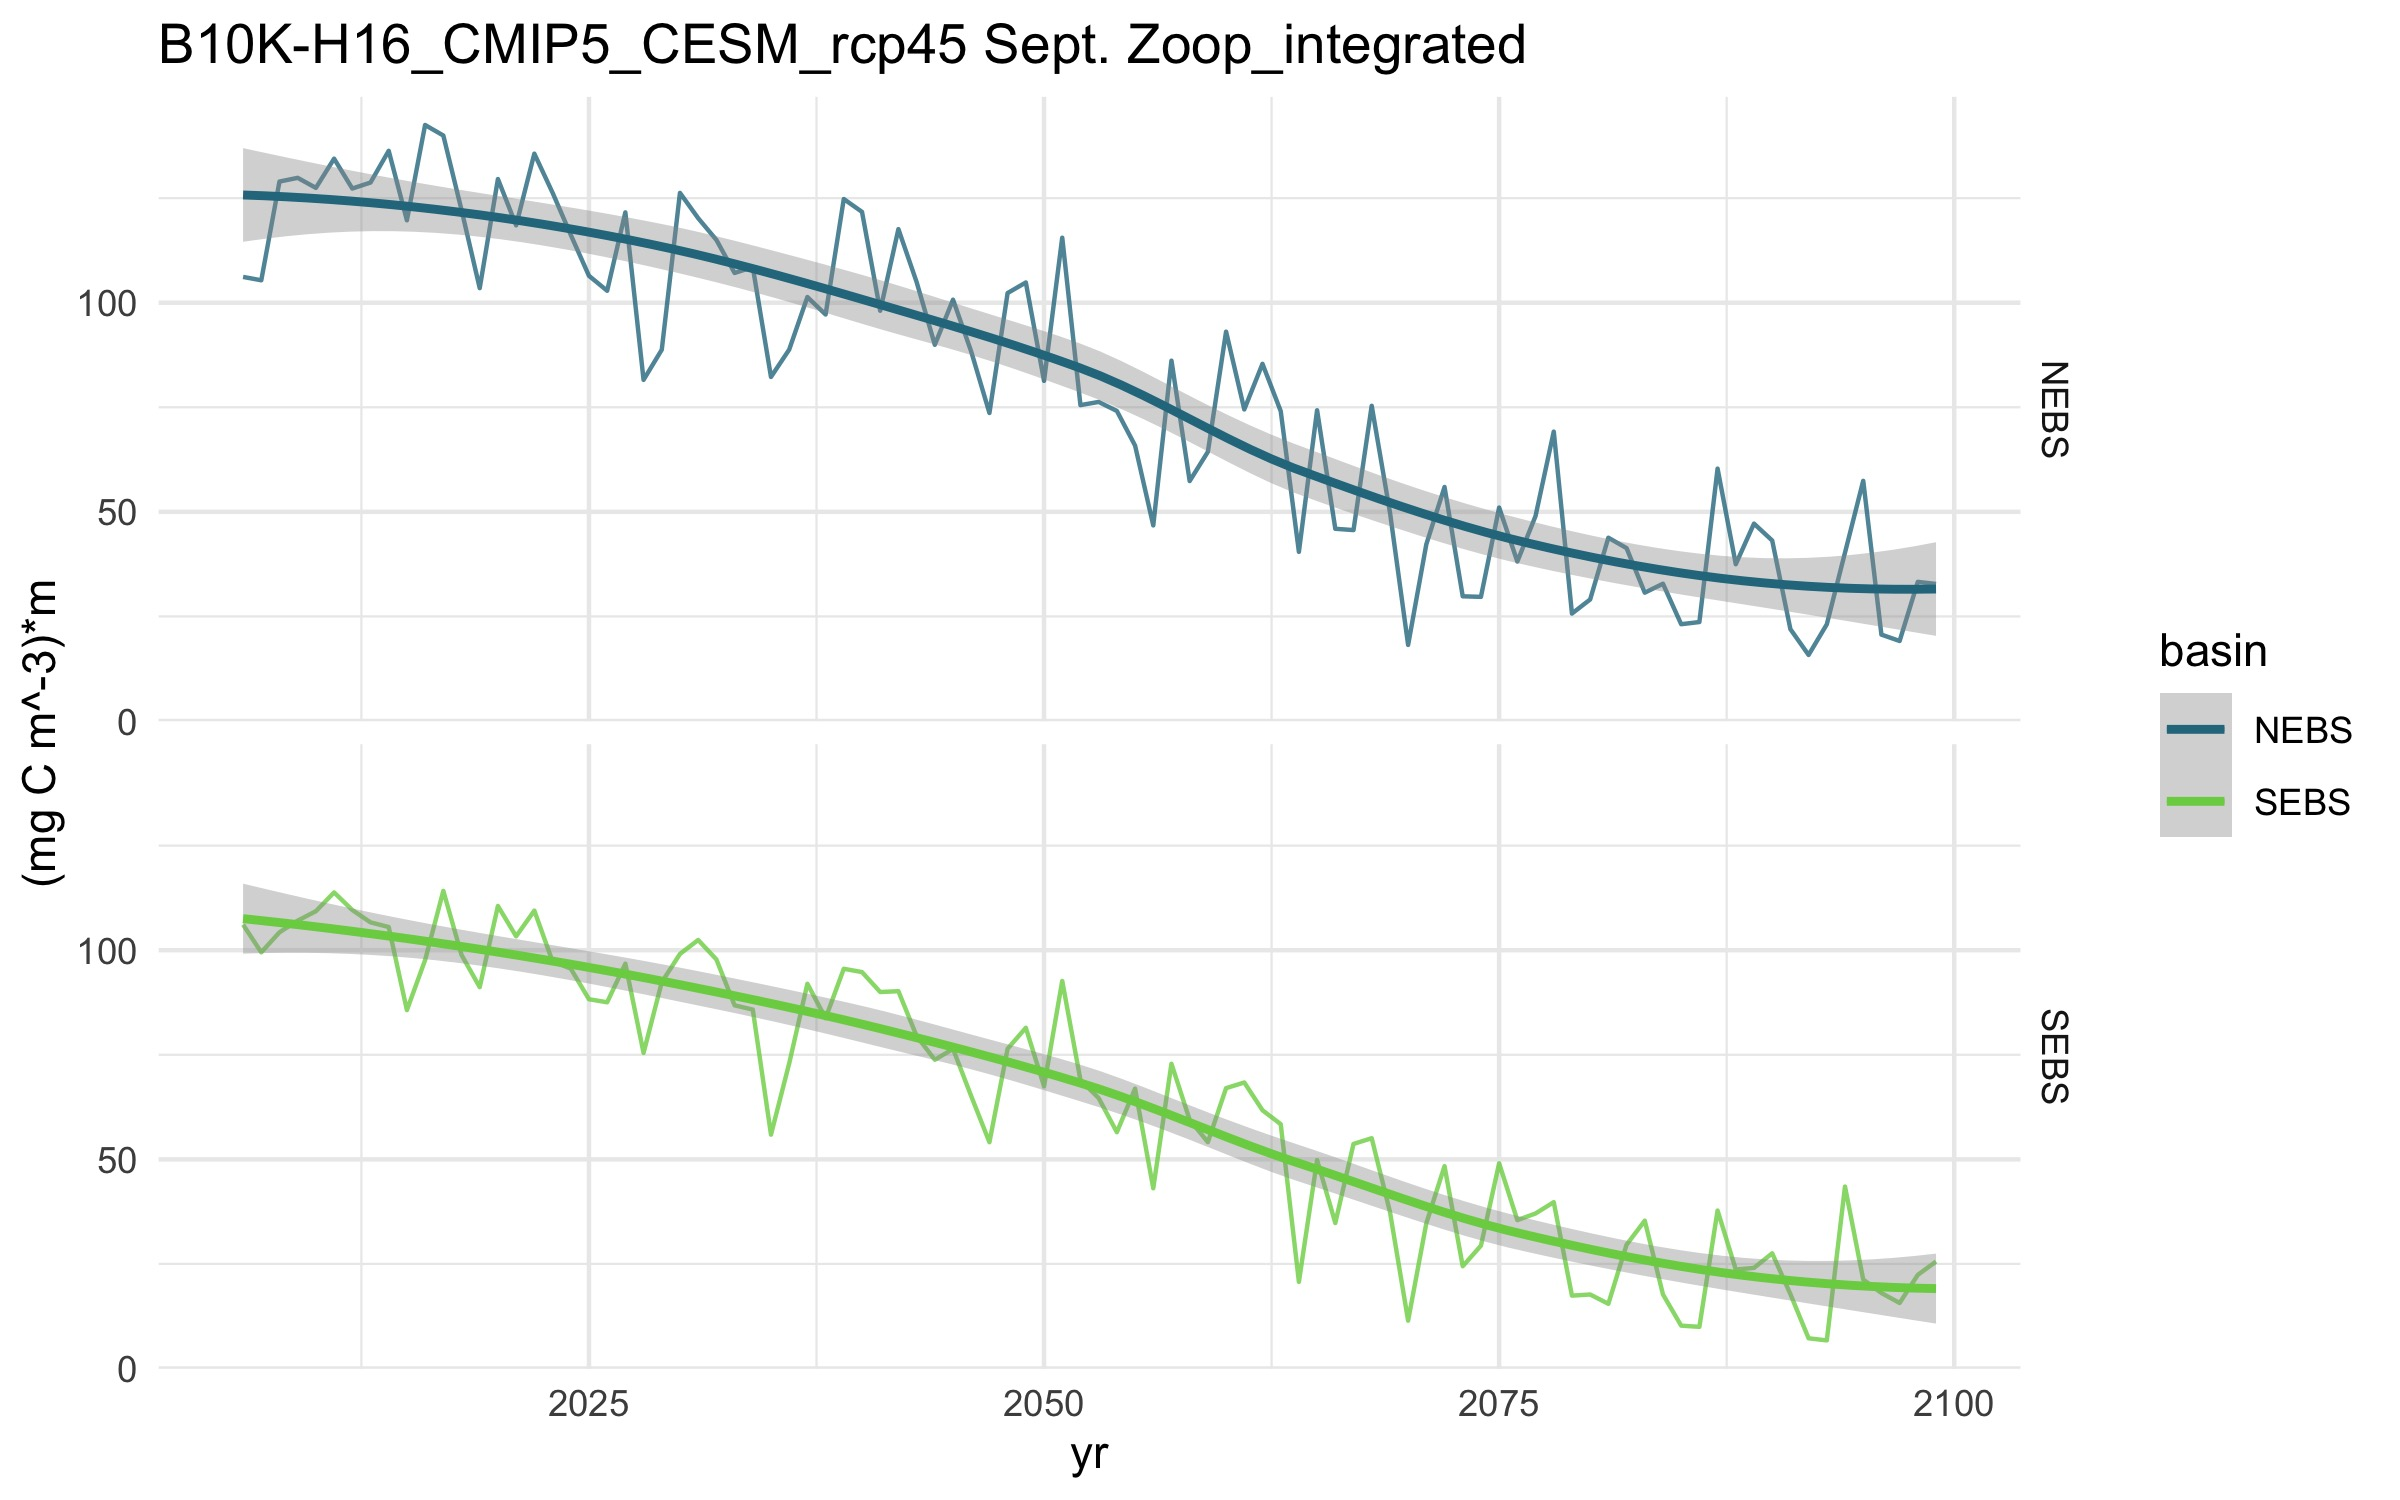
\includegraphics[width=0.65\textwidth,height=\textheight]{Figs/Sept_large_Zoop.jpg}
\caption{September large zooplankton integrated concentration}
\end{figure}

Finally we can use this approach to plot the monthly averages and look
for phenological shifts:

\begin{Shaded}
\begin{Highlighting}[]
  \CommentTok{# or average in 4 time slices by mo:}
  \CommentTok{# now create plots of average BT during four time periods}
\NormalTok{    time_seg   <-}\StringTok{ }\KeywordTok{list}\NormalTok{( }\StringTok{'2010-2020'}\NormalTok{ =}\StringTok{ }\KeywordTok{c}\NormalTok{(}\DecValTok{2010}\OperatorTok{:}\DecValTok{2020}\NormalTok{),}
                        \StringTok{'2021-2040'}\NormalTok{ =}\StringTok{ }\KeywordTok{c}\NormalTok{(}\DecValTok{2021}\OperatorTok{:}\DecValTok{2040}\NormalTok{),}
                        \StringTok{'2041-2060'}\NormalTok{ =}\StringTok{ }\KeywordTok{c}\NormalTok{(}\DecValTok{2041}\OperatorTok{:}\DecValTok{2060}\NormalTok{),}
                        \StringTok{'2061-2080'}\NormalTok{ =}\StringTok{ }\KeywordTok{c}\NormalTok{(}\DecValTok{2061}\OperatorTok{:}\DecValTok{2080}\NormalTok{),}
                        \StringTok{'2081-2099'}\NormalTok{ =}\StringTok{ }\KeywordTok{c}\NormalTok{(}\DecValTok{2081}\OperatorTok{:}\DecValTok{2099}\NormalTok{))}
    
\NormalTok{    plot_data}\OperatorTok{$}\NormalTok{ts <-}\KeywordTok{names}\NormalTok{(time_seg)[}\DecValTok{1}\NormalTok{]}
    \ControlFlowTok{for}\NormalTok{(tt }\ControlFlowTok{in} \DecValTok{1}\OperatorTok{:}\KeywordTok{length}\NormalTok{((time_seg)))}
\NormalTok{      plot_data}\OperatorTok{$}\NormalTok{ts[plot_data}\OperatorTok{$}\NormalTok{yr}\OperatorTok\NormalTok{(time_seg[[tt]][}\DecValTok{1}\NormalTok{]}\OperatorTok{:}\NormalTok{time_seg[[tt]][}\DecValTok{2}\NormalTok{])]<-}\KeywordTok{names}\NormalTok{(time_seg)[tt]}
    
\NormalTok{    plot_data2 <-}\StringTok{ }\NormalTok{plot_data}\OperatorTok
\StringTok{      }\KeywordTok{group_by}\NormalTok{(var,mo,units,long_name,basin, ts)}\OperatorTok
\StringTok{      }\KeywordTok{summarize}\NormalTok{(}\DataTypeTok{mn_val2 =} \KeywordTok{mean}\NormalTok{(mn_val))}
   
  \CommentTok{# now plot phenological shift:}
\NormalTok{   p8 <-}\StringTok{ }\KeywordTok{ggplot}\NormalTok{(}\DataTypeTok{data =}\NormalTok{ plot_data2 ) }\OperatorTok{+}\StringTok{ }
\StringTok{      }\KeywordTok{geom_line}\NormalTok{(   }\KeywordTok{aes}\NormalTok{(}\DataTypeTok{x =}\NormalTok{ mo,}\DataTypeTok{y =}\NormalTok{ mn_val2,}\DataTypeTok{color=}\NormalTok{ts),}\DataTypeTok{alpha=}\NormalTok{.}\DecValTok{8}\NormalTok{,}\DataTypeTok{size=}\DecValTok{0}\NormalTok{)}\OperatorTok{+}
\StringTok{      }\KeywordTok{geom_smooth}\NormalTok{( }\KeywordTok{aes}\NormalTok{(}\DataTypeTok{x =}\NormalTok{ mo,}\DataTypeTok{y =}\NormalTok{ mn_val2,}\DataTypeTok{color=}\NormalTok{ts),}
                  \DataTypeTok{formula =}\NormalTok{ y }\OperatorTok{~}\StringTok{ }\NormalTok{x, }\DataTypeTok{se =}\NormalTok{ F)}\OperatorTok{+}
\StringTok{      }\KeywordTok{facet_grid}\NormalTok{(basin}\OperatorTok{~}\NormalTok{.)}\OperatorTok{+}
\StringTok{      }\KeywordTok{scale_color_viridis_d}\NormalTok{(}\DataTypeTok{begin=}\NormalTok{.}\DecValTok{9}\NormalTok{,}\DataTypeTok{end=}\NormalTok{.}\DecValTok{2}\NormalTok{)}\OperatorTok{+}
\StringTok{      }\KeywordTok{ylab}\NormalTok{(tmp_var}\OperatorTok{$}\NormalTok{units[}\DecValTok{1}\NormalTok{])}\OperatorTok{+}
\StringTok{      }\KeywordTok{ggtitle}\NormalTok{( }\KeywordTok{paste}\NormalTok{(aclim[}\DecValTok{2}\NormalTok{],mn_NEBS_season}\OperatorTok{$}\NormalTok{var[}\DecValTok{1}\NormalTok{]))}\OperatorTok{+}
\StringTok{      }\KeywordTok{theme_minimal}\NormalTok{()}
\NormalTok{  p8}
  \ControlFlowTok{if}\NormalTok{(update.figs)  }
    \KeywordTok{ggsave}\NormalTok{(}\DataTypeTok{file=}\KeywordTok{file.path}\NormalTok{(main,}\StringTok{"Figs/PhenShift_large_Zoop.jpg"}\NormalTok{),}\DataTypeTok{width=}\DecValTok{8}\NormalTok{,}\DataTypeTok{height=}\DecValTok{5}\NormalTok{)}
\end{Highlighting}
\end{Shaded}

\begin{figure}
\centering
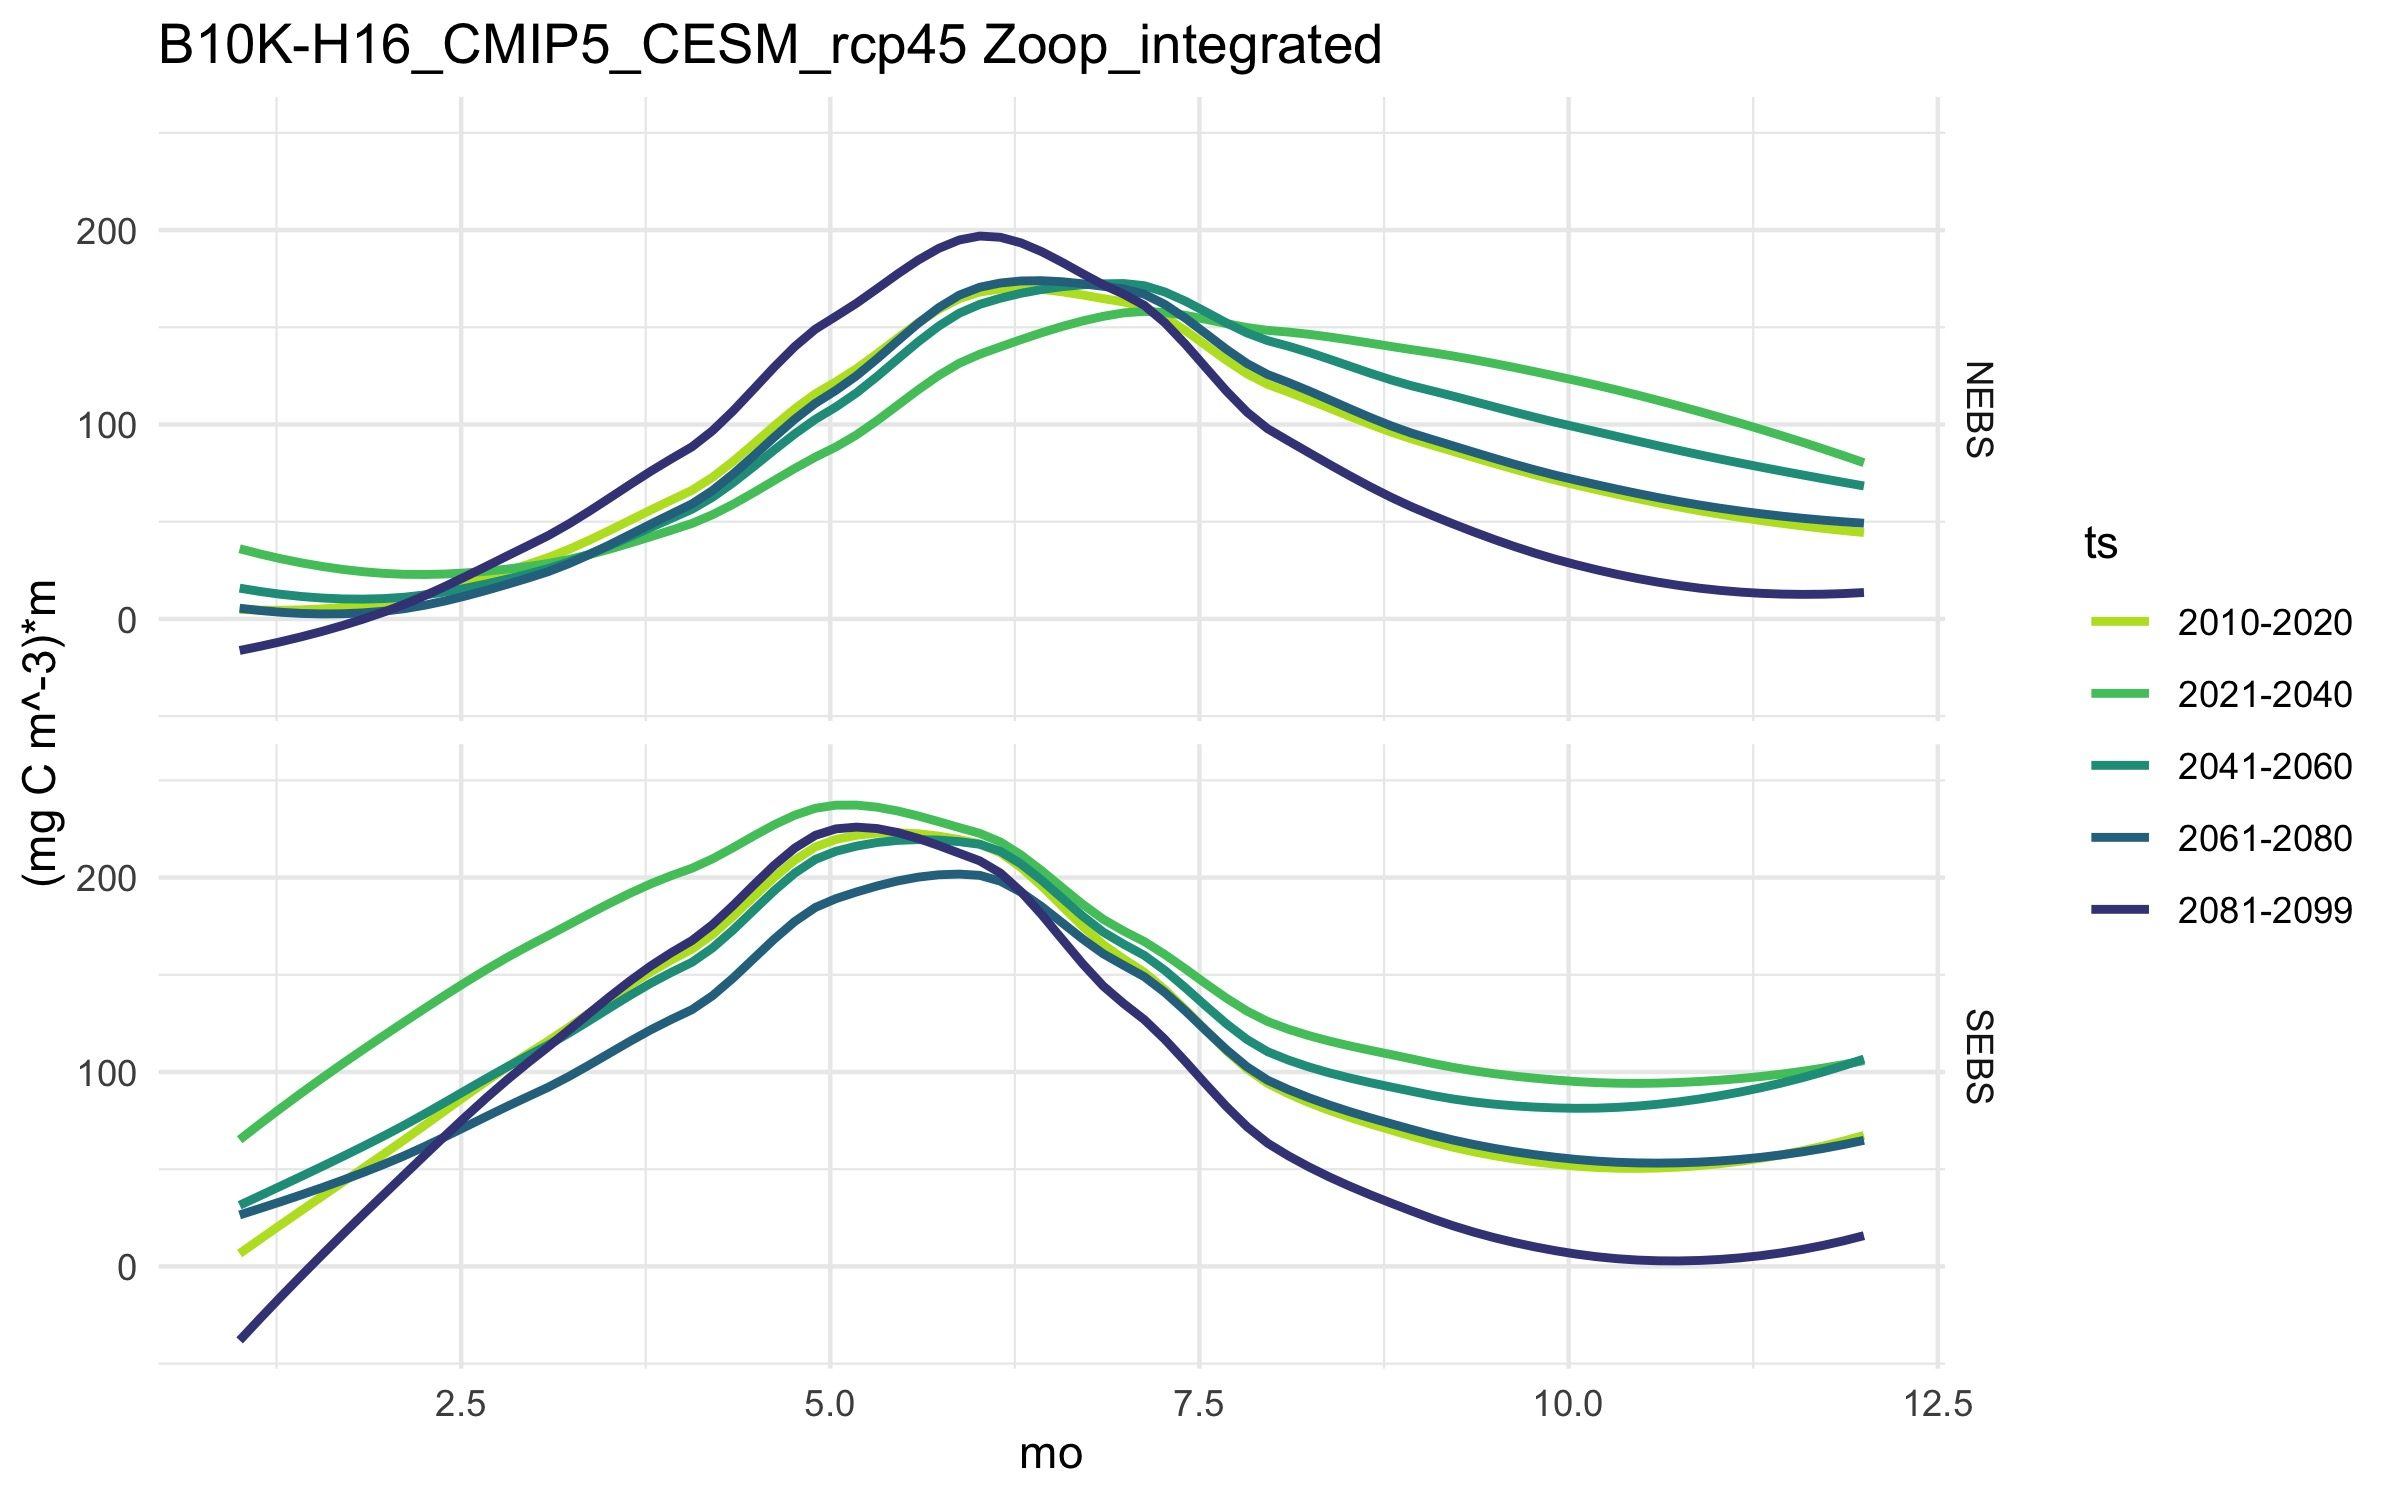
\includegraphics[width=0.65\textwidth,height=\textheight]{Figs/PhenShift_large_Zoop.jpg}
\caption{September large zooplankton integrated concentration}
\end{figure}

\hypertarget{level-2-projections}{%
\subsection{6.2. Level 2 projections}\label{level-2-projections}}

Level 2 data can be explored in the same way as the above indices but we
will focus in the section below on a simple spatial plot and temporal
index. The advantage of Level2 inidces is in the spatial resolution and
values outside of the survey area.

\hypertarget{level-2-projections-custom-spatial-indices}{%
\subsubsection{6.2.1 Level 2 projections: Custom spatial
indices}\label{level-2-projections-custom-spatial-indices}}

\begin{Shaded}
\begin{Highlighting}[]
   \CommentTok{# define four time periods}
\NormalTok{    time_seg   <-}\StringTok{ }\KeywordTok{list}\NormalTok{( }\StringTok{'2010-2020'}\NormalTok{ =}\StringTok{ }\KeywordTok{c}\NormalTok{(}\DecValTok{2000}\OperatorTok{:}\DecValTok{2020}\NormalTok{),}
                        \StringTok{'2021-2040'}\NormalTok{ =}\StringTok{ }\KeywordTok{c}\NormalTok{(}\DecValTok{2021}\OperatorTok{:}\DecValTok{2040}\NormalTok{),}
                        \StringTok{'2041-2060'}\NormalTok{ =}\StringTok{ }\KeywordTok{c}\NormalTok{(}\DecValTok{2041}\OperatorTok{:}\DecValTok{2060}\NormalTok{),}
                        \StringTok{'2061-2080'}\NormalTok{ =}\StringTok{ }\KeywordTok{c}\NormalTok{(}\DecValTok{2061}\OperatorTok{:}\DecValTok{2080}\NormalTok{),}
                        \StringTok{'2081-2099'}\NormalTok{ =}\StringTok{ }\KeywordTok{c}\NormalTok{(}\DecValTok{2081}\OperatorTok{:}\DecValTok{2099}\NormalTok{))}
  
    \CommentTok{# View an individual variable (e.g., Bottom Temp)}
    \CommentTok{# -------------------------------------------------------}
    \KeywordTok{head}\NormalTok{(srvy_vars)}
    \KeywordTok{head}\NormalTok{(aclim)}
    
    \CommentTok{# assign the simulation to download}
    \CommentTok{# --> --> Tinker: try selecting a different set of models to compare}
\NormalTok{    sim        <-}\StringTok{"B10K-H16_CMIP5_MIROC_rcp85"} 
    
\NormalTok{    svl <-}\StringTok{ }\KeywordTok{list}\NormalTok{(}
      \StringTok{'Bottom 5m'}\NormalTok{ =}\StringTok{ "temp"}\NormalTok{,}
      \StringTok{'Surface 5m'}\NormalTok{ =}\StringTok{ "temp"}\NormalTok{,}
      \StringTok{'Integrated'}\NormalTok{ =}\StringTok{ }\KeywordTok{c}\NormalTok{(}\StringTok{"EupS"}\NormalTok{,}\StringTok{"Cop"}\NormalTok{,}\StringTok{"NCaS"}\NormalTok{) ) }
   
    \CommentTok{# Currently available Level 2 variables}
\NormalTok{    dl     <-}\StringTok{ }\NormalTok{proj_l2_datasets}\OperatorTok{$}\NormalTok{dataset  }\CommentTok{# datasets}
   
    
    \CommentTok{# Let's sample the model years as close to Aug 1 as the model timesteps run:}
\NormalTok{    tr          <-}\StringTok{ }\KeywordTok{c}\NormalTok{(}\StringTok{"-08-1 12:00:00 GMT"}\NormalTok{) }
    
    \CommentTok{# the full grid is large and takes a longtime to plot, so let's subsample the grid every 4 cells}
   
\NormalTok{    IDin       <-}\StringTok{ "_Aug1_subgrid"}
\NormalTok{    var_use    <-}\StringTok{ "_bottom5m_temp"}
    
    \CommentTok{# open a "region" or strata specific nc file}
\NormalTok{    fl         <-}\StringTok{ }\KeywordTok{file.path}\NormalTok{(main,Rdata_path,sim,}\StringTok{"Level2"}\NormalTok{,}
                            \KeywordTok{paste0}\NormalTok{(sim,var_use,IDin,}\StringTok{".Rdata"}\NormalTok{))}
    
    \CommentTok{# load object 'ACLIMsurveyrep'}
    \ControlFlowTok{if}\NormalTok{(}\OperatorTok{!}\KeywordTok{file.exists}\NormalTok{(}\KeywordTok{file.path}\NormalTok{(Rdata_path,fl)))}
      \KeywordTok{get_l2}\NormalTok{(}
        \DataTypeTok{ID          =}\NormalTok{ IDin,}
        \DataTypeTok{xi_rangeIN  =} \KeywordTok{seq}\NormalTok{(}\DecValTok{1}\NormalTok{,}\DecValTok{182}\NormalTok{,}\DecValTok{10}\NormalTok{),}
        \DataTypeTok{eta_rangeIN =} \KeywordTok{seq}\NormalTok{(}\DecValTok{1}\NormalTok{,}\DecValTok{258}\NormalTok{,}\DecValTok{10}\NormalTok{),}
        \DataTypeTok{ds_list     =}\NormalTok{ dl,}
        \DataTypeTok{trIN        =}\NormalTok{ tr,}
        \DataTypeTok{sub_varlist =}\NormalTok{ svl,  }
        \DataTypeTok{sim_list    =}\NormalTok{ sim  )}
    
    \CommentTok{# load R data file}
    \KeywordTok{load}\NormalTok{(fl)   }\CommentTok{# temp}
    
    \CommentTok{# there are smarter ways to do this;looping because }
    \CommentTok{# we don't want to mess it up but this is slow...}
\NormalTok{    i <-}\DecValTok{1}
\NormalTok{    data_long <-}\StringTok{ }\KeywordTok{data.frame}\NormalTok{(}\DataTypeTok{latitude =} \KeywordTok{as.vector}\NormalTok{(temp}\OperatorTok{$}\NormalTok{lat),}
                       \DataTypeTok{longitude =} \KeywordTok{as.vector}\NormalTok{(temp}\OperatorTok{$}\NormalTok{lon),}
                       \DataTypeTok{val =} \KeywordTok{as.vector}\NormalTok{(temp}\OperatorTok{$}\NormalTok{val[,,i]),}
                       \DataTypeTok{time =}\NormalTok{ temp}\OperatorTok{$}\NormalTok{time[i],}
                       \DataTypeTok{year =} \KeywordTok{substr}\NormalTok{( temp}\OperatorTok{$}\NormalTok{time[i],}\DecValTok{1}\NormalTok{,}\DecValTok{4}\NormalTok{),}\DataTypeTok{stringsAsFactors =}\NormalTok{ F}
\NormalTok{                       )}
    \ControlFlowTok{for}\NormalTok{(i }\ControlFlowTok{in} \DecValTok{2}\OperatorTok{:}\KeywordTok{dim}\NormalTok{(temp}\OperatorTok{$}\NormalTok{val)[}\DecValTok{3}\NormalTok{])}
\NormalTok{      data_long <-}\StringTok{ }\KeywordTok{rbind}\NormalTok{(data_long,}
                          \KeywordTok{data.frame}\NormalTok{(}\DataTypeTok{latitude =} \KeywordTok{as.vector}\NormalTok{(temp}\OperatorTok{$}\NormalTok{lat),}
                           \DataTypeTok{longitude =} \KeywordTok{as.vector}\NormalTok{(temp}\OperatorTok{$}\NormalTok{lon),}
                           \DataTypeTok{val =} \KeywordTok{as.vector}\NormalTok{(temp}\OperatorTok{$}\NormalTok{val[,,i]),}
                           \DataTypeTok{time =}\NormalTok{ temp}\OperatorTok{$}\NormalTok{time[i],}
                           \DataTypeTok{year =} \KeywordTok{substr}\NormalTok{( temp}\OperatorTok{$}\NormalTok{time[i],}\DecValTok{1}\NormalTok{,}\DecValTok{4}\NormalTok{),}\DataTypeTok{stringsAsFactors =}\NormalTok{ F)}
\NormalTok{                       )}
    
    
    \CommentTok{# get the mean values for the time blocks from the rdata versions}
    \CommentTok{# will throw "implicit NA" errors that can be ignored}
\NormalTok{    tmp_var <-data_long }\CommentTok{# get mean var val for each time segment}
\NormalTok{    j<-}\DecValTok{0}
    \ControlFlowTok{for}\NormalTok{(i }\ControlFlowTok{in} \DecValTok{1}\OperatorTok{:}\KeywordTok{length}\NormalTok{(time_seg))\{}
      \ControlFlowTok{if}\NormalTok{(}\KeywordTok{length}\NormalTok{( }\KeywordTok{which}\NormalTok{(}\KeywordTok{as.numeric}\NormalTok{(tmp_var}\OperatorTok{$}\NormalTok{year)}\OperatorTok\NormalTok{time_seg[[i]] ))}\OperatorTok{>}\DecValTok{0}\NormalTok{)\{}
\NormalTok{        j <-}\StringTok{ }\NormalTok{j }\OperatorTok{+}\DecValTok{1}
\NormalTok{         mn_tmp_var <-}\StringTok{ }\NormalTok{tmp_var}\OperatorTok
\StringTok{          }\KeywordTok{filter}\NormalTok{(year}\OperatorTok\NormalTok{time_seg[[i]],}\OperatorTok{!}\KeywordTok{is.na}\NormalTok{(val))}\OperatorTok
\StringTok{          }\KeywordTok{group_by}\NormalTok{(latitude, longitude)}\OperatorTok
\StringTok{          }\KeywordTok{summarise}\NormalTok{(}\DataTypeTok{mnval =} \KeywordTok{mean}\NormalTok{(val,}\DataTypeTok{rm.na=}\NormalTok{T))}
        
\NormalTok{        mn_tmp_var}\OperatorTok{$}\NormalTok{time_period =}\StringTok{ }\KeywordTok{factor}\NormalTok{(}\KeywordTok{names}\NormalTok{(time_seg)[i],}\DataTypeTok{levels=}\KeywordTok{names}\NormalTok{(time_seg))}
      \ControlFlowTok{if}\NormalTok{(j }\OperatorTok{==}\StringTok{ }\DecValTok{1}\NormalTok{) mn_var <-}\StringTok{ }\NormalTok{mn_tmp_var}
      \ControlFlowTok{if}\NormalTok{(j }\OperatorTok{>}\StringTok{  }\DecValTok{1}\NormalTok{) mn_var <-}\StringTok{ }\KeywordTok{rbind}\NormalTok{(mn_var,mn_tmp_var)}
       \KeywordTok{rm}\NormalTok{(mn_tmp_var)}
\NormalTok{      \}}
\NormalTok{    \}}
    
    \CommentTok{# convert results to a shapefile}
\NormalTok{    L2_sf  <-}\StringTok{ }\KeywordTok{convert2shp}\NormalTok{(mn_var}\OperatorTok\KeywordTok{filter}\NormalTok{(}\OperatorTok{!}\KeywordTok{is.na}\NormalTok{(mnval)))}
    
\NormalTok{    p9     <-}\StringTok{ }\KeywordTok{plot_stations_basemap}\NormalTok{(}\DataTypeTok{sfIN =}\NormalTok{ L2_sf,}
                                \DataTypeTok{fillIN =} \StringTok{"mnval"}\NormalTok{,}
                                \DataTypeTok{colorIN =} \StringTok{"mnval"}\NormalTok{,}
                                \DataTypeTok{sizeIN=}\NormalTok{.}\DecValTok{6}\NormalTok{) }\OperatorTok{+}
\StringTok{      }\KeywordTok{facet_grid}\NormalTok{(.}\OperatorTok{~}\NormalTok{time_period)}\OperatorTok{+}
\StringTok{      }\KeywordTok{scale_color_viridis_c}\NormalTok{()}\OperatorTok{+}
\StringTok{      }\KeywordTok{scale_fill_viridis_c}\NormalTok{()}\OperatorTok{+}
\StringTok{      }\KeywordTok{guides}\NormalTok{(}
        \DataTypeTok{color =}  \KeywordTok{guide_legend}\NormalTok{(}\DataTypeTok{title=}\StringTok{"Bottom T (degC)"}\NormalTok{),}
        \DataTypeTok{fill  =}  \KeywordTok{guide_legend}\NormalTok{(}\DataTypeTok{title=}\StringTok{"Bottom T (degC)"}\NormalTok{)) }\OperatorTok{+}
\StringTok{      }\KeywordTok{ggtitle}\NormalTok{(}\KeywordTok{paste}\NormalTok{(sim,var_use,IDin))}
   
    \CommentTok{# This is slow but it works (repeat dev.new() twice if in Rstudio)...}
    \KeywordTok{dev.new}\NormalTok{()}
\NormalTok{    p9}
    
    \ControlFlowTok{if}\NormalTok{(update.figs)  }\KeywordTok{ggsave}\NormalTok{(}\DataTypeTok{file=}\KeywordTok{file.path}\NormalTok{(main,}\StringTok{"Figs/sub_grid_mn_BT_Aug1.jpg"}\NormalTok{),}\DataTypeTok{width=}\DecValTok{8}\NormalTok{,}\DataTypeTok{height=}\DecValTok{6}\NormalTok{)}
  
    \CommentTok{# graphics.off()}
\end{Highlighting}
\end{Shaded}

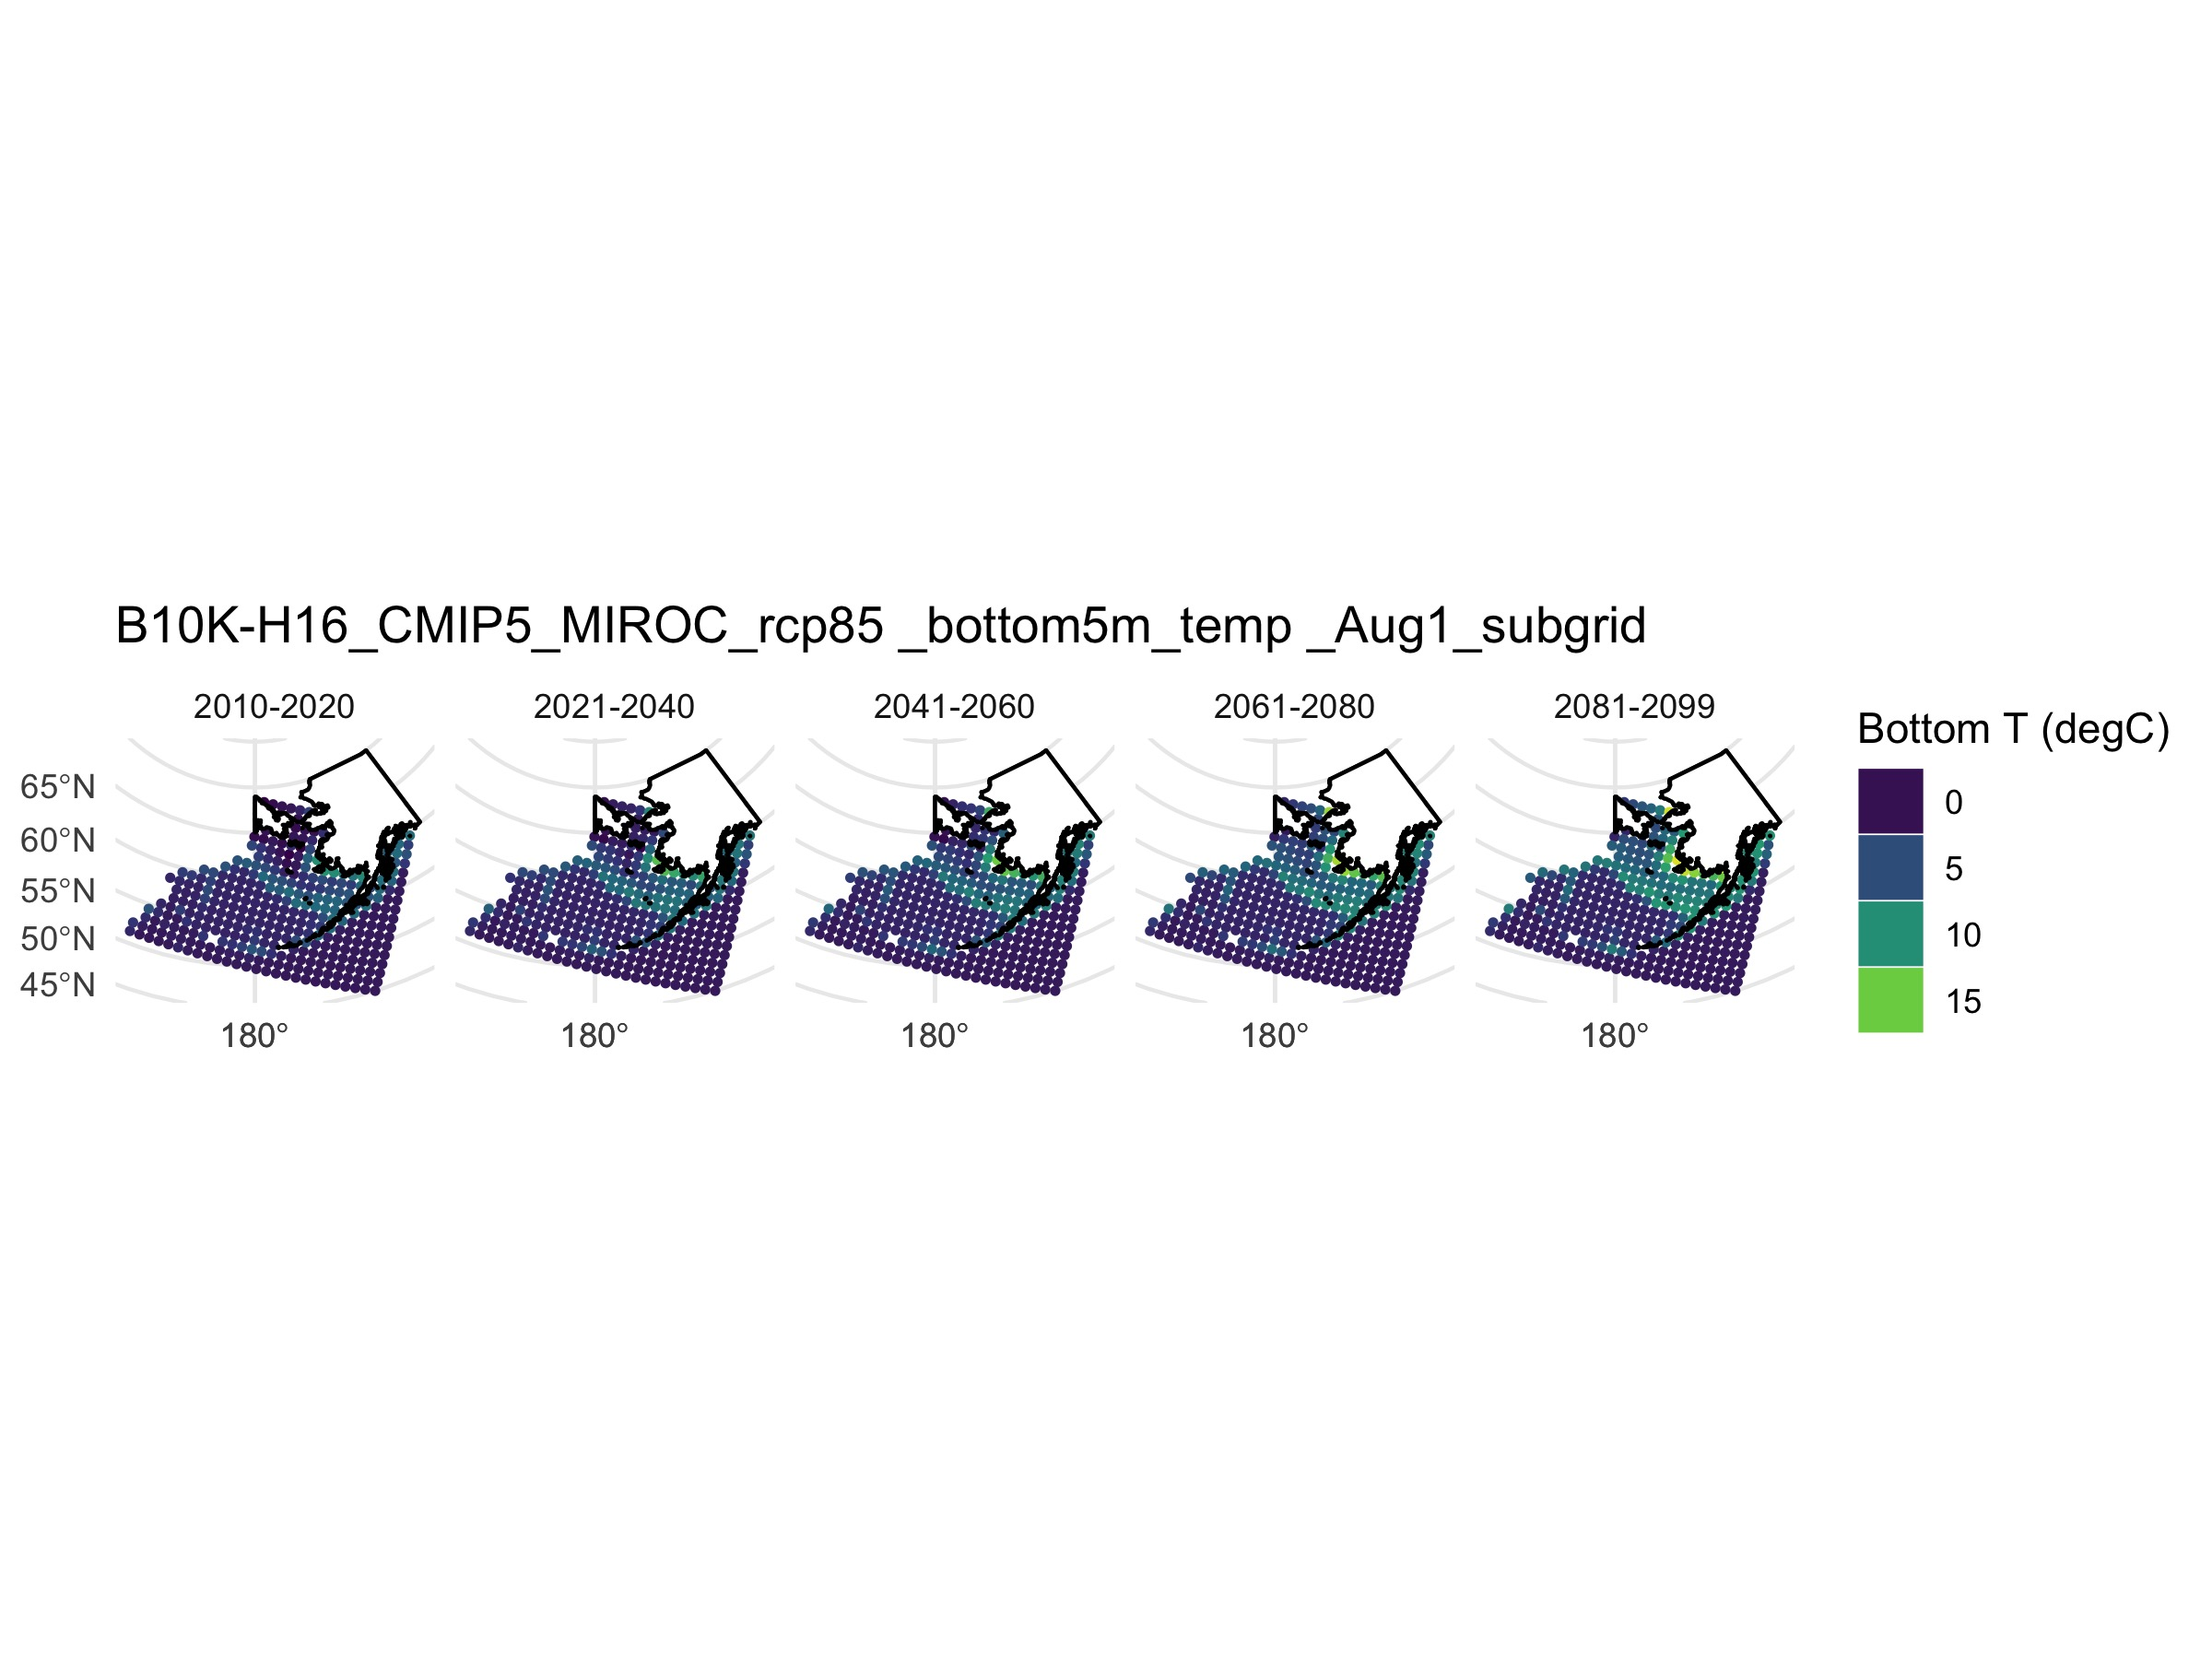
\includegraphics[width=0.65\textwidth,height=\textheight]{Figs/sub_grid_mn_BT_Aug1.jpg}
\#\#\# 6.2.2 Level 2 projections: Projections at M2 mooring

\hypertarget{funding-and-acknowledgments-needs-updating}{%
\section{7. Funding and acknowledgments (needs
updating):}\label{funding-and-acknowledgments-needs-updating}}

\hypertarget{acknowledgements-suggestion-projections}{%
\subsection{7.1 Acknowledgements suggestion:
projections}\label{acknowledgements-suggestion-projections}}

\hypertarget{please-include-a-statement-like-the-following-one-in-your-acknowledgements-section}{%
\subsubsection{PLEASE Include a statement like the following one in your
acknowledgements
section:}\label{please-include-a-statement-like-the-following-one-in-your-acknowledgements-section}}

\emph{This study is part of NOAA's Alaska Climate Integrated Modeling
project (ACLIM) and FATE project XXXX. We would like to that the entire
ACLIM team including \texttt{{[}add\ specific\ names{]}} for feedback
and discussions on the broader application of this work. Multiple NOAA
National Marine Fisheries programs provided support for ACLIM including
Fisheries and the Environment (FATE), Stock Assessment Analytical
Methods (SAAM) Science and Technology North Pacific Climate Regimes and
Ecosystem Productivity, the Integrated Ecosystem Assessment Program
(IEA), the NOAA Economics and Social Analysis Division, NOAA Research
Transition Acceleration Program (RTAP), the Alaska Fisheries Science
Center (ASFC), the Office of Oceanic and Atmospheric Research (OAR) and
the National Marine Fisheries Service (NMFS). The scientific views,
opinions, and conclusions expressed herein are solely those of the
authors and do not represent the views, opinions, or conclusions of NOAA
or the Department of Commerce.}

\hypertarget{for-some-of-the-integrated-papers-the-following-maybe-should-also-be-added}{%
\subsubsection{For some of the integrated papers the following maybe
should also be
added:}\label{for-some-of-the-integrated-papers-the-following-maybe-should-also-be-added}}

\emph{Additionally, the International Council for the Exploration of the
Sea (ICES) and the North Pacific Marine Science Organization (PICES)
provided support for Strategic Initiative for the Study of Climate
Impacts on Marine Ecosystems (SI-CCME) workshops, which facilitated
development of the ideas presented in this paper. The scientific views,
opinions, and conclusions expressed herein are solely those of the
authors and do not represent the views, opinions, or conclusions of
NOAA, the Department of Commerce, ICES, or PICES.}

\hypertarget{helpful-links-and-further-reading}{%
\section{8. Helpful links and further
reading:}\label{helpful-links-and-further-reading}}

\hypertarget{citations-for-gcms-and-carbon-scenarios}{%
\subsection{8.1 Citations for GCMs and carbon
scenarios:}\label{citations-for-gcms-and-carbon-scenarios}}

\hypertarget{cmip3-bsierp-global-climate-model-runs}{%
\subsubsection{CMIP3 (BSIERP global climate model
runs):}\label{cmip3-bsierp-global-climate-model-runs}}

Meehl, G. A., C. Covey, T. Delworth, M. Latif, B. McAvaney, J. F. B.
Mitchell, R. J. Stouffer, and K. E. Taylor, 2007: The WCRP CMIP3
multimodel dataset: A new era in climate change research. Bull. Amer.
Meteor. Soc., 88, 1383--1394.

\hypertarget{cmip5-aclim-global-climate-model-runs}{%
\subsubsection{CMIP5 (ACLIM global climate model
runs):}\label{cmip5-aclim-global-climate-model-runs}}

Taylor, K. E., R. J. Stouffer, and G. A. Meehl, 2012:Anoverview of CMIP5
and the experiment design. Bull. Amer. Meteor. Soc., 93, 485--498.

\hypertarget{cmip6-and-ssps-aclim2-global-climate-model-runs}{%
\subsubsection{CMIP6 and SSPs (ACLIM2 global climate model
runs):}\label{cmip6-and-ssps-aclim2-global-climate-model-runs}}

ONeill, B. C., C. Tebaldi, D. P. van Vuuren, V. Eyring, P.
Friedlingstein, G. Hurtt, R. Knutti, E. Kriegler, J.-F. Lamarque, J.
Lowe, G. A. Meehl, R. Moss, K. Riahi, and B. M. Sanderson. 2016. The
Scenario Model Intercomparison Project (ScenarioMIP) for CMIP6.
Geoscientific Model Development 9:3461--3482.

\hypertarget{weblinks-for-further-reading}{%
\subsection{8.2 Weblinks for further
reading:}\label{weblinks-for-further-reading}}

\begin{itemize}
\item
  Explore annual indices of downscaled projections for the EBS:
  \href{https://kholsman.shinyapps.io/aclim/}{\textbf{ACLIM indices}}
\item
  To view climate change projections from CMIP5 (eventually
  CMIP6):\href{https://www.esrl.noaa.gov/psd/ipcc/ocn/}{\textbf{ESRL
  climate change portal }}
\end{itemize}

\hypertarget{additional-information-on-hindcast-and-projection-models-needs-updating}{%
\subsection{8.3 Additional information on Hindcast and Projection Models
(needs
updating)}\label{additional-information-on-hindcast-and-projection-models-needs-updating}}

\hypertarget{core-cfsr-1976-2012}{%
\subsubsection{CORE-CFSR (1976-2012)}\label{core-cfsr-1976-2012}}

This is the hindcast for the Bering Sea and is a combination of the
reconstructed climatology from the
\href{http://portal.aoos.org/bering-sea.php\#module-metadata/5626a0b6-7d79-11e3-ac17-00219bfe5678/0756e6c2-a8e2-40af-aa3d-22051ed68067}{\textbf{CLIVAR}}
Co-ordinated Ocean-Ice Reference Experiments (CORE) Climate Model
(1969-2006) the
\href{http://portal.aoos.org/bering-sea.php\#module-metadata/f8cb79f6-7d59-11e3-a6ee-00219bfe5678/2deb2eca-f3f5-4eda-a132-112468711de7}{\textbf{NCEP}}
Climate Forecast System Reanalysis is a set of re-forecasts carried out
by NOAA's National Center for Environmental Prediction (NCEP). See
\href{http://cfs.ncep.noaa.gov/cfsr/}{\textbf{CFS-R}} for more info.

\hypertarget{cccma2006-2039-ar4-sres-a1b}{%
\subsubsection{\texorpdfstring{\href{http://www.cccma.ec.gc.ca/diagnostics/cgcm3/cgcm3.shtml}{CCCMA}(2006-2039;
AR4 SRES
A1B)}{CCCMA(2006-2039; AR4 SRES A1B)}}\label{cccma2006-2039-ar4-sres-a1b}}

Developed by the Canadian Centre for Climate Modelling and Analysis,
this is also known as the CGCM3/T47 model. This model showed the
greatest warming over time compared to other models tested by PMEL. See
more data the
\href{http://portal.aoos.org/bering-sea.php\#module-metadata/4f706756-7d57-11e3-bce5-00219bfe5678/ffa1bcc1-288d-4f8e-912e-500a618b241a}{\textbf{AOOS:CCCMA
portal}}.

\hypertarget{echog2006-2039-ar4-sres-a1b}{%
\subsubsection{\texorpdfstring{\href{http://www-pcmdi.llnl.gov/ipcc/model_documentation/ECHO-G.pdf}{ECHOG}(2006-2039;
AR4 SRES
A1B)}{ECHOG(2006-2039; AR4 SRES A1B)}}\label{echog2006-2039-ar4-sres-a1b}}

The ECHO-G model from the Max Planck Institute in Germany This model
showed the least warming over time compared to other models tested by
PMEL. See more data the AOOS:ECHO-G portal.

\hypertarget{gfdl-2006-2100-ar5-rcp-4.5-8.5-ssp126ssp585}{%
\subsubsection{\texorpdfstring{\href{http://www.gfdl.noaa.gov/earth-system-model}{GFDL}
(2006-2100; AR5 RCP 4.5, 8.5,
SSP126,SSP585)}{GFDL (2006-2100; AR5 RCP 4.5, 8.5, SSP126,SSP585)}}\label{gfdl-2006-2100-ar5-rcp-4.5-8.5-ssp126ssp585}}

The NOAA Geophysical Fluid Dynamics Laboratory
\href{http://www.gfdl.noaa.gov}{\textbf{GFDL}} has lead development of
the first Earth System Models (ESMs), which like physical climate
models, are based on an atmospheric circulation model coupled with an
oceanic circulation model, with representations of land, sea ice and
iceberg dynamics; ESMs additionally incorporate interactive
biogeochemistry, including the carbon cycle. The ESM2M model used in
this project is an evolution of the prototype EMS2.1 model, where
pressure-based vertical coordinates are used along the developmental
path of GFDL's Modular Ocean Model version 4.1 and where the land model
is more adavanced (LM3) than in the previous ESM2.1

\hypertarget{miroc2006-2039-ar4-sres-a1b-2006-2100-rcp4.5-rcp8.5-ssp585-ssp126}{%
\subsubsection{\texorpdfstring{\href{www.cger.nies.go.jp/publications/report/i073/I073.pdf}{MIROC}(2006-2039;
AR4 SRES A1B; 2006-2100 RCP4.5, RCP8.5, SSP585,
SSP126)}{MIROC(2006-2039; AR4 SRES A1B; 2006-2100 RCP4.5, RCP8.5, SSP585, SSP126)}}\label{miroc2006-2039-ar4-sres-a1b-2006-2100-rcp4.5-rcp8.5-ssp585-ssp126}}

The Model for Interdisciplinary Research on Climate (MIROC)-M model
developed by a consortium of agencies in Japan {[}{]}. Compared to other
models tested by PMEL, MIROC-M was intermediate in degree of warming
over the Bering Sea shelf for the first half of the 21st century. See
more data the AOOS:MIROC portal.

\end{document}
